%%==================================================
%% demo.tex for BIT Thesis
%% modified by yang yating
%% version: 1.0
%% last update: Sep. 1st, 2017
%%==================================================

% 默认单面打印 oneside 、硕士论文模板 master

\documentclass[oneside, master]{BIT-thesis-grd}

% 打印选项: 双面打印 oneside;单面打印 twoside
% 模板选项: 硕士论文 master; 博士论文 doctor

% 额外需要的库
\usepackage{fancyhdr}
\usepackage{graphicx}
\usepackage{caption}
\usepackage{multirow} 
\usepackage{amsmath}
\usepackage{amsfonts}
%\usepackage{subcaption}			不能与cls中的subfigure同时使用
%\usepackage[english]{babel}   		附录和参考文献的标题是英文



\begin{document}

%%%%%%%%%%%%%%%%%%%%%%%%%%%%%%
%% 封面
%%%%%%%%%%%%%%%%%%%%%%%%%%%%%%

% 中文封面内容(关注内容而不是形式)
\classification{V249}
\UDC{620}

\title{基于单目视觉的无人机同步定位与地图重建}
\vtitle{基于单目视觉的无人机同步定位与地图重建}

\author{孟超}
\institute{宇航学院}
\advisor{郭百巍副教授}
\chairman{徐勇副教授}
\degree{工学硕士}
\major{航空宇航科学与技术}
\school{北京理工大学}
\defenddate{2018年1月}
\studentnumber{2120150068}

% 英文封面内容(关注内容而不是表现形式)
\englishtitle{UAV Simultaneous Localization and Mapping\\Using Monocular Vision}
\englishauthor{Chao Meng}
\englishadvisor{Prof. Baiwei Guo}
\englishchairman{Prof. Yong Xu}
\englishschool{Beijing Insititute of Technology}
\englishinstitute{School of Aerospace Engineering}
\englishdegree{Master of Engineering}
\englishmajor{Aeronautical Science and Technology}
\englishdate{1,2018}

% 封面,这个命令实现了形式,具体见.cls
\maketitle

% 中文信息
\makeInfo

% 英文信息
\makeEnglishInfo

%打印竖排论文题目
\makeVerticalTitle

% 论文原创性声明和使用授权
\makeDeclareOriginal

%%%%%%%%%%%%%%%%%%%%%%%%%%%%%%
%% 前置部分前言
%%%%%%%%%%%%%%%%%%%%%%%%%%%%%%
\frontmatter

% 摘要
%%==================================================
%% abstract.tex for BIT Master Thesis
%% modified by yang yating
%% version: 0.1
%% last update: Dec 25th, 2016

%% modified by Meng Chao
%% version: 0.2
%% last update: May 29th, 2017
%%==================================================

\begin{abstract}
 
本文……。({\color{blue}{摘要是一篇具有独立性和完整性的短文,应概括而扼要地反映出本论文的主要内容。包括研究目的、研究方法、研究结果和结论等,特别要突出研究结果和结论。中文摘要力求语言精炼准确,硕士学位论文摘要建议500$\sim$800字,博士学位论文建议1000$\sim$1200字。摘要中不可出现参考文献、图、表、化学结构式、非公知公用的符号和术语。英文摘要与中文摘要的内容应一致。}})

\keywords{形状记忆;聚氨酯;织物;合成;应用 ({\color{blue}{一般选3~8个单词或专业术语,且中英文关键词必须对应。})}}

\end{abstract}

\begin{englishabstract}

   In this papers, we accomplish simultaneous localization and mapping using the monocular LSD-SLAM. This method is different with feature method, estimating the accurate and reconstructing the large scale environment map. Using the direct image alignment, the environment can be mapped in pose-graph of key frames semi-dense maps. The LSD-SLAM contains two advantage. A novel direct tracking method can definitely estimate the scale-drift. In addition, the probabilistic estimation can optimize the effect of noisy depth values on tracking. The experiment showed the LSD-SLAM is reliability, robustness and real-time.
   
\englishkeywords{direct image alignment; LSD-SLAM; probabilistic estimation; semi-dense maps}

\end{englishabstract}


% 加入目录
\tableofcontents

% 加入表格索引
%\listoftables

% 加入插图索引
%\listoffigures

%%%%%%%%%%%%%%%%%%%%%%%%%%%%%%
%% 正主体部分
%%%%%%%%%%%%%%%%%%%%%%%%%%%%%%


\mainmatter

% 各章正文内容
%%==================================================
%% chapter01.tex for BIT Master Thesis
%% modified by yang yating
%% version: 0.1
%% last update: Dec 25th, 2016

%% modified by Meng Chao
%% version: 0.2
%% last update: May 29th, 2017
%%==================================================
\chapter{绪论}
\label{chap:intro}

\section{论文研究目的与意义}


\section{无人机定位技术发展现状}


\section{视觉SLAM发展现状}



\section{论文主要内容和结构安排}




\begin{figure}
  \centering
  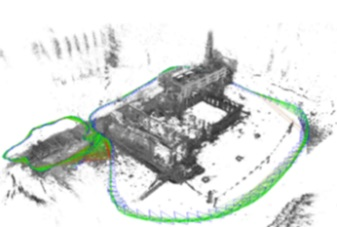
\includegraphics[height=0.5\textwidth]{figures/Fig1(1)}
  %\caption{The UAV equipped with an ASUS Xtion Pro Live RGB-D camera}
  %\label{Figure1.};
  
  \centering
  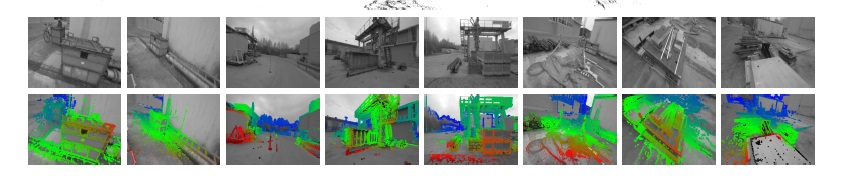
\includegraphics[width=0.75\textwidth]{figures/Fig1(2)}
  \caption{LSD-SLAM generates a consistent global map}
  %\label{referencename};
\end{figure}


%%==================================================
%% chapter02.tex for BIT Master Thesis
%% modified by yang yating
%% version: 0.1
%% last update: Dec 25th, 2016

%% modified by Meng Chao
%% version: 0.2
%% last update: May 29th, 2017
%%==================================================
\chapter{多旋翼无人机控制系统设计}
\label{chap:control design}
本章主要介绍多旋翼无人机数学模型和控制算法设计,研究多旋翼无人机的运动特性,便于之后分析和选择适合多旋翼无人机的视觉定位算法。

%2.1
\section{多旋翼无人机建模}
多旋翼无人机模型如图\ref{fig2.1}所示,分为四个部分:刚体运动学模型,刚体动力学模型,控制效率模型和动力单元模型。刚体运动学模型与无人机的质量和受力无关,以质点为模型研究无人机位置、速度、姿态、角速度等参量的变化。刚体动力学模型,研究物体所受力和力矩与运动状态变化的关系。多旋翼无人机与一般刚体动力学模型最大的不同在于螺旋桨拉力方向始终与机体坐标系$z_b$轴的负方向一致,以上两个模型又统称为刚体模型。控制效率模型研究不同机型对螺旋桨拉力和力矩的分配情况。动力单元模型则研究多旋翼无人机动力装置电机的数学模型。
\begin{figure}[h]
\centering
%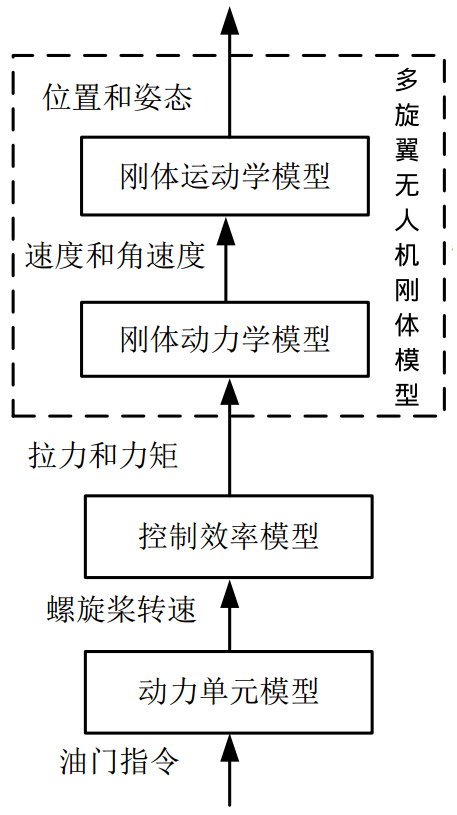
\includegraphics[scale=0.4]{figures/Fig2.1.png}
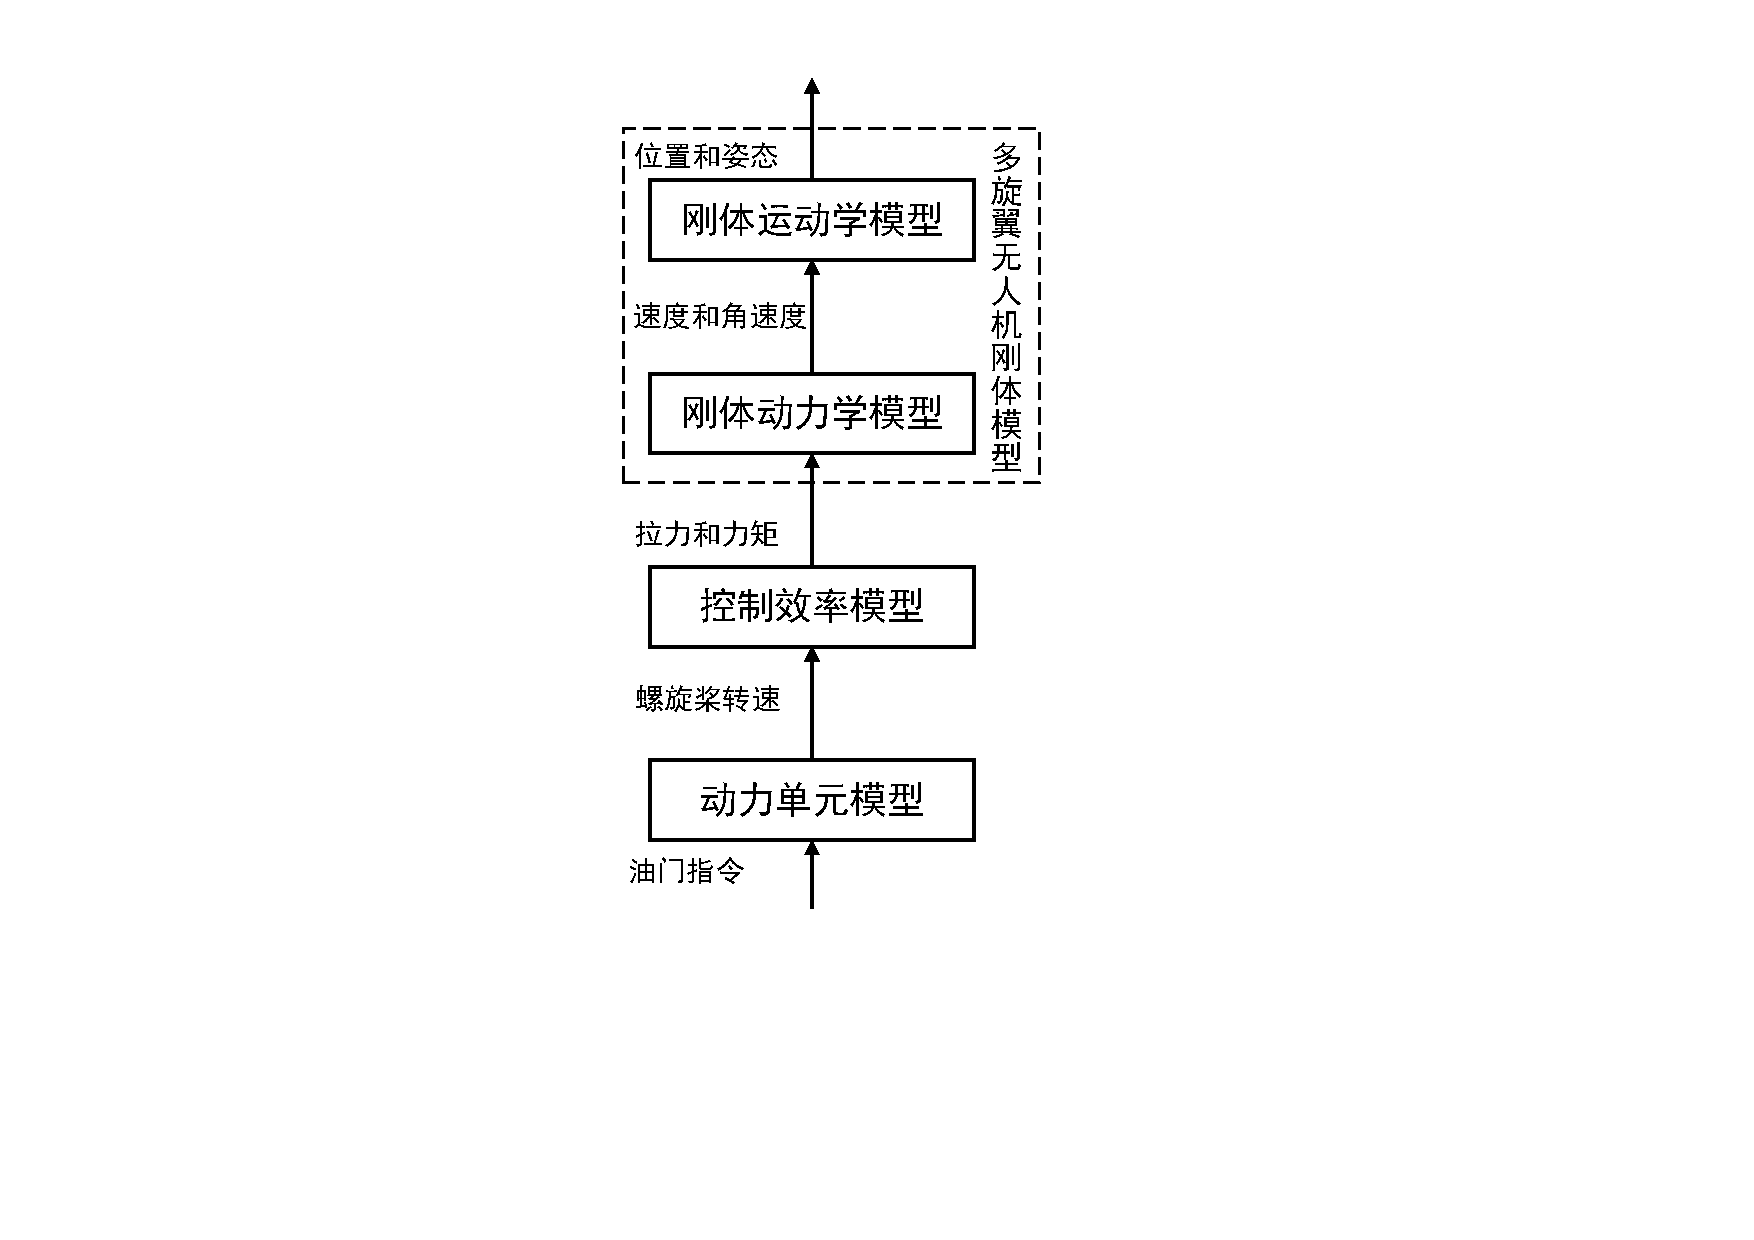
\includegraphics[scale=0.8,,angle=-90]{figures/Fig2-1.pdf}
\caption{多旋翼无人机模型}
\label{fig2.1}
\end{figure}

\subsection{坐标系定义与坐标变换}
多旋翼无人机的空间运动主要分为:质心运动和绕质心的运动,因而在描述任意时刻的空间运动时需要6个自由度:3个质心运动和3个角运动。在进行多旋翼无人机建模之前首先应该选择合适的坐标系,可以方便、准确的表示多旋翼无人机的空间状态和受力情况。本文在进行多旋翼无人机建模时主要用到连个坐标系:固联于无人机的机体坐标系和固定于无人机起飞点的地面坐标系,如图\ref{fig2.2}所示。\\
(1)机体坐标系$\boldsymbol{O} \boldsymbol{x}_b \boldsymbol{y}_b \boldsymbol{z}_b$

机体坐标系原点定义在多旋翼无人机质心上,$\boldsymbol{O} \boldsymbol{x}_b$平行于无人机前后旋翼,指向无人机前进的方向;$\boldsymbol{O} \boldsymbol{z}_b$位于无人机纵向平面,垂直向下;$\boldsymbol{O} \boldsymbol{y}_b$垂直于无人机纵向平面,方向根据右手定则确定。 \\ 
(2)地面坐标系$\boldsymbol{O} \boldsymbol{x}_e \boldsymbol{y}_e \boldsymbol{z}_e$

地面坐标系远点固定于无人机起飞位置,$\boldsymbol{O} \boldsymbol{x}_e$位于地平面内并指向无人机前进方向;$\boldsymbol{O} \boldsymbol{z}_e$垂直与地面并指向地心;$\boldsymbol{O} \boldsymbol{y}_e$位于地面平内,方向根据右手定则确定。

\begin{figure}[h]
\centering
%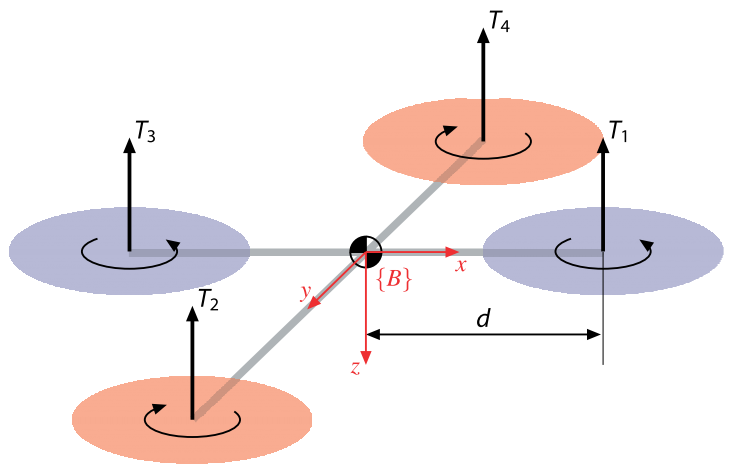
\includegraphics[scale=0.5]{figures/Fig2.2.png}
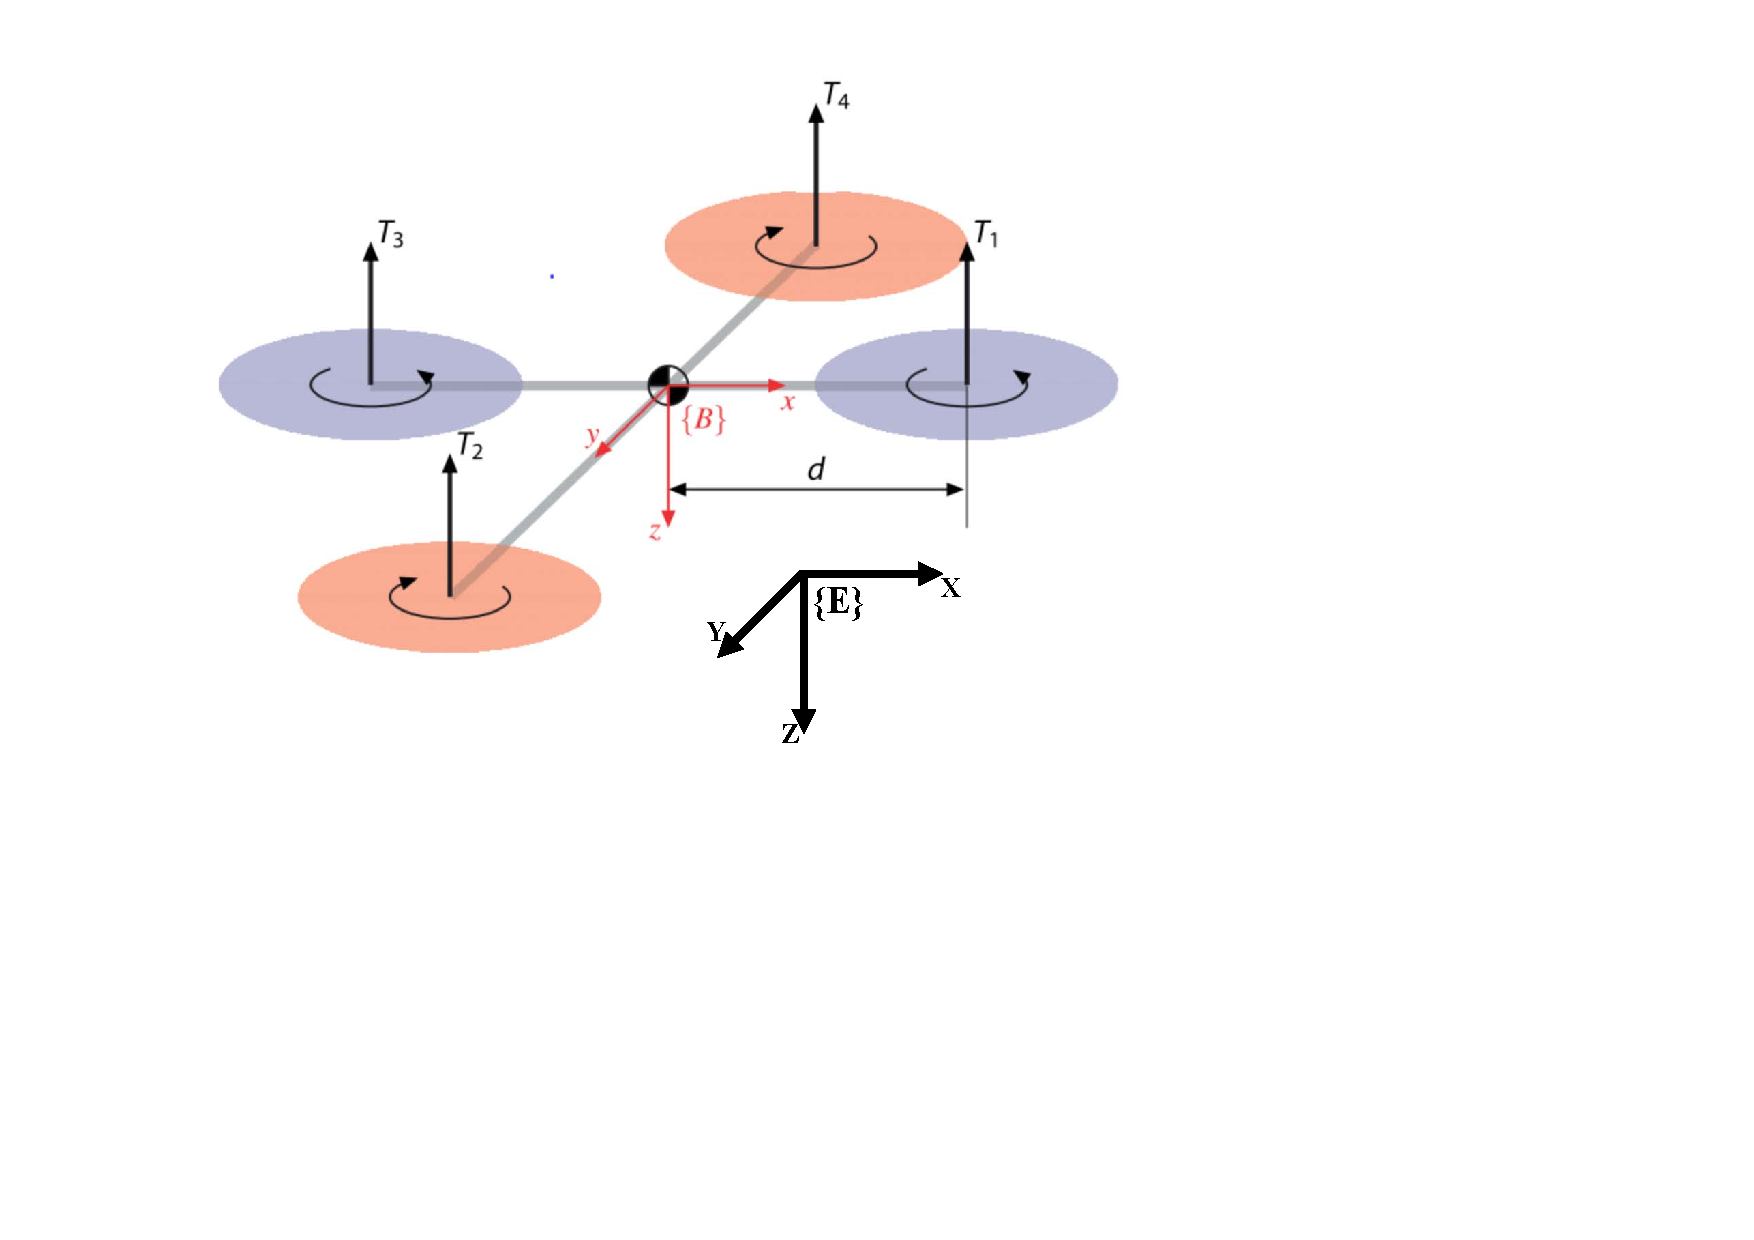
\includegraphics[scale=0.7,angle=-90]{figures/Fig2-2.pdf}
\caption{多旋翼无人机坐标系定义}
\label{fig2.2}
\end{figure}

为了便于描述无人机的空间运动状态,必须选择合适的坐标系,例如选择使用机体坐标系描述空间绕质心的运动,使用地面坐标系描述空间质心运动。当不同坐标系之间需要进行坐标转换,如将机体坐标系受到的螺旋桨拉力转换到地面坐标系分析质心运动。因而,坐标转换是无人机建模不可获取的一部分。一般机体坐标系与地面坐标系之间的转换关系可以由三个姿态角表示,偏航角$\psi$,俯仰角$\theta$和滚转角$\phi$。\\
1).俯仰角$\theta$:机体坐标系$\boldsymbol{O} \boldsymbol{x}_b$轴与地平面之间的夹角,沿$\boldsymbol{O} \boldsymbol{y}_b$轴顺时针旋转抬头为正。\\
2).滚转角$\phi$:机体坐标系$\boldsymbol{O} \boldsymbol{z}_b$与通过机体坐标系$\boldsymbol{O} \boldsymbol{x}_b$轴的铅垂面之间的夹角,沿$\boldsymbol{O} \boldsymbol{x}_b$轴顺时针旋转向右滚转为正。\\
3).偏航角$\psi$:机体坐标系$\boldsymbol{O} \boldsymbol{x}_b$轴在地平面的投影与地面坐标系$\boldsymbol{O} \boldsymbol{x}_e$的夹角,沿$\boldsymbol{O} \boldsymbol{z}_b$轴顺时针旋转右偏为正。

地面坐标系到机体坐标系的转换可以通过欧拉转动定理绕三轴连续转动得到,首先绕地面坐标系$\boldsymbol{O} \boldsymbol{z}_e$转动偏航角$\psi$,得到过度坐标系$\boldsymbol{O} \boldsymbol{x}^{'} \boldsymbol{y}^{'} \boldsymbol{z}^{'}$;之后再由过度坐标系绕$\boldsymbol{O} \boldsymbol{y}^{'}$旋转俯仰角$\theta$,得到过度坐标系$\boldsymbol{O} \boldsymbol{x}^{''} \boldsymbol{y}^{''} \boldsymbol{z}^{''}$;最后由过度坐标系$\boldsymbol{O} \boldsymbol{x}^{''} \boldsymbol{y}^{''} \boldsymbol{z}^{''}$绕$\boldsymbol{O} \boldsymbol{x}^{''}$旋转滚转角$\phi$。则从地面坐标系到机体坐标系的旋转矩阵$\boldsymbol{R}_{BE}$为
\begin{equation}
\label{equ2.1}
\begin{aligned}
\boldsymbol{R}_{BE} 
&= \boldsymbol{R}(\boldsymbol{\phi}) \boldsymbol{R}(\boldsymbol{\theta}) \boldsymbol{R}(\boldsymbol{\psi}) \\ 
&= 
\begin{bmatrix}
\cos\theta \cos\psi & \cos\theta \sin\psi & -\sin\theta \cr
\sin\theta \cos\psi \sin\phi - \sin\psi \cos\phi & \sin\theta \sin\psi \sin\phi + \cos\psi \cos\phi & \cos\theta \sin\phi \cr
\sin\theta \cos\psi \cos\phi + \sin\psi \sin\phi & \sin\theta \sin\psi \cos\phi - \cos\psi \sin\phi & \cos\theta \cos\phi \cr
\end{bmatrix}
\end{aligned}
\end{equation}

\subsection{多旋翼无人机刚体模型}
在进行多旋翼无人机刚体建模前,首先对无人机做出如下假设
\begin{enumerate}  [itemindent=1em,label={(\arabic*)}]
\item 假设多旋翼无人机是刚体。
\item 假设多旋翼无人机的质量和转动惯量保持不变。
\item 假设多旋翼无人机的几何中心和重心重合。
\item 假设多旋翼无人机只受重力和螺旋桨的拉力。
\item 假设奇数编号的螺旋桨逆时针转动,偶数编号螺旋桨顺时针转动
\end{enumerate}
首先进行刚体运动学建模,刚体运动学模型描述了多旋翼无人机运动状态的变化。\\
(1) 质心运动学模型

研究地面坐标系下无人机的位置$\boldsymbol{P}_e = [X,Y,Z]^T$的变化,分解到三轴坐标上有。
\begin{equation}
\label{equ2.2}
\begin{aligned}
\dot{\boldsymbol{P}}_e &= \boldsymbol{V}_e \\
\begin{bmatrix}
\dot{X} \cr \dot{Y} \cr \dot{Z} \cr
\end{bmatrix}
&=
\begin{bmatrix}
V_x \cr V_y \cr V_z \cr
\end{bmatrix}
\end{aligned}
\end{equation}
(2) 质心转动模型

研究姿态角速率$\dot{\boldsymbol{\Theta}}=[\dot{\theta},\dot{\psi},\dot{\phi}]^T$与机体坐标系下的转动角速率$\boldsymbol{\omega}_b=[\omega_x , \omega_y , \omega_z]^T$的关系。根据地面坐标系与机体坐标系之间的变换关系有。
\begin{equation}
\label{equ2.3}
\begin{aligned}
\boldsymbol{\omega}_b & = \boldsymbol{R}_{EB} \dot{\boldsymbol{\psi}}+\boldsymbol{R}(\boldsymbol{\phi}) \dot{\boldsymbol{\theta}}+ \dot{\boldsymbol{\phi}} 
\\
\begin{bmatrix}
\omega_x \cr \omega_y \cr \omega_z \cr
\end{bmatrix}
& =
\begin{bmatrix}
0 & -\sin \theta & 1 \cr
\cos \phi & \cos \theta \sin \phi & 0 \cr
-\sin \phi & \cos \theta \cos \phi & 0 \cr
\end{bmatrix}
\begin{bmatrix}
\dot{\theta} \cr \dot{\psi}  \cr  \dot{\phi} \cr
\end{bmatrix}
\end{aligned}
\end{equation}
(3)质心动力学模型

质心动力学模型研究无人机受力与质心运动的关系。设机体坐标系下所有螺旋桨产生的总拉力$\boldsymbol{T}_b=[0,0,T]^{T}$,无人机受到的重力在世界坐标系下表示为$\boldsymbol{G}_e=[0,0,mg]^T$,则无人机的质心运动方程可以表示为
\begin{equation}
\label{equ2.4}
\begin{aligned}
m\boldsymbol{V}_e &= \boldsymbol{G}_e -  \boldsymbol{R}_{EB} \boldsymbol{T}_b
\end{aligned}
\end{equation}
(4)绕质心转动动力学模型

绕质心转动的动力学模型研究无人机所受力矩与其空间转动的关系。设无人机在机体坐标系下的转动惯量为
\begin{equation}
\label{equ2.5}
\boldsymbol{I}_b = 
\begin{bmatrix}
I_x & 0 & 0 \cr
0 & I_y & 0 \cr
0 & 0 & I_z \cr
\end{bmatrix}
\end{equation}
假设无人机受到的总力矩在世界坐标系下为$\boldsymbol{M}_e=[M_x,M_y,M_z]^T$,根据矢量绝对导数与相对导数关系,由角动量定理得
\begin{equation}
\label{equ2.6}
\begin{aligned}
\boldsymbol{M}_e &= {d\boldsymbol{H}_e \over dt} = {d\boldsymbol{H}_b \over dt} +  \boldsymbol{\omega}_b \times \boldsymbol{H}_b 
\\
\boldsymbol{M}_e &= \boldsymbol{I}_b \dot{\boldsymbol{\omega}}_b +\boldsymbol{\omega}_b \times \boldsymbol{I}_b \boldsymbol{\omega}_b 
\end{aligned}
\end{equation}
以上公式\eqref{equ2.2},\eqref{equ2.3},\eqref{equ2.4},\eqref{equ2.6}组成了多旋翼无人机的非线性刚体模型。

\subsection{多旋翼无人机控制效率模型}
多旋翼无人机控制效率模型研究无人机机型布局与螺旋桨的拉力和力矩分配的关系。以十字型四旋翼无人机为例,已知第$i$个螺旋桨的拉力为$\boldsymbol{F}_i$与电机转速$\omega_i$关系为$\boldsymbol{F}_i = c_T \omega_i^2$,总拉力为
\begin{equation}
\label{equ2.7}
\boldsymbol{T}_b = \sum\limits_{i=1}^4 \boldsymbol{F}_i =  \sum\limits_{i=1}^4 c_T \omega_i^2
\end{equation}
四旋翼无人机机臂长$d$,螺旋桨对机体坐标系三轴产生的力矩为,
\begin{equation}
\label{equ2.8}
\begin{aligned}
M_x &= d c_T \left( \omega_4^2 - \omega_2^2\right)
\\
M_y &= d c_T \left( \omega_1^2 - \omega_3^2\right)
\\
M_z &= d c_M \left( \omega_1^2 - \omega_2^2 + \omega_3^2 - \omega_4^2\right)
\end{aligned}
\end{equation}
公式\eqref{equ2.7},\eqref{equ2.8}中$c_T $表示与螺旋桨类型相关的常量,$c_M$表示螺旋桨反扭力常数,将以上两公式进行整理可以得到无人机动力分配模型
\begin{equation}
\label{equ2.9}
\begin{bmatrix}
T \cr M_x \cr M_y \cr M_z \cr 
\end{bmatrix}
=
\begin{bmatrix}
c_T & c_T & c_T & c_T  \cr
0 & -d c_T & 0 & d c_T \cr
d c_T & 0 & -d c_T & 0 \cr
c_M & c_M & c_M & c_M  \cr
\end{bmatrix}
\begin{bmatrix}
\omega_1^2 \cr \omega_2^2 \cr \omega_3^2 \cr \omega_4^2 \cr
\end{bmatrix}
\end{equation}


\subsection{多旋翼无人机动力单元模型}
多旋翼无人机一般选用直流无刷电机,无刷电机微分方程为
\begin{equation}
\label{equ2.10}
\begin{aligned}
u &= iR + L {di \over dt} + k_e \omega
\\
J_m {d\omega \over dt} &= M_m - M_{load}
\end{aligned}
\end{equation}
其中$u$表示电机电压,$i$为电机电流,$\omega$表示电机旋转角速度,$R$表示电机等效电阻,$L$表示电机线圈电感,$k_e$表示电机反电动势系数,$J_m$表示电机线圈的轴向转动惯量,$M_m=k_m i$表示电机输出力矩,$M_{load}$表示电机负载力矩。由于电机线圈电感较小,省略后可以化简得到多旋翼无人机动力单元模型
\begin{equation}
\label{equ2.11}
\begin{aligned}
i &= {(u-k_e \omega) \over R }
\\
J_m {d \omega \over dt} &= k_m{u \over R } - {k_e k_m \omega \over R} - M_{load}
\end{aligned}
\end{equation}

%2.2
\section{多旋翼无人机控制算法研究}
为了更好的控制飞行器运动,采用串级PID进行控制策略,分为两个控制器位置控制器和姿态控制器。位置控制器为外环,负责控制多旋翼无人机的位置;姿态控制器为内环,负责控制多旋翼无人机的姿态角。由内外环控制实现多旋翼飞行器的升降、悬停和侧飞等飞行模态,控制系统结构狂徒如图\ref{fig2.3}所示。
\begin{figure}[h]
\centering
%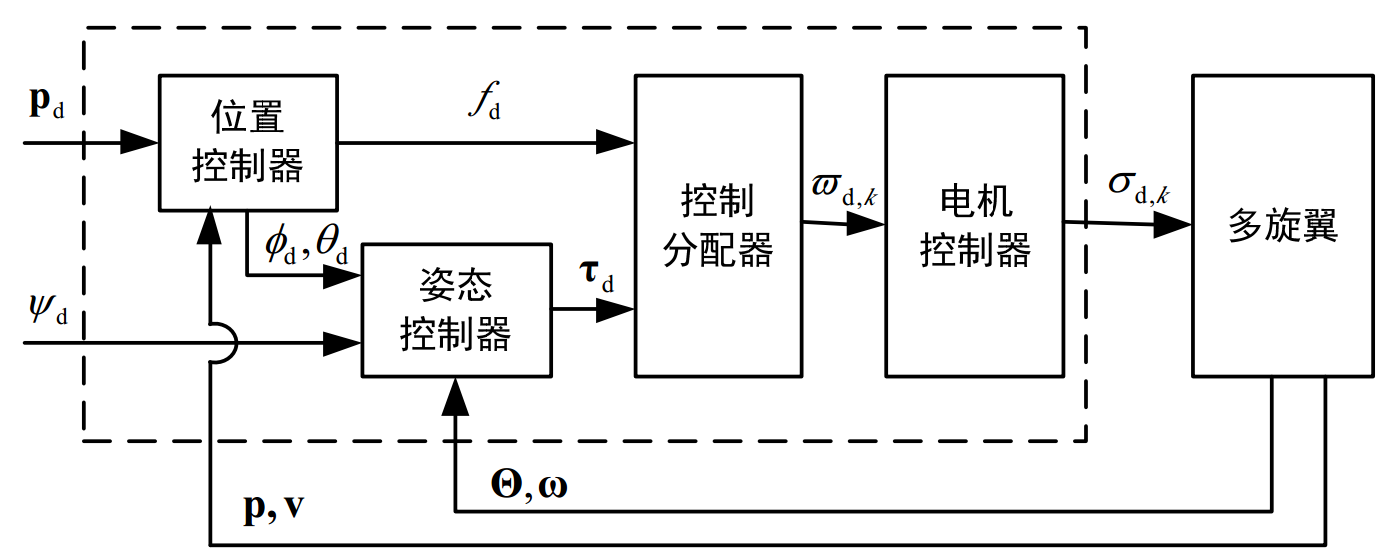
\includegraphics[scale=0.3]{figures/Fig2.3.png}
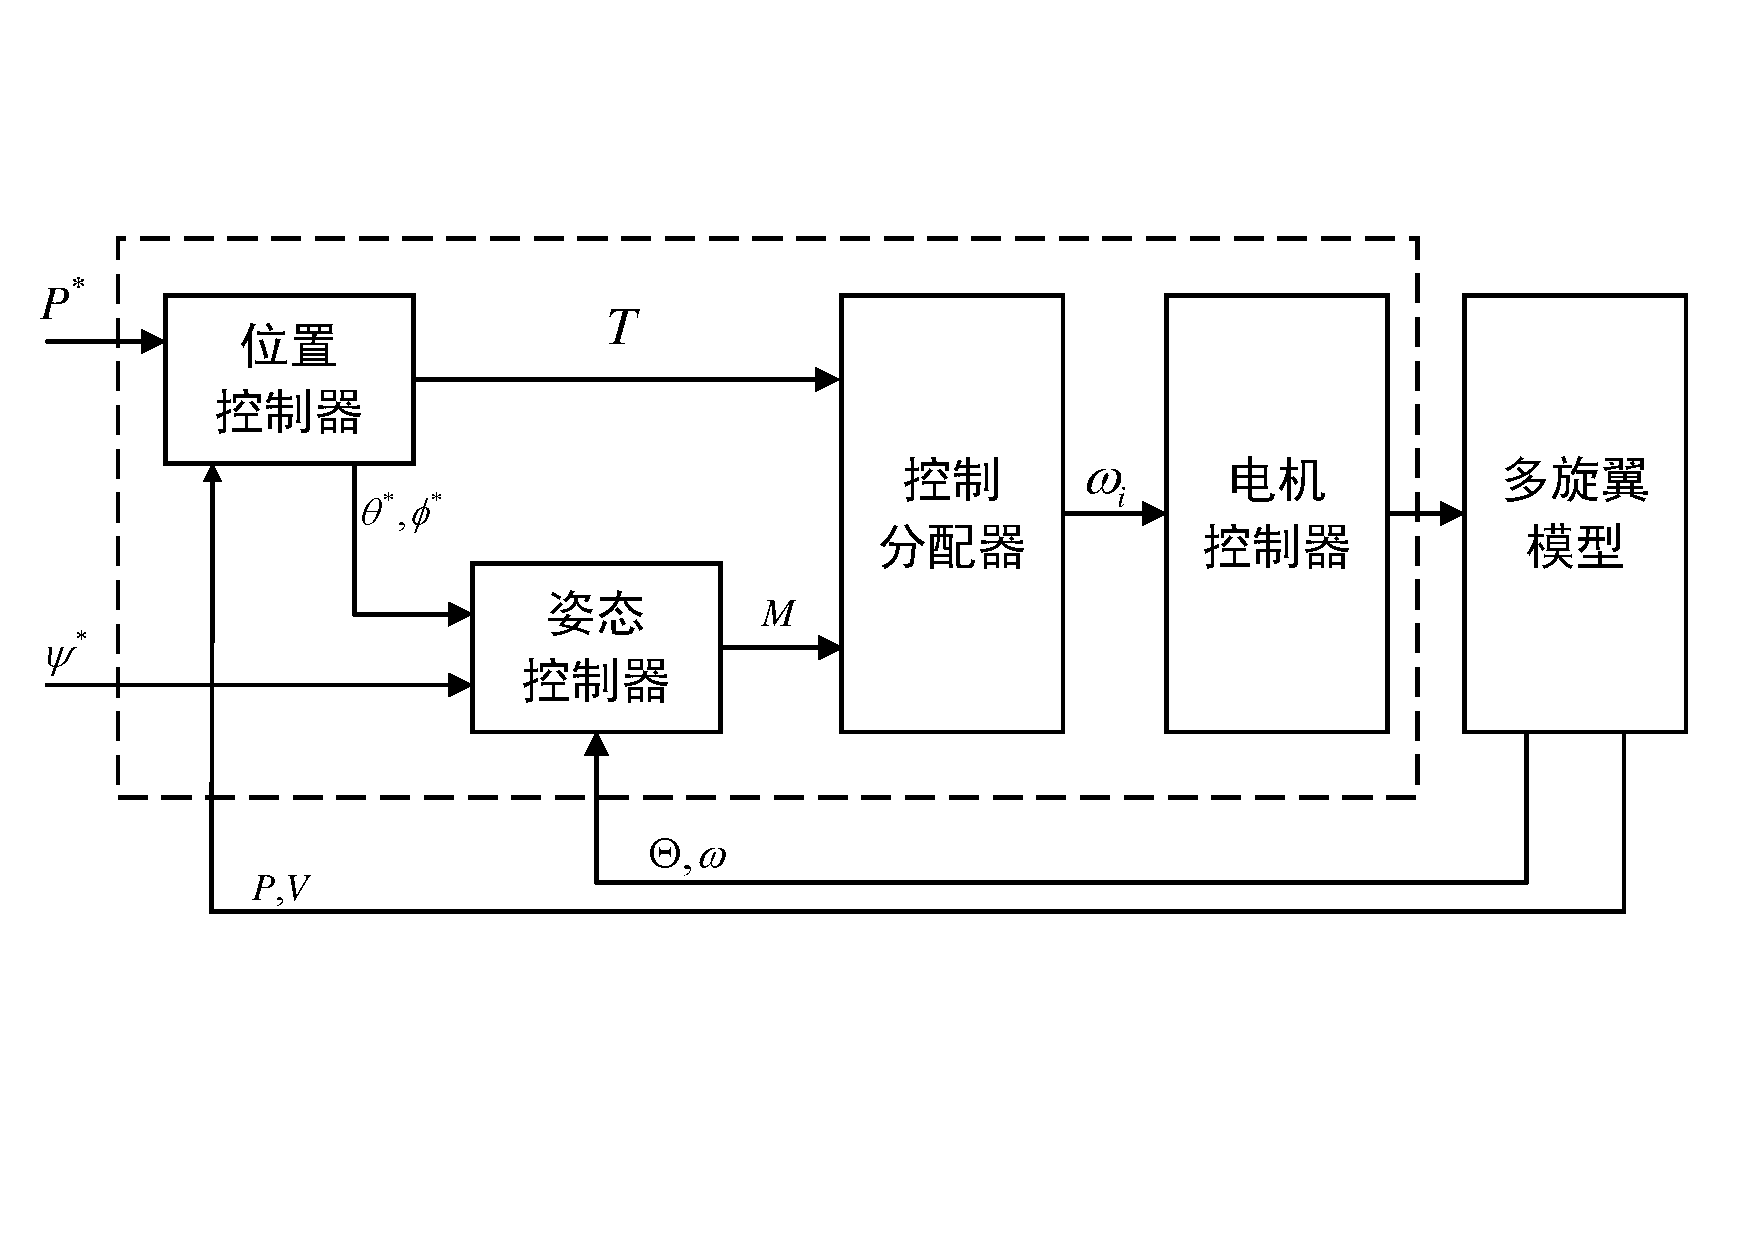
\includegraphics[scale=0.5,angle=-90]{figures/Fig2-3.pdf}
\caption{多旋翼无人机闭环控制框图}
\label{fig2.3}
\end{figure}

\subsection{姿态控制器}
多旋翼无人机的姿态角直接影响无人机的飞行状态,对于内环姿态控制器,根据方程\eqref{equ2.5}可知多旋翼飞行器绕质心转动的动力学模型为二阶系统,因而在姿态控制回路引入比例-微分控制器进行调节,并将控制通道解耦为俯仰/滚转通道和偏航通道。对于俯仰/滚转通道,多旋翼无人机的俯仰、滚转运动对称,因而以俯仰通道为例介绍,设计比例-微分控制器
\begin{equation}
\label{equ2.12}
\begin{aligned}
M_x &= K_{p\theta} \left( \theta^* - \theta \right) + K_{d\theta} \left( \dot{\theta}^* -  \dot{\theta} \right)
\end{aligned}
\end{equation}
其中$\theta^*$、$\dot{\theta}$表示反馈的姿态角和姿态角速率,$\theta^*$表示期望俯仰角,由位置控制器给出。$ \dot{\theta}^*$通常较小可以忽略。

对于偏航通道,同样采用比例-微分控制器
\begin{equation}
\label{equ2.13}
M_z = K_{p\psi} \left( \psi^* - \psi \right) + K_{d\psi} \left( \dot{\psi}^* -  \dot{\psi} \right)
\end{equation}
其中$\psi$、$\dot{\psi}$表示反馈的姿态角和姿态角速率。不同于俯仰/滚转通道,$\psi^*$表示的期望俯仰角不由位置控制器给出,而是根据规划的轨迹或外部遥控装置直接给出。$ \dot{\psi}^*$通常较小可以忽略。

\subsection{位置控制器}
对多旋翼无人机刚体运动学模型\eqref{equ2.3},\eqref{equ2.4}进行线性化近似可知,多旋翼无人机的水平运动影响俯仰/滚转姿态角变化,高度运动影响无人机推力变化。对于水平运动,$x$,$y$方向的运动是等价的,以x方向运动为例,设计比例控制器约束无人机的期望速度
\begin{equation}
\label{equ2.14}
v_x^* =  K_{px} \left( p_x^* - p_x \right)
\end{equation}
其中$p_x $表示反馈的$x$方向位置,$p_x^*$表示$x$方向的期望位置,$v_x^*$表示$x$方向的期望速度。根据\eqref{equ2.3}的现行近似模型可知,为了使机体产生沿$x$方向的运动,需要产生俯仰角,有
\begin{equation}
\label{equ2.15}
f_x = T \sin\theta \simeq T \theta
\end{equation}
根据方程\eqref{equ2.15}设计比例控制器
\begin{equation}
f_x = K_{vx} \left(  v_x^* - v_x \right)
\end{equation}
联立方程\eqref{equ2.14},\eqref{equ2.15}可以得到期望的俯仰姿态角$\theta^*$
\begin{equation}
\label{equ2.16}
\theta^* = K_{vx} \left( K_{px} \left( p_x^* - p_x \right) - v_x \right)
\end{equation}

对于高度控制器,设计比例-微分控制器调节多旋翼无人机的推力
\begin{equation}
\label{equ2.17}
T = K_{pz} \left( z^* -z  \right) + K_{dz} \left( \dot{z}^* - \dot{z}  \right) + G_0
\end{equation}
其中,$z^*$表示目标高度,$z$,$\dot{z}$表示无人机反馈的高度位置和速度。$G_0$是前馈控制量,抵消重力的影响,避免高度控制中的定常干扰。

%2.3
\section{ 数学仿真验证}



\section{本章小结}



\iffalse
%2.4
%\section{Weighted Gauss-Newton Optimization on Lie-Manifolds}
Two images are aligned by Gauss-Newton minimization of the photometric error
\begin{equation}
E(\xi)=\sum( I_{ref}(p_{i} - I( \omega( p_{i},D_{ref}(p_{i}),\xi ) ))^{2}
\end{equation}
which gives the maximum-likelihood estimator for ${\mathbf{\xi }}$ assuming Gaussian residuals. We use a left-compositional formulation. Starting with an initial estimate ${{\mathbf{\xi }}^{{\mathbf{(0)}}}}$, in each iteration a left-multiplied increment $\delta {{\mathbf{\xi }}^{{\mathbf{(n)}}}}$ is computed by solving for the minimum of Gauss-Newton second-order approximation of E.
\begin{equation}
\delta\xi^{n}=-(J^{T}J)^{-1}J^{T}r(\xi^{n}) \ with \  \left. J=\frac{\partial r(\varepsilon\circ\xi^{n})}{\partial \varepsilon} \right|_{\varepsilon=0}
\end{equation}

where ${\mathbf{J}}$ is the derivative of the stacked residual vector ${ r=(r_{1},...,r_{n})^{T} }$ with respect to a left-multiplied increment, and ${{\mathbf{J}}^{\mathbf{T}}}{\mathbf{J}}$ the Gauss-Newton approximation of the Hessian of $E$. The new estimate is then obtained by multiplication with the computed update

\begin{equation}
\xi ^{(n + 1)} = \delta \xi ^{(n)} \circ \xi ^{(n)}
\end{equation}

In order to be robust to outliers arising from occlusions or reflections, different weighting-schemes have been proposed by [7].

\begin{equation}
E(\xi)=\sum\limits_i \omega_{i}(\xi)r_{i}(\xi)
\end{equation}
and the update is computed as

\begin{equation}
\delta {\xi ^{(n)}} =  - (J^{T}WJ)^{ - 1}J^{T}W_{r}({\xi ^{(n)}})
\end{equation}

Assuming the residuals to be independent, the last iteration ${({J^T}WJ)^{ - 1}}$ is an estimate for the covariance   of a left-multiplied error onto the final result. The default type-implementation in g2o assumes right-multiplication [8].

\begin{equation}
\xi ^{(n)} = \varepsilon  \circ \xi _{true} \ with \ \varepsilon \sim N(0,\sum \varepsilon  )
\end{equation}
\fi




%%==================================================
%% chapter03.tex for BIT Master Thesis
%% modified by yang yating
%% version: 0.1
%% last update: Dec 25th, 2016

%% modified by Meng Chao
%% version: 0.2
%% last update: May 29th, 2017
%%==================================================
\chapter{单目SLAM算法研究}
\label{chap:ALGORITHM}

%3.1
%\section{引言}
同步定位与地图重建算法利用多视图几何原理\upcite{[]},根据获取的图像信息估计摄像头在陌生环境中的位姿,构建环境地图。如果获取图像信息时,仅使用一个摄像头,则称为单目SLAM。本章主要介绍经典视觉SLAM算法框架;研究基于该框架的两种主流单目SLAM算法,在相同数据集上对比分析两种算法的优缺点,结合无人机运动特性选择合适的SLAM算法。

%3.1
\section{经典视觉SLAM算法框架}
SLAM算法实际是状态估计问题,将传感器数据抽象为适于估计的数学模型,通过观测模型与运动模型估计系统状态。经典视觉SLAM算法框架一般包括3个部分:视觉里程计,后端优化和闭环检测。视觉里程计估计帧间运动和局部地图,把传感器数据抽象为适于估计的数学模型;后端优化则接收视觉里程计估计的不同时刻位姿和回环检测信息,根据观测模型和运动模型建立约束关系,估计优化相机位姿与地图点位置,得到全局一致的轨迹与地图;回环检测判断相机是否曾经到达过当前位置,如果检测到回环反馈则给后端进行优化处理。算法框架如图\ref{fig3.1}所示,经典的视觉SLAM算法框架是过去十几年研究者们总结的成果,框架本身和所包含的算法已经较为成熟。本文研究内容主要是在该框架的基础上,针对单目SLAM算法存在的问题进行改进和完善。

\begin{figure}[h]
\centering
%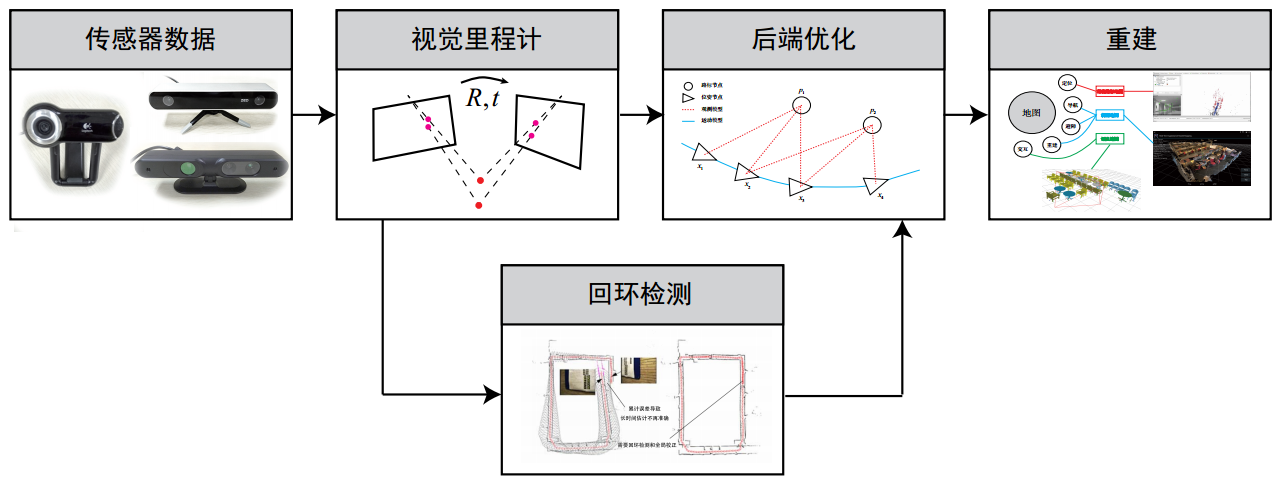
\includegraphics[scale=0.3]{figures/Fig3.1.png}
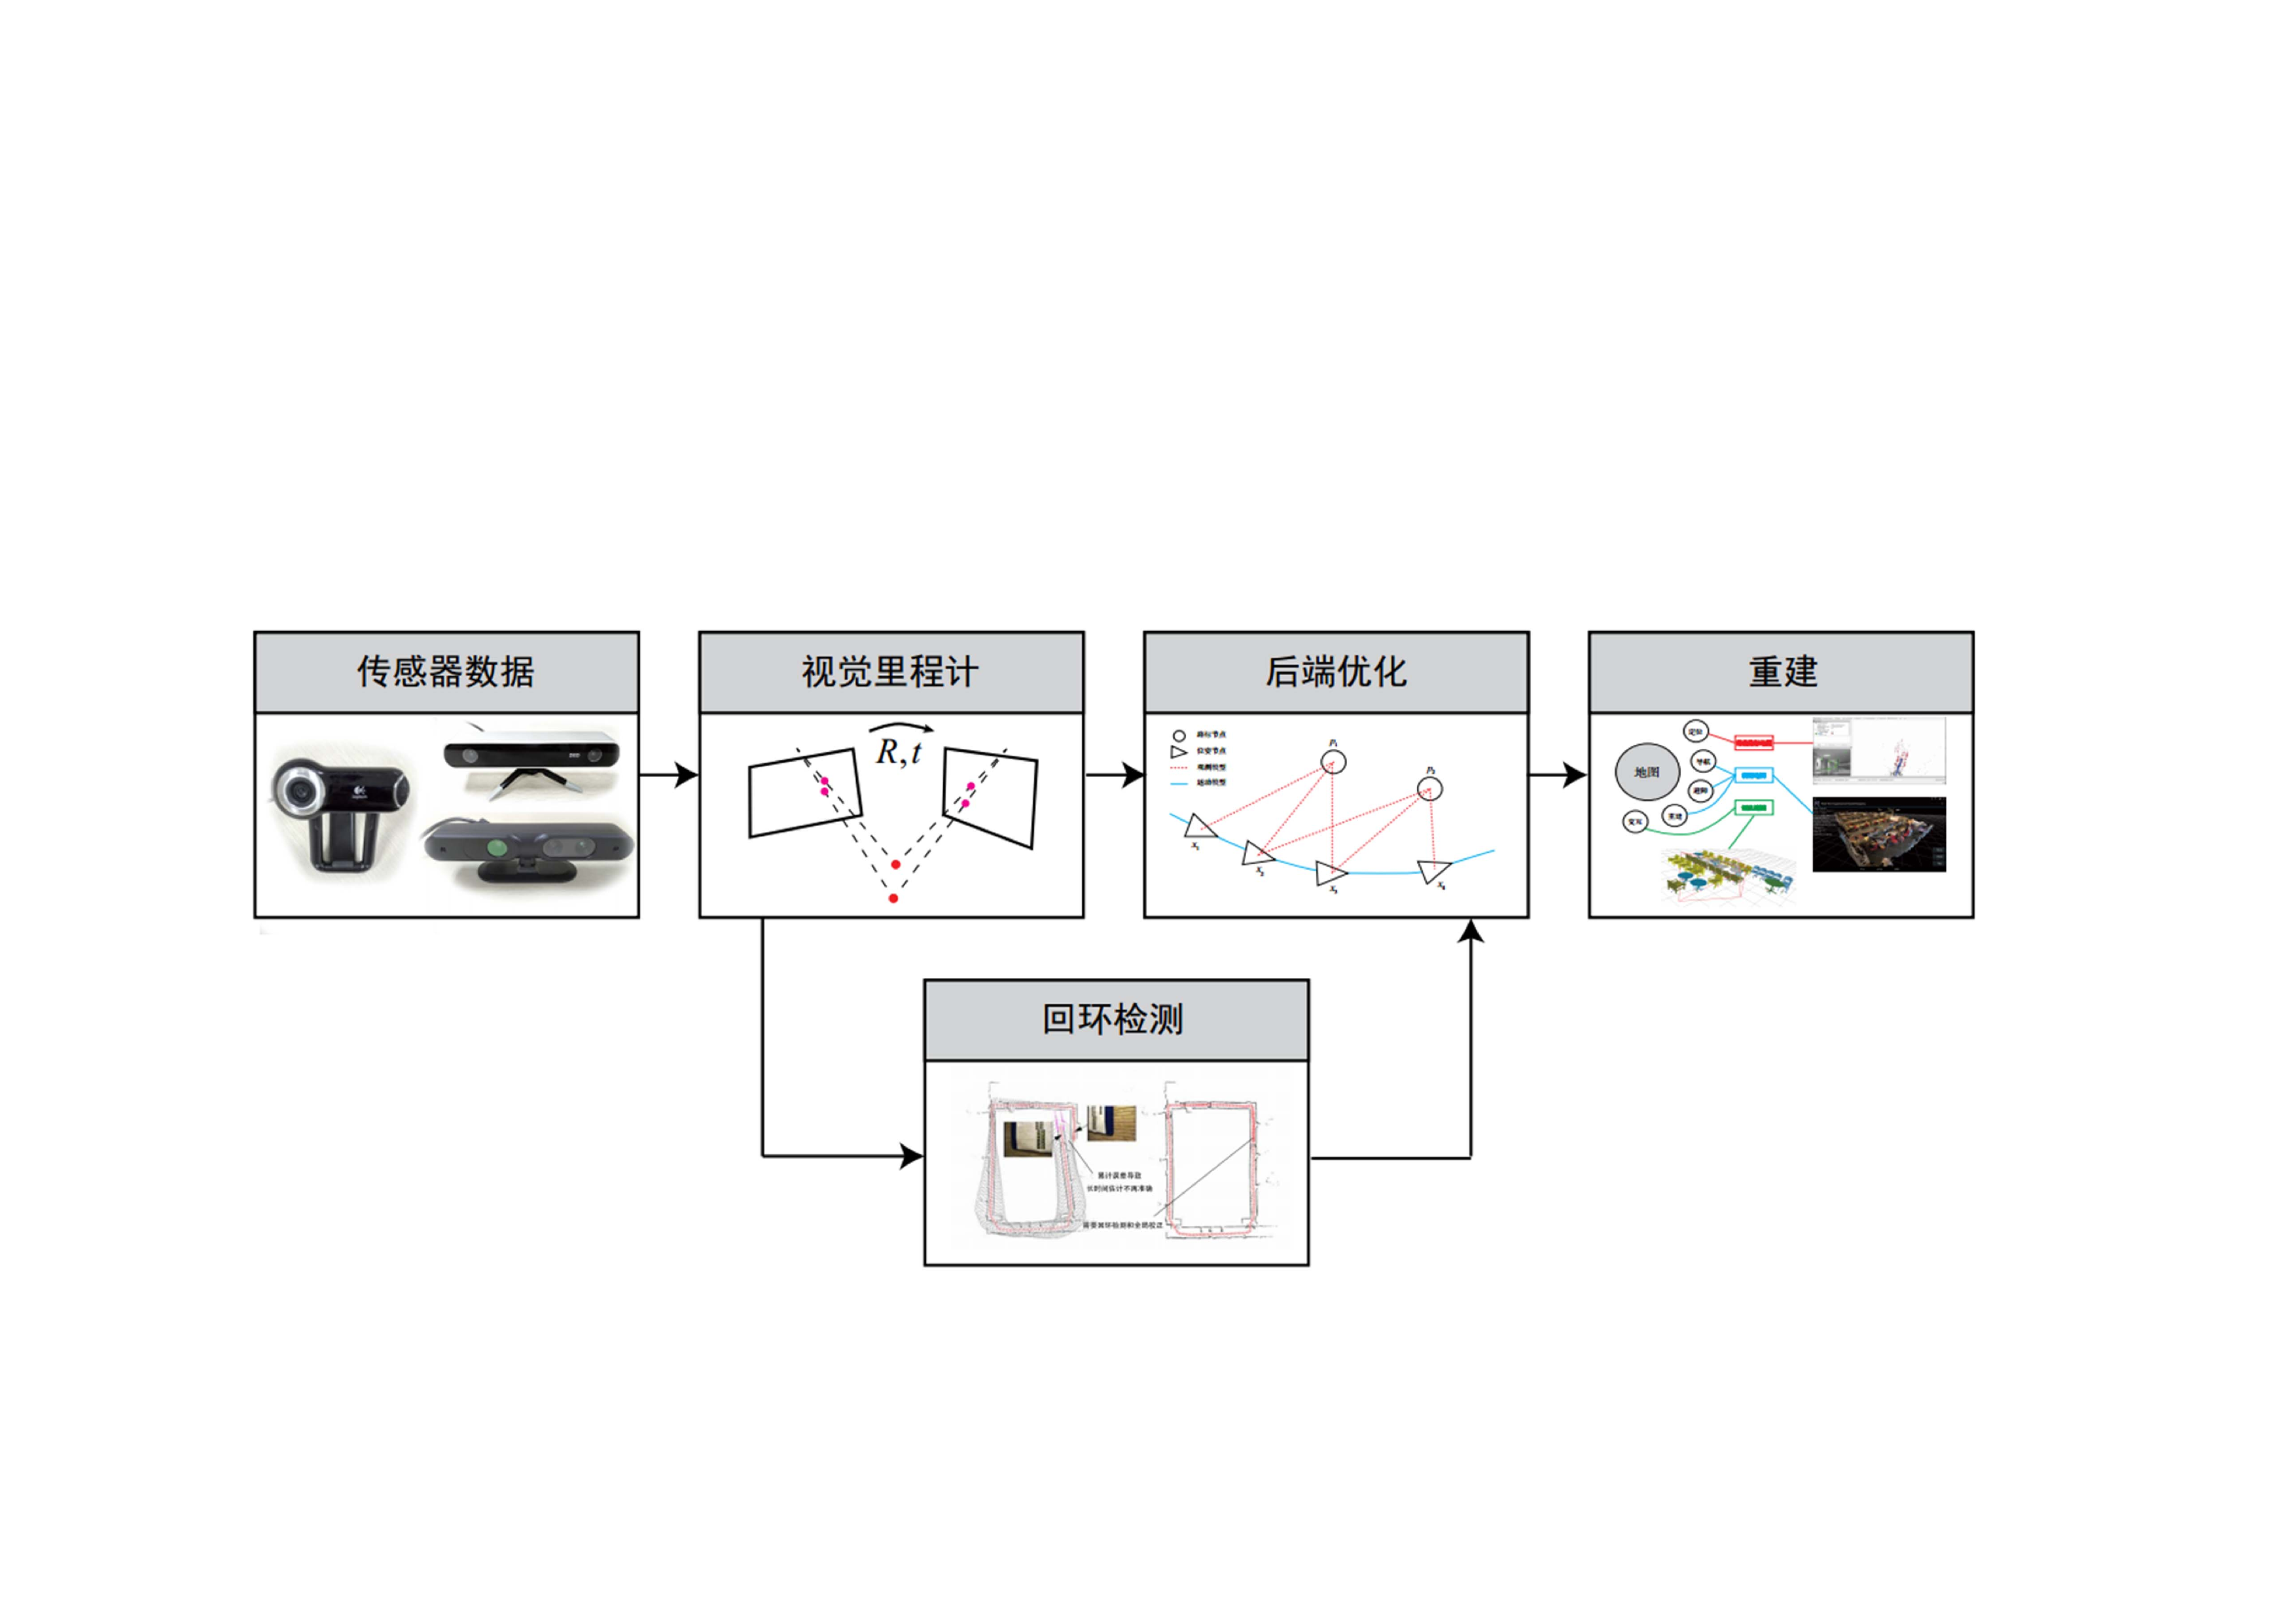
\includegraphics[scale=0.3,angle=-90]{figures/Fig3-1.pdf}
\caption{视觉SLAM算法框架}
\label{fig3.1}
\end{figure}

%3.1.1
\subsection{视觉里程计}
SLAM是一个状态估计问题,然而实际的传感器输出大都很难直接作为状态估计模型的输入。因而视觉里程计的主要任务是根据传感器输入,估计图像$I_i \rightarrow I_j$的相对位姿$T_ij$,串联相对位姿并三角化观测到的地图点得到运动轨迹与局部地图,将图像数据抽象为适于估计的数学模型。视觉里程计一般只估计相邻时刻的运动,和再过往的状态没有关联。视觉里程计主要包括两个部分,传感器数据关联和运动估计,其算法流程如图\ref{fig3.2}所示。根据视觉里程计传感器关联数据方式的不同,当前主流SLAM算法分为基于直接法和基于特征的SLAM算法,具体原理将在3.2节中详细介绍。

\begin{figure}[h]
\centering
%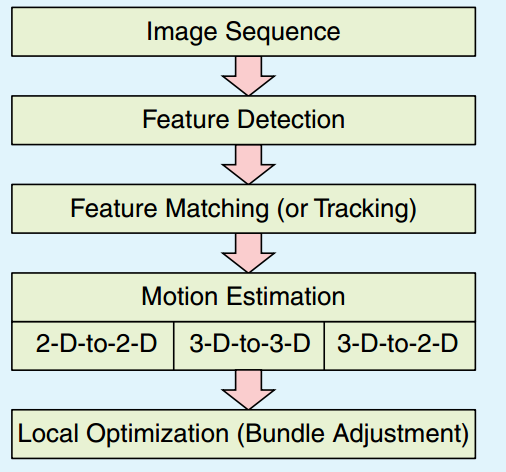
\includegraphics[scale=0.5]{figures/Fig3.2.png}
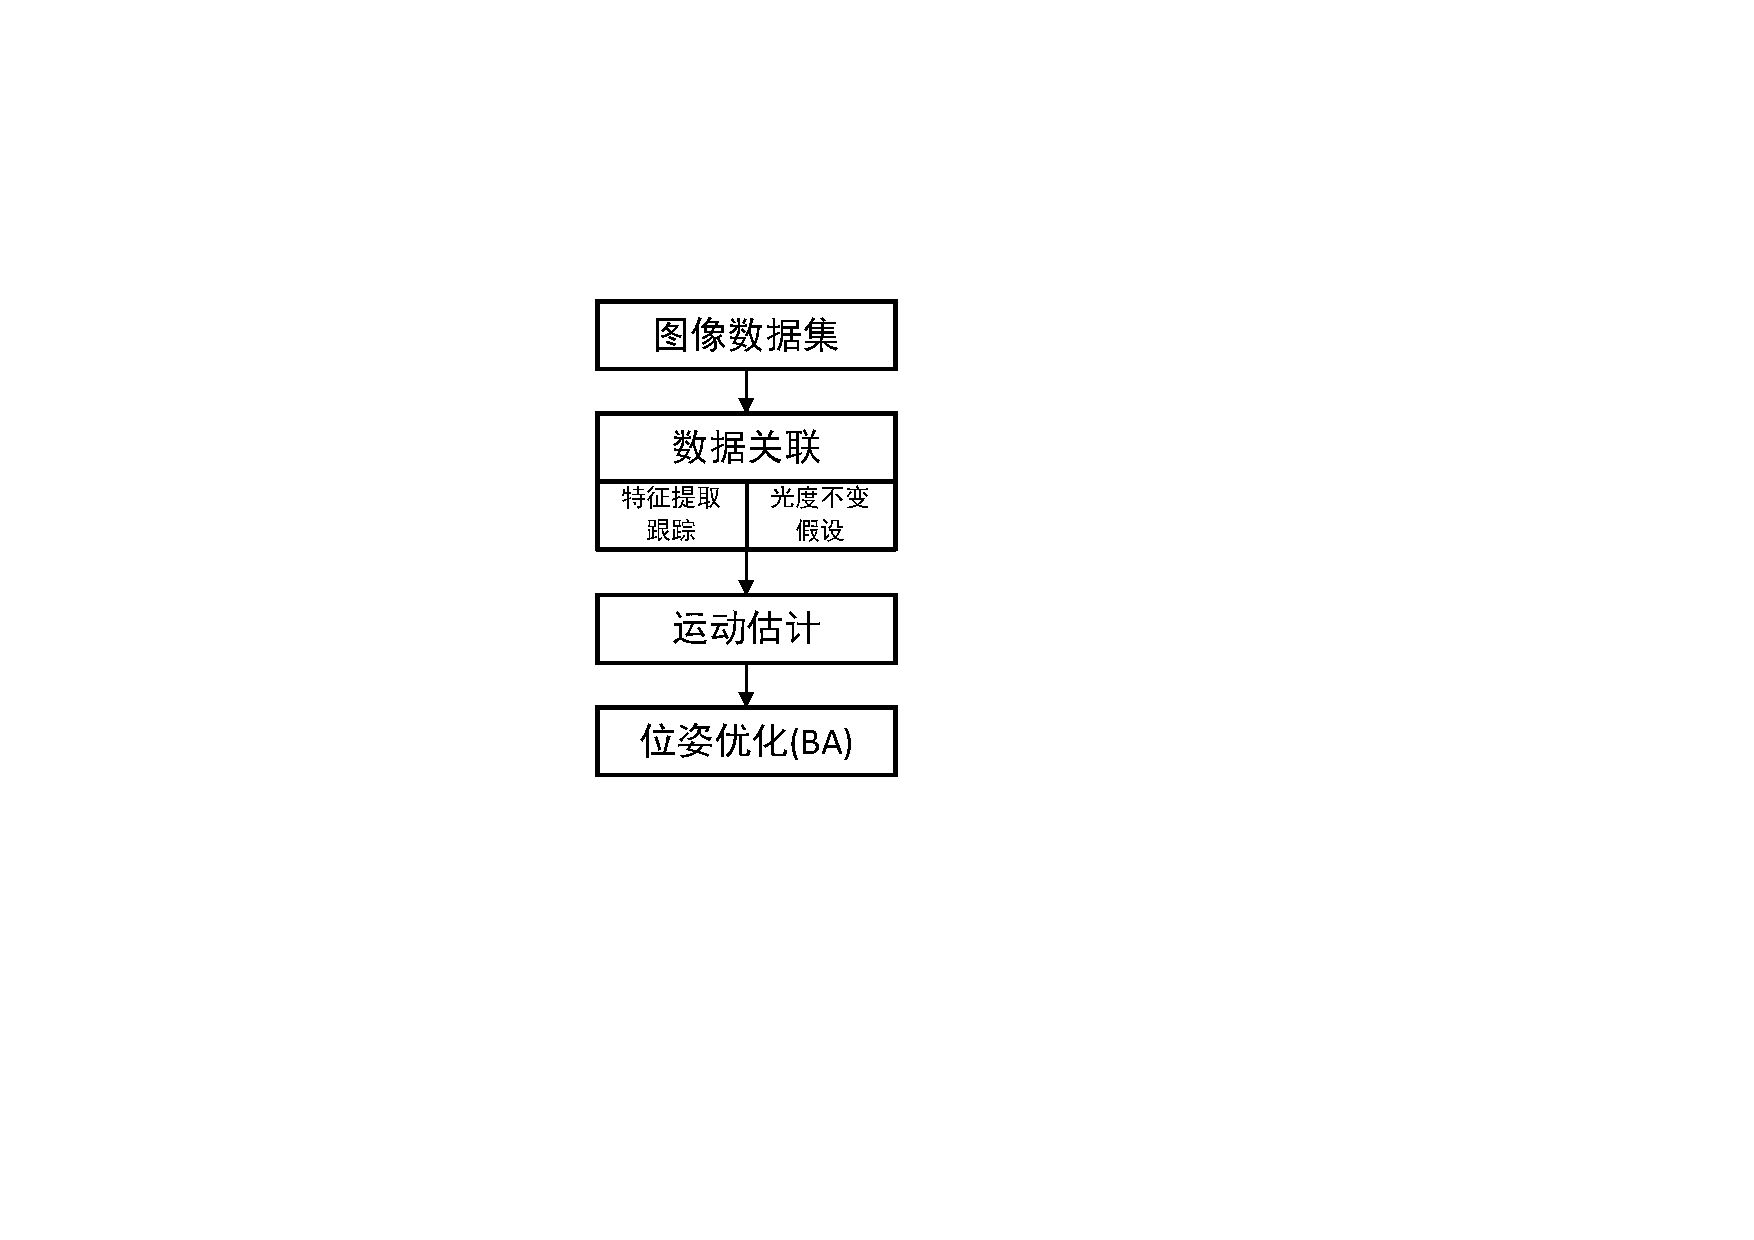
\includegraphics[scale=0.7,angle=-90]{figures/Fig3-2.pdf}
\caption{视觉里程计算法流程图}
\label{fig3.2}
\end{figure}

视觉里程计得到的轨迹和地图,由于在运动估计时只考虑了帧间的信息,每次估计都带有一定的误差,串联的轨迹无可避免会出现累计漂移,这将导致无法得到全局一致的轨迹与地图。需要通过后端优化算法进行处理,估计运动和周围环境空间的不确定性,减小估计误差,提高轨迹和地图的一致性。


%3.1.2
\subsection{后端优化}
SLAM算法的后端优化将SLAM问题看作最大后验概率估计问题,且大都采用因子图的方式来推到变量之间的以来关系。一般的,假设代估计状态变量为$\mathcal{X}$,在SLAM中变量$\mathcal{X}$包括无人机的轨迹和地图点的位置。传感器可以获得一组测量值$Z=\lbrace z_k:k=1,\ldots ,m\rbrace$,且每个测量值可以表示为状态变量$\chi$的函数,例如$z_k=h_k\left( \mathcal{X}_k \right)+\epsilon_k$,其中$\mathcal{X}_k \in \mathcal{X}$是变量的子集,$h_k(\cdot)$表示传感器的观测模型,$\epsilon_k$是随机观测误差。

在最大后验概率估计中,通过计算变量$\mathcal{X}^*$的概率分布来估计状态变量$\mathcal{X}$,$\mathcal{X}^*$表示最大后验概率$\mathds{P}\left(\mathcal{X} \vert Z\right)$:
\begin{equation}
\label{equ3.1}
\mathcal{X}^* 
\doteq 
\argmax \limits_{\mathcal{X}} \mathds{P}\left(\mathcal{X} \vert Z\right) 
=
\argmax \limits_{\mathcal{X}}\mathds{P}\left(Z \vert \mathcal{X}  \right)\mathds{P}\left(\mathcal{X}\right)
\end{equation}
上式推导来源于贝叶斯定义。在公式\eqref{equ3.1}中,$\mathds{P}\left(Z \vert \mathcal{X}  \right)$表示在状态变量$\mathcal{X}$分布确定情况下测量值$Z$的似然,$\mathds{P}\left(\mathcal{X}\right)$表示状态$\mathcal{X}$的先验概率。先验概率包括任何关于状态$\mathcal{X}$的先验信息,如果没有可用的先验信息,则$\mathds{P}\left(\mathcal{X}\right)$表示为一个常亮从而可以从优化过程中移除。在这种情况下,最大后验概率可以简化为极大似然估计。

假设测量值$Z=\lbrace z_k:k=1,\ldots ,m\rbrace$相互独立(影响测量的噪声是不相关的),公式\eqref{equ3.1}可以因式分解为:
\begin{equation}
\label{equ3.2}
\mathcal{X}^* 
\doteq 
\argmax \limits_{\mathcal{X}} \mathds{P}\left(\mathcal{X}\right) \prod \limits_{k=1}^{m} \mathds{P}\left(z_k \vert \mathcal{X}  \right)
=
\mathds{P}\left(\mathcal{X}\right) \prod \limits_{k=1}^{m} \mathds{P}\left(z_k \vert \mathcal{X}_k  \right)
\end{equation}
其中,等式右边的测量值$z_k$仅仅与状态变量$\mathcal{X}_k$的子集有关。

公式\eqref{equ3.2}可以因子图表示。待估计的状态变量用节点表示,似然$\mathds{P}\left(z_k \vert \mathcal{X}_k  \right)$和先验$\mathds{P}\left(\mathcal{X} \right)$由因子表示,因子建立了对节点子集的概率约束。因子图是一种建立第$k$个因子和对应状态变量$\mathcal{X}_k$依赖关系的图模型。因子图可以将SLAM问题可视化,便于理解,SLAM算法的因子图描述如图\ref{fig3.3}表示。

\begin{figure}
\centering
%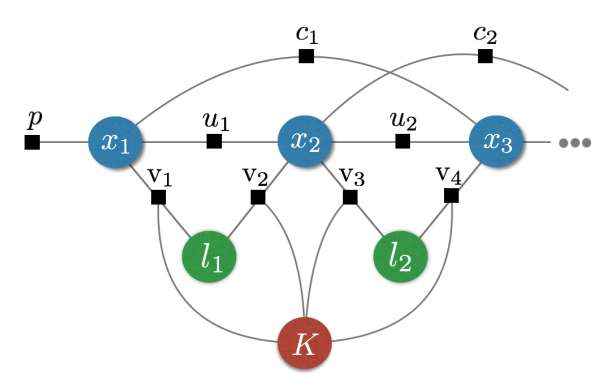
\includegraphics[scale=0.5]{figures/Fig3.3.png}
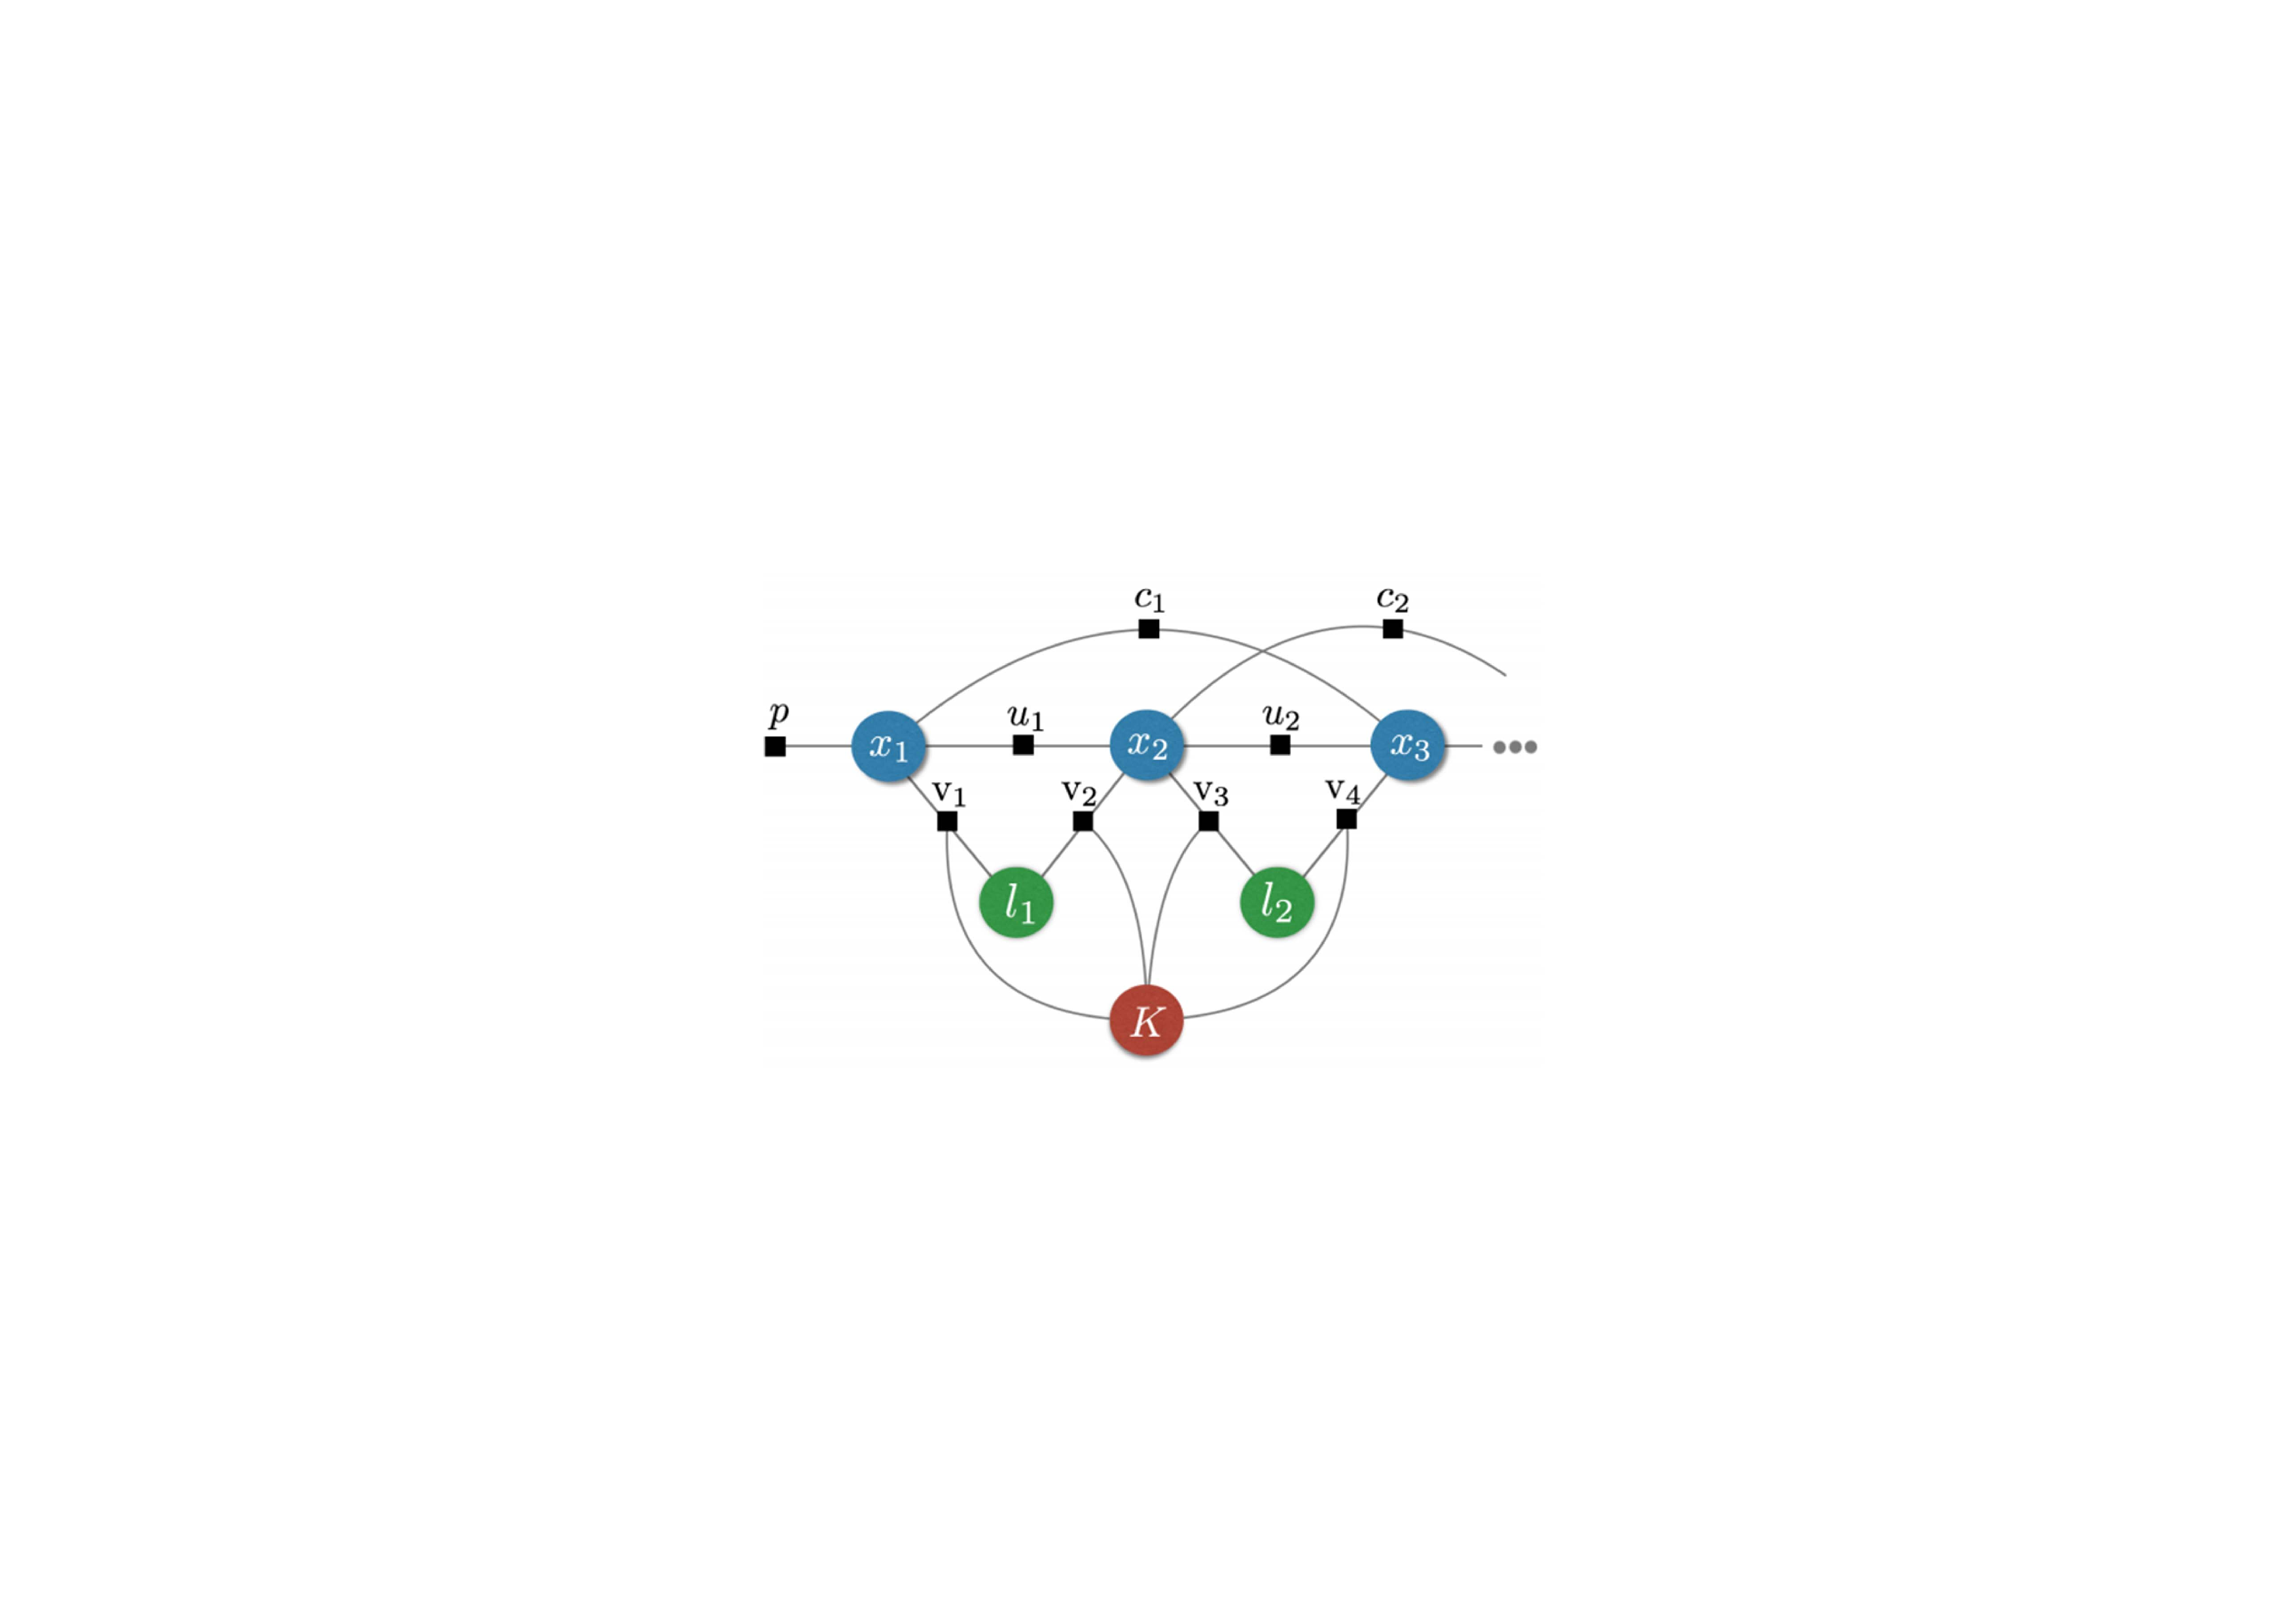
\includegraphics[scale=0.5,angle=-90]{figures/Fig3-3.pdf}
\caption{SLAM因子图}
\label{fig3.3}
\end{figure}


为了更清楚的表示公式\eqref{equ3.2},假设观测模型的测量噪声$\epsilon_k$服从信息矩阵为$\Omega_k$的0均值高斯分布。测量值的似然可以表示为
\begin{equation}
\label{equ3.3}
\mathds{P}\left(z_k \vert \mathcal{X}_k  \right) \varpropto \exp ( -{1 \over 2} \left\| h_k\left( \mathcal{X}_k \right) - z_k \right\|_{\Omega_k}^2 )
\end{equation}
其中,使用符号$\left\| e \right\|_{\Omega}^2 = e^T \Omega e$。类似的,假设先验也服从高斯分布:
\begin{equation}
\label{equ3.4}
\mathds{P}\left( \mathcal{X}_k  \right) \varpropto \exp ( -{1 \over 2} \left\| h_0\left( \mathcal{X}_0 \right) - z_0 \right\|_{\Omega_0}^2 )
\end{equation}
其中$h_0(\cdot)$表示观测模型,先验均值为$z_0$,信息矩阵为$\Omega_0$。由于最大后验与最小负对数后验等价,则公式\eqref{equ3.2}的最大后验估计可以表示为:
\begin{equation}
\label{equ3.5}
\mathcal{X}^* 
=
\argmin \limits_{\mathcal{X}} - \log \left( \mathds{P}\left(\mathcal{X}\right) \prod \limits_{k=1}^{m} \mathds{P}\left(z_k \vert \mathcal{X}_k  \right) \right)
=
\argmin \limits_{\mathcal{X}} \sum \limits_{k=0}^{m} -{1 \over 2} \left\| h_k\left( \mathcal{X}_k \right) - z_k \right\|_{\Omega_k}^2
\end{equation}
公式\eqref{equ3.5}的形式是典型的非线性最小二乘问题,其中$h_k{\cdot}$是一个非线性函数。需要注意的是,公式\eqref{equ3.5}推导的前提是假设观测模型的观测噪声服从高斯分布。对于不同的观测噪声分布,将会得到不同的优化目标函数。例如,若观测噪声服从拉普拉斯分布,则公式\eqref{equ3.5}的平方$l_2$范数应变为$l_1$范数。为了增加算法对于离群点的鲁棒性,通常使用鲁棒核函数替换公式\eqref{equ3.5}中的平方$l_2$范数。

公式\eqref{equ3.5}的形式与运动结构学中的Bundle Adjustment(BA)问题相似。这是因为公式\eqref{equ3.5}与BA都是从最大后验概率估计出发推导得到的。但是,SLAM问题具有两个特点。首先,不同于BA问题受限于几何模型约束,公式\eqref{equ3.5}适用于各种传感器模型。比如惯性传感器,GPS,轮式传感器等。其次,公式\eqref{equ3.5}是增量式的求解,在无人机运动时,可以获得新的观测值。

对于解决公式\eqref{equ3.5}的最小化问题,可通过连续线性化进行求解。例如高斯-牛顿法(G-N)和列文伯格-马夸尔特法(L-M)。高斯-牛顿方法从初始估计给定的初值$\hat{\mathcal{X}}$开始迭代,每次迭代时高斯-牛顿法估计公式\eqref{equ3.5}的最小值
\begin{equation}
\label{equ3.6}
\delta_\mathcal{X}^* 
=
\argmin \limits_{\delta_\mathcal{X}} {1 \over 2} \sum \limits_{k=0}^{m} \left\| A_k\delta_\mathcal{X}-b_k \right\|_{\Omega_k}^2
=
\argmin \limits_{\delta_\mathcal{X}} {1 \over 2} \left\| A_k\delta_\mathcal{X}-b \right\|_{\Omega}^2
\end{equation}
其中公式\eqref{equ3.6}中的$\delta_\mathcal{X}$表示初始估计状态$\hat{\mathcal{X}}$的微小修正量。$A_k \doteq {\partial h_k(\mathcal{X}) \over \partial \mathcal{X}} $是观测模型$h_k(\cdot)$关于$\mathcal{X}$的雅各比,$b_k \doteq z_k-h(\mathcal{X})$表示测量值与观测模型输出的残差;公式\eqref{equ3.6}右边的矩阵$A$,$b$是由$A_k$,$b_k$组成的矩阵;$\Omega$是由观测噪声信息矩阵$\Omega_k$组成的对角块矩阵。

最小化公式\eqref{equ3.6}对应的微小修正$\delta_\mathcal{X}^* $可以用下面的闭型公式计算
\begin{equation}
\label{equ3.7}
\delta_\mathcal{X}^* = - \left( A^T \Omega A \right)^{-1} A^T \Omega b
\end{equation}
每次通过$\hat{\mathcal{X}} \leftarrow \hat{\mathcal{X}}+\delta_\mathcal{X}^*$迭代更新估计状态,矩阵$A^T \Omega A$称为Hessian矩阵。之前的推导过程中,我们假设$\mathcal{X}$属于向量空间。如果$\mathcal{X}$属于光滑的流形空间(如旋转),则高斯-牛顿法的形式保持不边,但是迭代更新方程$\hat{\mathcal{X}} \leftarrow \hat{\mathcal{X}}+\delta_\mathcal{X}$会被更合适的映射法则取代。在机器人领域中,通常使用符号$\oplus$表示状态更新的映射关系,并且将状态的微小修正量$\delta_\mathcal{X}$定义在流形状态变量$\hat{\mathcal{X}}$的切空间上,此时的更新方程为$\hat{\mathcal{X}}  \leftarrow \hat{\mathcal{X}} \oplus \delta_\mathcal{X}$。

现代SLAM算法最大的进步,在于认识到公式\eqref{equ3.7}中的雅各比矩阵$A$的稀疏性,而矩阵$A$的稀疏性是由于因子图内在的拓扑逻辑所决定的,这可以利用线性方法快速求解估计状态的微小增量$\delta_\mathcal{X}^*$。此外,利用矩阵$A$的稀疏性可以设计增量式的求解方法,将更新后的状态变量作为新的观测值。当前主流SLAM后端优化库(如GTSAM,g2o,Ceres,iSAM,SLAM++)可以在几秒之内求解数以万计的状态变量。

目前,通常使用最大后验估计,因子图优化,图优化,完全平滑和平滑映射来描述SLAM问题。其中特别需要介绍的描述方法是位姿图优化,位姿图中的状态变量是无人机运动中的采样位姿,约束是两位姿之间的相对运动约束。

%3.1.3
\subsection{回环检测}
前两节介绍了前端视觉里程计和后端优化:前端将传感器观测到的数据进行关联并将数据抽象为适于后端估计的数据(轨迹,地图点位置);后端负责根据前端的结果对系统状态进行优化。然而,前端的视觉里程计只考虑时间关联性,之前测量产生的误差不可避免的会累计到下一时刻,使得SLAM出现累计误差,无法构建权全局一致的轨迹和地图。后端优化虽然能够估计最大后验误差,但由于前端只提供了相邻时刻关键帧数据,无法消除累计误差。回环检测又称闭环检测,负责检测传感器是否经过同一个位置,通过增加窗时间下的数据关联性约束,消除SLAM的轨迹与地图随时间漂移而产生的累计误差。回环检测对于SLAM算法意义重大,关系到SLAM算法估计的轨迹和地图在长时间下的准确性。另外,由于回环检测可以提供当前数据与历史数据的关联性,当SLAM算法前端跟踪失效丢失后,可以利用回环检测进行重定位,有效提高整个SLAM算法的精度和鲁棒性。

常用的回环检测方法有两种:基于里程计的几何关系或基于外观的图像间相似性。基于里程计的几何方法利用视觉里程计的位置信息,当发现运动到之前的某个位置附近时检测是否有回环关系。这是一种很直接的检测思路,但是由于存在累计误差,里程计无法正确的发现到是否回到了曾经的某个位置。另一种方法是基于外观的,这种方法和前端后端的输出都无关,仅仅根据两幅图像之间的相似性进行判断。这种方法与累计误差完全无关,可以独立作为SLAM算法的一个模块,成为视觉SLAM中的主流算法,应用与多个实际的系统中。


%3.2
\section{主流单目视觉SLAM算法研究}
近些年出现了许多优秀的单目SLAM算法理论,按照前端视觉里程计关联数据的方式不同主要分为基于直接法的SLAM算法和基于特征的SLAM算法两种。基于直接法SLAM算法假设同一空间点的像素灰度值在不同图像中固定不变,估计最优位姿使得两幅图像经变换后灰度变化最小,完成前端的数据关联。基于特征的SLAM算法则提取图像中的特征,并在不同图像间对相同特征进行匹配,从而解算图像之间的相对运动,关联前端数据。本节主要研究两种具有代表性的单目SLAM算法:LSD-SLAM和ORB-SLAM。分析两算法的原理、优势和不足,针对单目SLAM算法存在的不足提出改进方向。

%3.2.1
\subsection{基于直接法的LSD-SLAM}


\subsubsection*{算法概述}
LSD-SLAM是2014年慕尼黑工业大学的J.Engle等人提出的基于直接法的SLAM算法,无需计算图像特征点,通过直接法的像素关联估计运动状态,构建半稠密地图——这里的半稠密是指估计灰度梯度明显区域的像素位置。该算法可以在大尺度环境下实时运行,利用半稠密像素关联和关键帧pose图构建全局一致的地图,关键帧间的约束pose图使用相似变换$\mathfrak{sim}(3)$代替$\mathfrak{se}(3)$显示的表示尺度,从而在后端优化中可以考虑不同场景的尺度,减小尺度漂移。LSD-SLAM算法的流程如图\ref{fig3.4}所示

\begin{figure}
\centering
%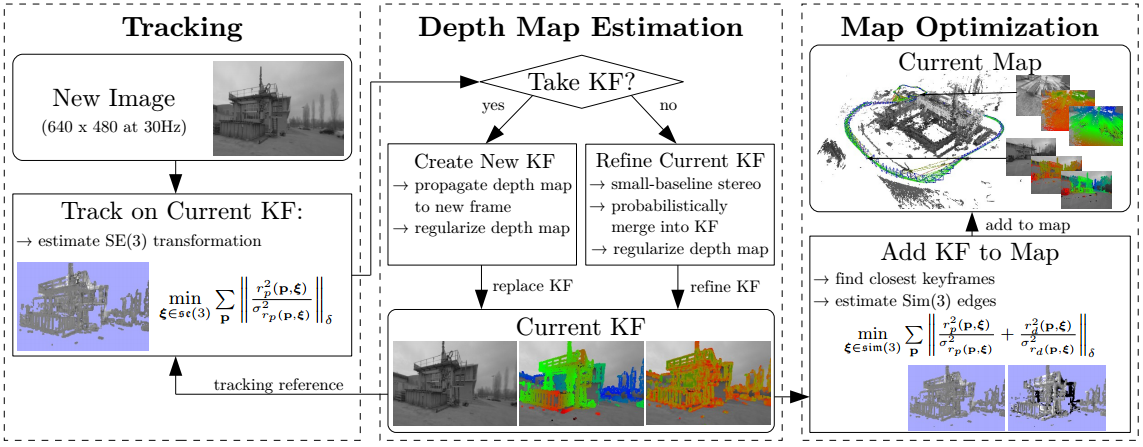
\includegraphics[scale=0.35]{figures/Fig3.4.png}
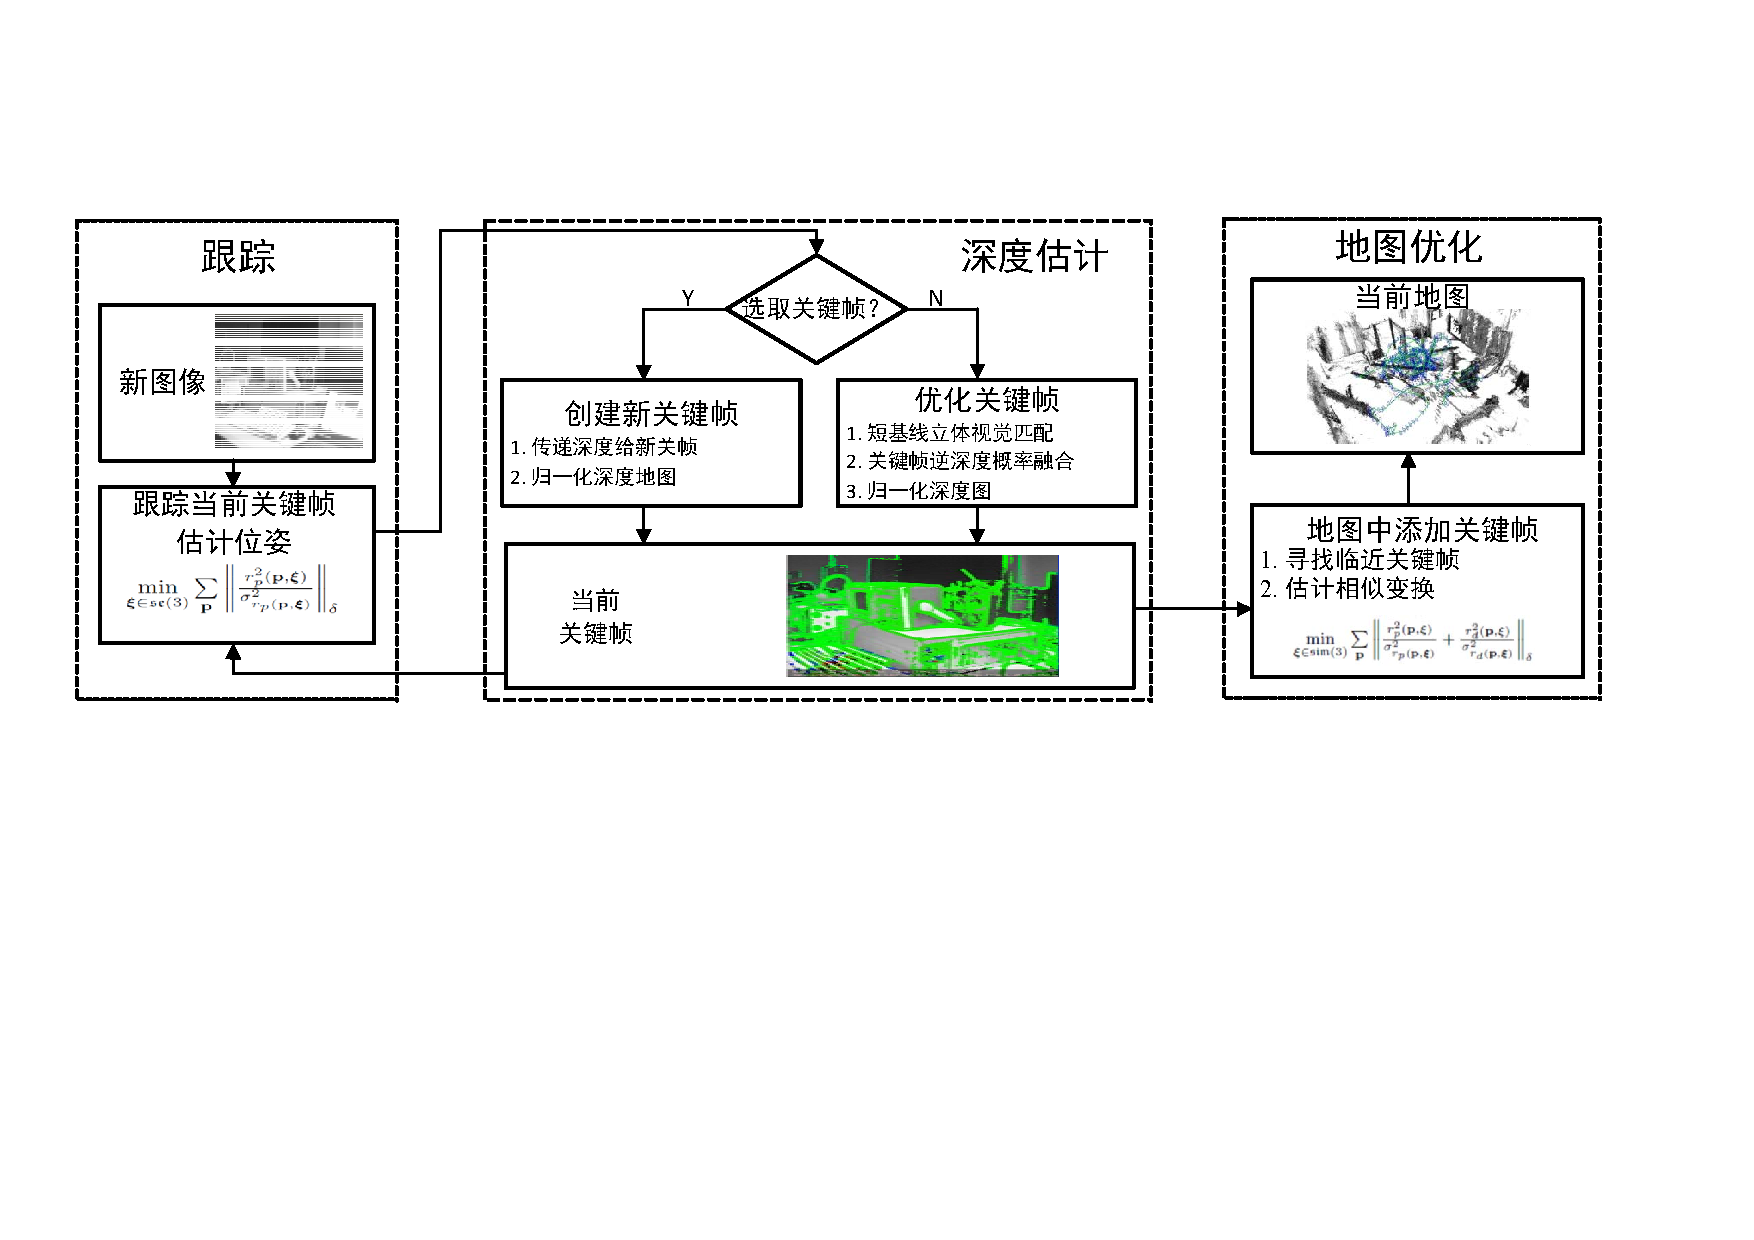
\includegraphics[scale=0.5,angle=-90]{figures/Fig3-4.pdf}
\caption{LSD-SLAM算法流程图\upcite{}}
\label{fig3.4}
\end{figure}

LSD-SLAM算法主要分为三个模块:图像跟踪,地图深度估计和地图优化。图像跟踪模块获取传相机采集的图像,利用上一帧的图像位姿作为初值,估计当前帧相对于关键帧的相对位姿$\xi \in \mathfrak{se}(3) $;地图深度估计模块根据前帧情况,进行关键帧替换或优化当前关键帧的位姿和地图点深度。如果相机运动过快,则将新关键帧的地图点投影到临近关键帧进行初始化;如果当前帧被创建为新的关键帧,则之前的关键帧的深度不再被优化。地图优化模块将之前的关键帧加入到全局地图中,使用尺度感知和相似变换图像关联来检测回环和尺度漂移,估计相邻关键帧之间的相似变换$\xi \in \mathfrak{sim}(3)$优化关键帧的位姿和深度。

\subsubsection*{数据关联与运动估计}
基于直接法的SLAM算法的前提是灰度不变假设,即认为同一空间点的像素灰度值,在不同图像中保持不变。直接法预先不知道单个像素与像素间的对应关系,而是通过最小化光度误差来求解位姿变换和对应关系。如图\ref{fig3.5}所示,空间某点P和两时刻图像上的对应像素点。空间点P的世界坐标为$[X,Y,Z]^T$,内参为$\boldsymbol{K}$的两相机对应的像素坐标为$\boldsymbol{p_1},\boldsymbol{p_2}$。为了估计从相机1到相机2的相对位姿,以相机1为参考系假设相机2的位姿为$\boldsymbol{R},\boldsymbol{t}$,对应的李代数为$\boldsymbol{\xi}$。根据相机投影模型有:
\begin{equation}
\label{equ3.8}
\begin{aligned}
& \boldsymbol{p_1} = 
\begin{bmatrix}
u_1 \cr v_1 \cr 1 \cr 
\end{bmatrix}
={1 \over Z_1} \boldsymbol{K} \boldsymbol{P}
\\
& \boldsymbol{p_2} = 
\begin{bmatrix}
u_2 \cr v_2 \cr 1 \cr
\end{bmatrix}
={1 \over Z_2} \boldsymbol{K} ( \boldsymbol{R} \boldsymbol{P}+\boldsymbol{t}) = {1 \over Z_2} \boldsymbol{K} ( \exp (\boldsymbol{\xi}^{\wedge}) \boldsymbol{P})_{1:3}
\end{aligned}
\end{equation}
其中$Z_1$,$Z_2$是空间点P在两个相机坐标系下的深度,$(\cdot)^{\wedge}$表示向量的反对称矩阵。由于位姿$\exp(\boldsymbol{\xi}^{\wedge})$应该与齐次坐标相乘,得到的结果只取前三个元素。

\begin{figure}
\centering
%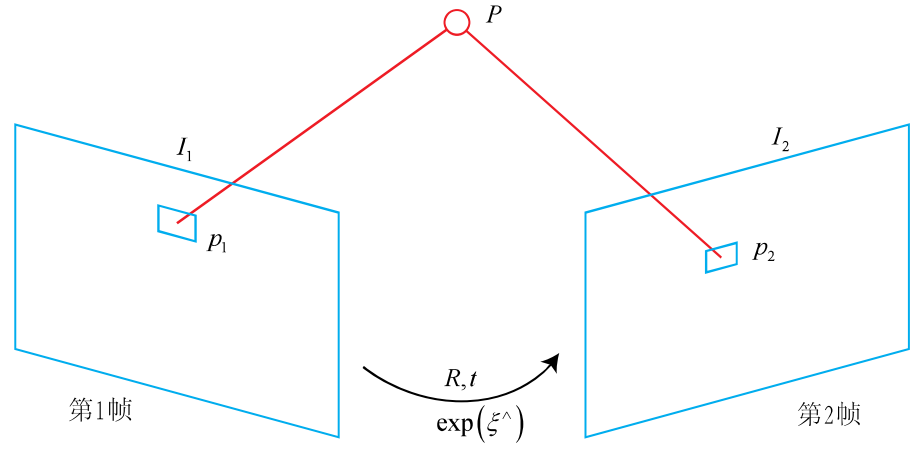
\includegraphics[scale=0.5]{figures/Fig3.5.png}
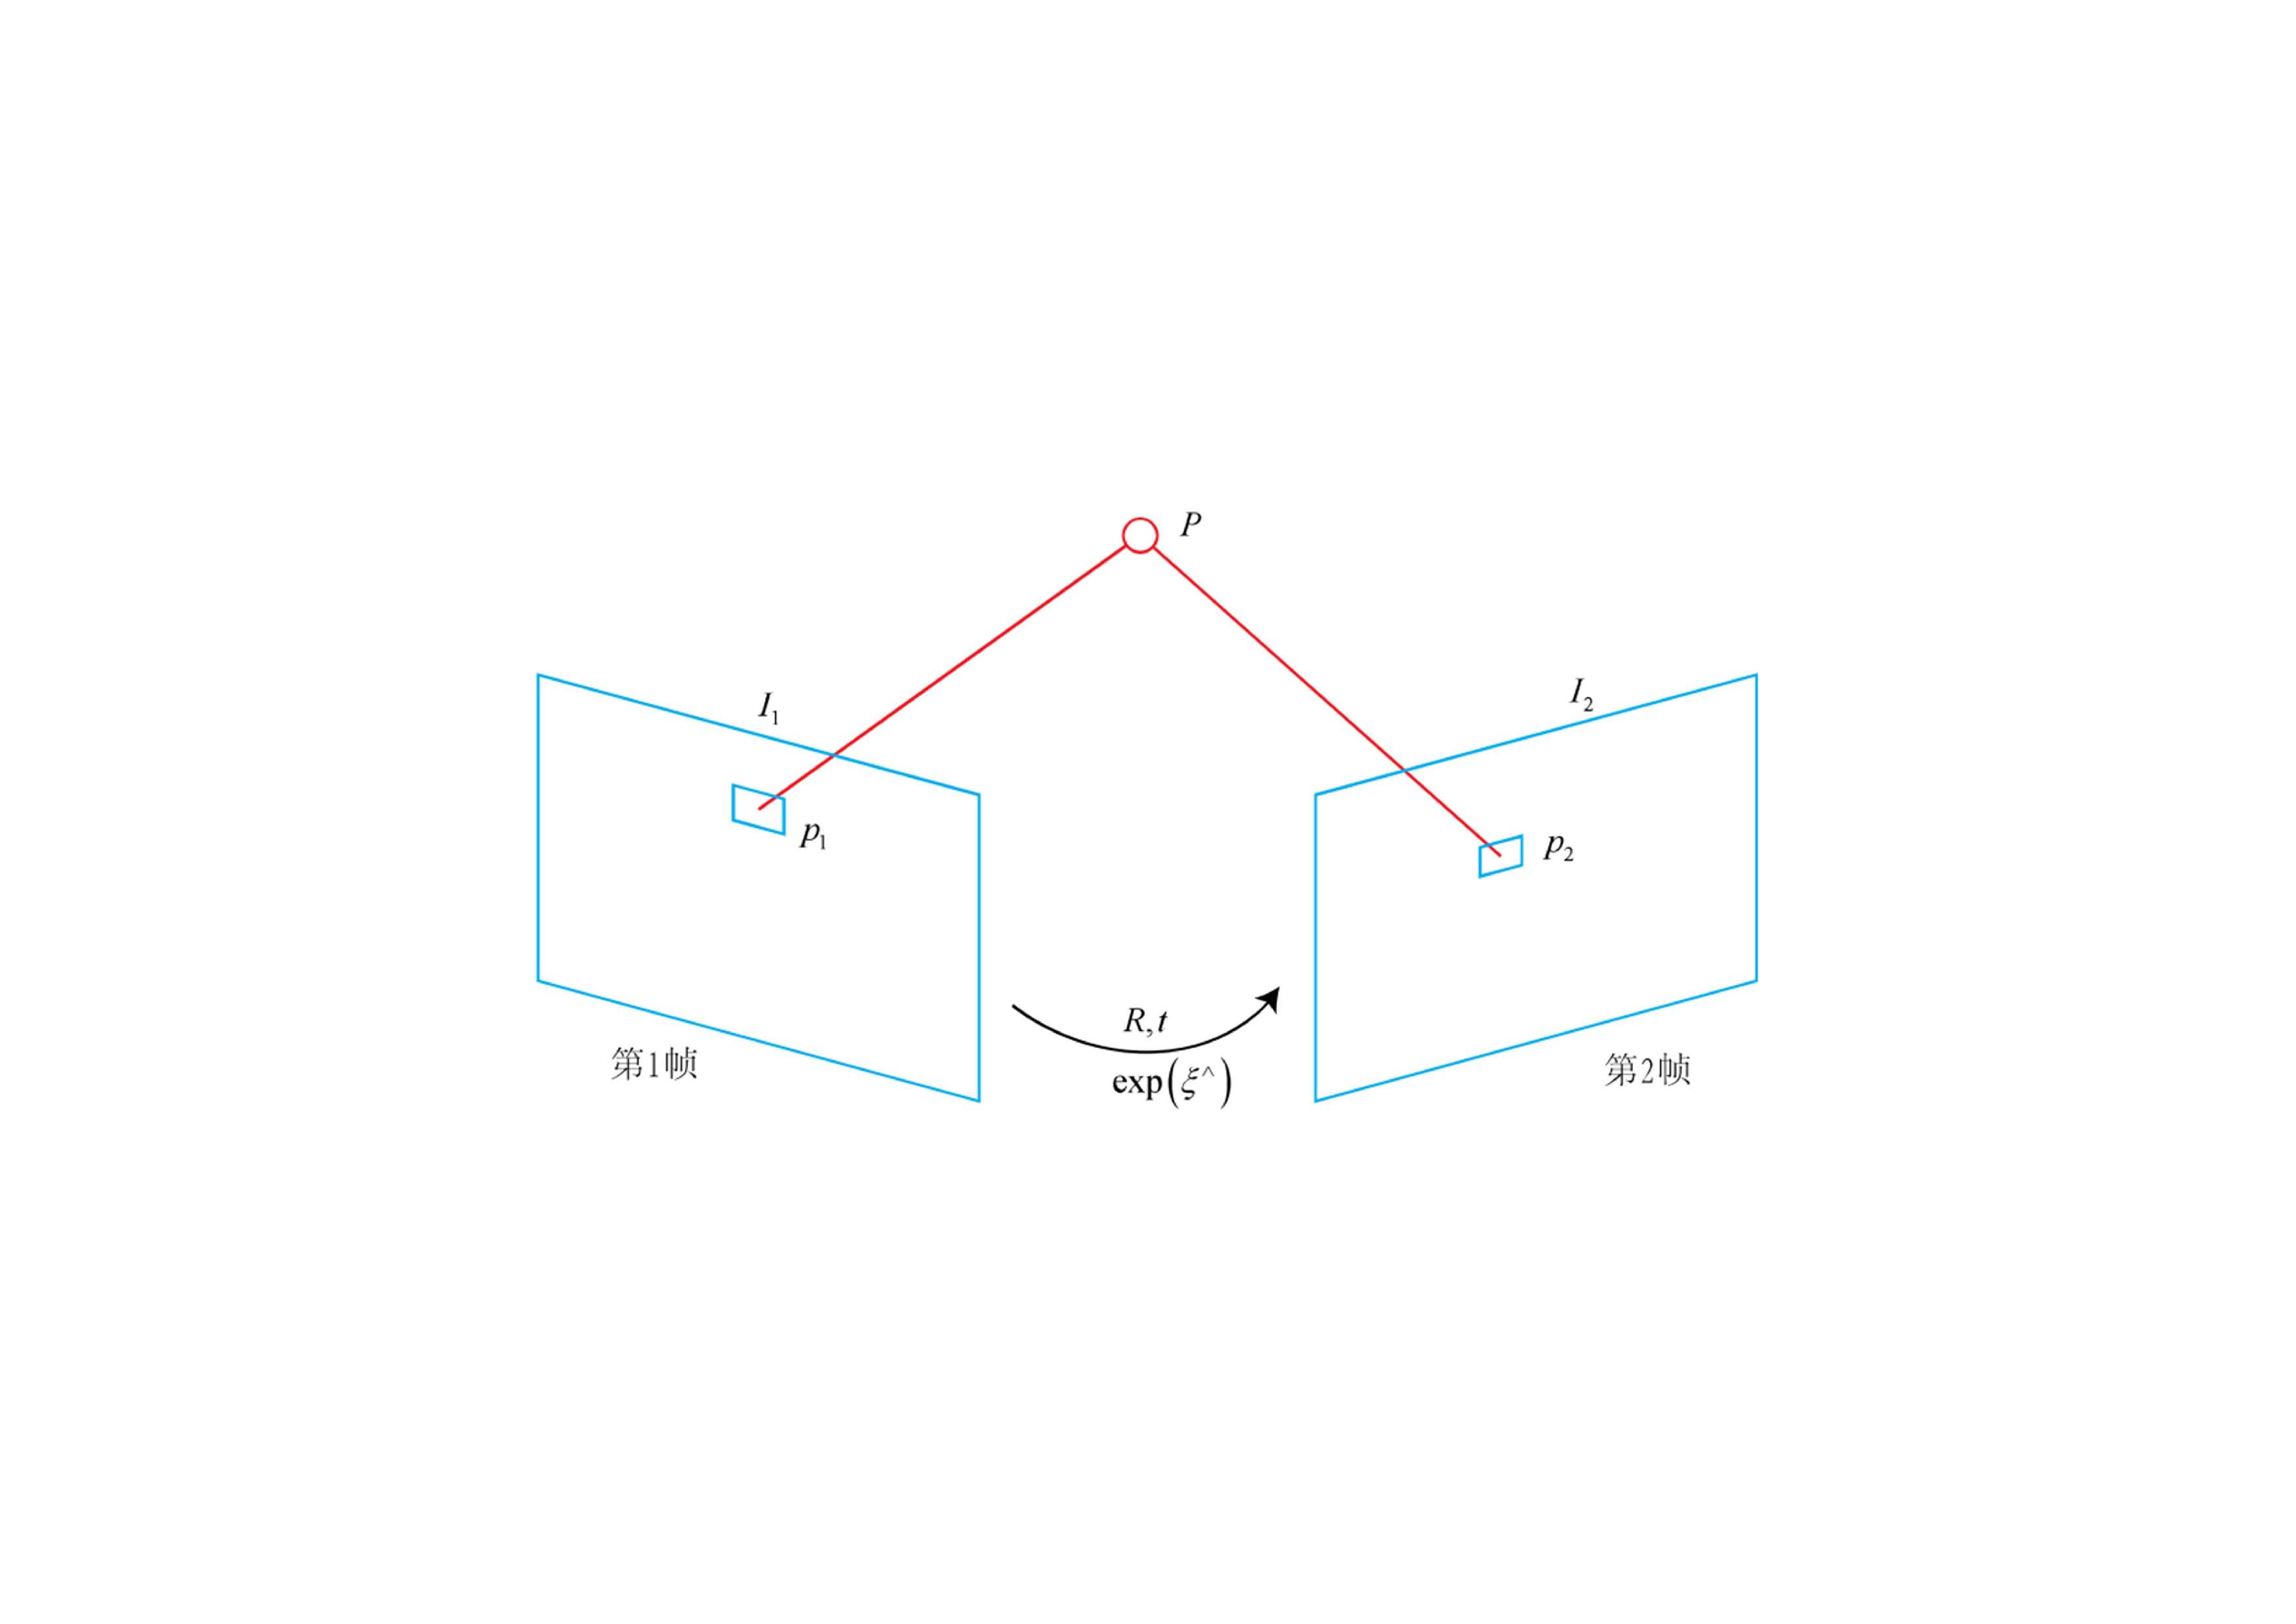
\includegraphics[scale=0.35,angle=-90]{figures/Fig3-5.pdf}
\caption{直接法示意图}
\label{fig3.5}
\end{figure}

直接法中只已知像素的灰度值,无法直接提供两幅图像的像素匹配,而是根据灰度不变假设估计相机间的相对位姿,最小化两幅图像像素之间的光度误差,也就是$P$点对应两个像素点的灰度误差。
\begin{equation}
\label{equ3.9}
\begin{aligned}
& e = I_1(\boldsymbol{p}_1) - I_2(\boldsymbol{p}_2) 
\\ 
& \min\limits_{\boldsymbol{\xi}} J(\boldsymbol{\xi}) = \Vert e \Vert ^2
\end{aligned}
\end{equation}
其中$I(\cdot)$表示图像像素灰度函数,目标优化函数为误差的二范数。对于空间中所有空间点,都应该满足灰度不变假设。若存在$N$个空间点$P_i$,则相机位姿估计问题可以表示为
\begin{equation}
\label{equ3.10}
\min\limits_{\boldsymbol{\xi}} J(\boldsymbol{\xi}) = \sum\limits_{i=1}^N e_i^T e_i
\end{equation}
其中优化函数的优化变量是相机位姿$\boldsymbol{\xi}$,为了求解最优解需要研究位姿$\boldsymbol{\xi}$变化对误差$e$的影响,即误差关于位姿的导数。使用李代数左乘扰动模型给$\exp(\boldsymbol{\xi}^{\wedge})$增加扰动$\exp( \delta \boldsymbol{\xi}^{\wedge})$,有
\begin{equation}
\label{equ3.11}
\begin{aligned}
e(\boldsymbol{\xi}\oplus \delta \boldsymbol{\xi}) & = I_1\left({1 \over Z_1} \boldsymbol{K} \boldsymbol{P} \right) - I_2\left({1 \over Z_2} \boldsymbol{K} \exp (\delta \boldsymbol{\xi}^{\wedge}) \exp (\boldsymbol{\xi}^{\wedge}) \boldsymbol{P} \right)
\\
& \simeq I_1\left( {1 \over Z_1} \boldsymbol{K} \boldsymbol{P} \right) - I_2 \left( {1 \over Z_2} \boldsymbol{K} (1+\delta \boldsymbol{\xi}^{\wedge}) \exp (\boldsymbol{\xi}^{\wedge}) \boldsymbol{P} \right)
\\
& = I_1\left( {1 \over Z_1} \boldsymbol{K} \boldsymbol{P} \right) - I_2 \left({1 \over Z_2} \boldsymbol{K} \exp (\boldsymbol{\xi}^{\wedge}) \boldsymbol{P}+ {1 \over Z_2} \boldsymbol{K} \delta \boldsymbol{\xi}^{\wedge} \exp (\boldsymbol{\xi}^{\wedge}) \boldsymbol{P} \right)
\end{aligned}
\end{equation}
记公式\eqref{equ3.11}中的$\boldsymbol{q} = \delta \boldsymbol{\xi}^{\wedge} \exp (\boldsymbol{\xi}^{\wedge}) \boldsymbol{P} $,$\boldsymbol{u}={1 \over Z_1} \boldsymbol{K} \boldsymbol{P}$,$\boldsymbol{q}$为P点在扰动下的相机2坐标系下的坐标,$\boldsymbol{u}$为它的像素坐标。利用一阶泰勒近似,有
\begin{equation}
\label{equ3.12}
\begin{aligned}
e(\boldsymbol{\xi}\oplus \delta \boldsymbol{\xi}) &= I_1\left({1 \over Z_1} \boldsymbol{K} \boldsymbol{P} \right) - I_2 \left({1 \over Z_2} \boldsymbol{K} \exp (\boldsymbol{\xi}^{\wedge}) \boldsymbol{P}+ \boldsymbol{u} \right) 
\\ 
& \simeq I_1\left({1 \over Z_1} \boldsymbol{K} \boldsymbol{P} \right) - I_2 \left({1 \over Z_2} \boldsymbol{K} \exp (\boldsymbol{\xi}^{\wedge}) \boldsymbol{P} \right) - {\partial I_2 \over \partial \boldsymbol{u}} {\partial \boldsymbol{u} \over \partial \boldsymbol{q}} {\partial \boldsymbol{q} \over \partial \delta \boldsymbol{\xi}} \delta \boldsymbol{\xi}
\\
& = e(\boldsymbol{\xi}) - {\partial I_2 \over \partial \boldsymbol{u}} {\partial \boldsymbol{u} \over \partial \boldsymbol{q}} {\partial \boldsymbol{q} \over \partial \delta \boldsymbol{\xi}} \delta \boldsymbol{\xi}
\end{aligned}
\end{equation}
在公式\eqref{equ3.12}中一阶泰勒展开的导数由链式法则分解为三项,$\partial I_2 / \partial \boldsymbol{u}$表示相机2图像中像素$\boldsymbol{u}$处的灰度梯度;$\partial \boldsymbol{u} / \partial \boldsymbol{q}$表示
相机投影方程关于相机坐标系2下的三维点的导数,假设$\boldsymbol{q} = \left[X_2,Y_2,Z_2 \right]^T$,导数为
\begin{equation}
\label{equ3.13}
{ \partial \boldsymbol{u} / \partial \boldsymbol{q} } = 
\begin{bmatrix}
\partial u \over \partial X_2 & \partial u \over \partial Y_2 & \partial u \over \partial Z_2 \cr
\partial v \over \partial X_2 & \partial v \over \partial Y_2 & \partial v \over \partial Z_2 \cr
\end{bmatrix} = 
\begin{bmatrix}
f_x \over Z_2 & 0 & -f_x X_2 \over Z_2^2 \cr
0 & f_y \over Z_2 & - f_y Y_2 \over Z_2^2 \cr
\end{bmatrix}
\end{equation}
${\partial \boldsymbol{q} \over \partial \delta \boldsymbol{\xi}}$表示相机2坐标系下的坐标对位姿的导数,根据李代数左扰动导数有:
\begin{equation}
\label{equ3.14}
{\partial \boldsymbol{q} \over \partial \delta \boldsymbol{\xi}} = \left[\boldsymbol{I}_{3\times 3},-\boldsymbol{q}^{\wedge} \right]
\end{equation}
对于公式\eqref{equ3.10}位姿估计问题可以使用以上方法计算优化问题的雅各比矩阵,在给定初值的后利用高斯-牛顿(G-N)或列文伯格-马夸尔特(L-M)方法迭代求解增量,完成数据关联,优化求解相机帧间位姿。




%3.2.2
\subsection{基于特征的ORB-SLAM}

\subsubsection*{算法概述}
ORB-SLAM算法是Ra\'u l等人于2015年提出的基于特征的单目SLAM算法,是当前SLAM系统中最为完整和易用的SLAM系统。通过多线程实现整个算法实时运行,可应用与不同尺度大小的室内和室外场景,并且对于剧烈运动有较好的鲁棒性。整个系统围绕ORB特征进行计算,包括视觉里程计和回环检测中的ORB字典。并围绕特征点进行优化,如在OpenCV特征提取基础上保证特征点均匀分布,宽松的关键帧建立机制和严苛的关键帧筛选机制,循环优化4遍相机位姿以得到更多的匹配。以上改进和优化使得ORB-SLAM具有很好的鲁棒性,代表了当前基于特征的SLAM算法的最高水平,ORB-SLAM算法结构如图\ref{fig3.6}所示。

\begin{figure}[h]
\centering
%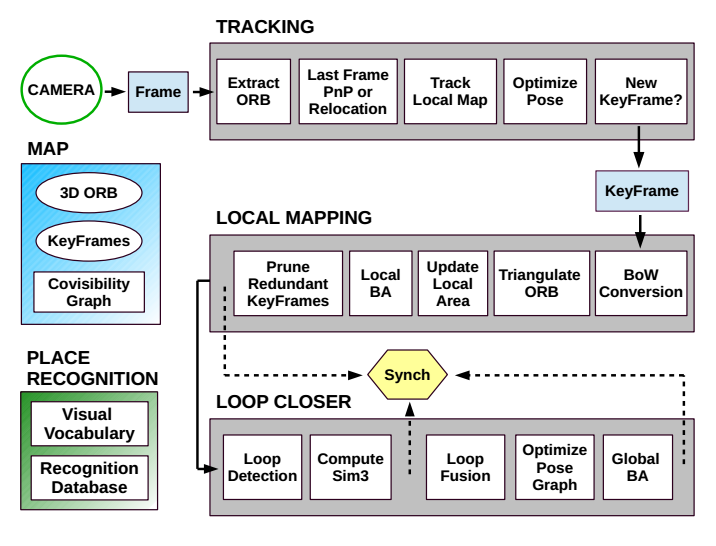
\includegraphics[scale=0.5]{figures/Fig3.6.png}
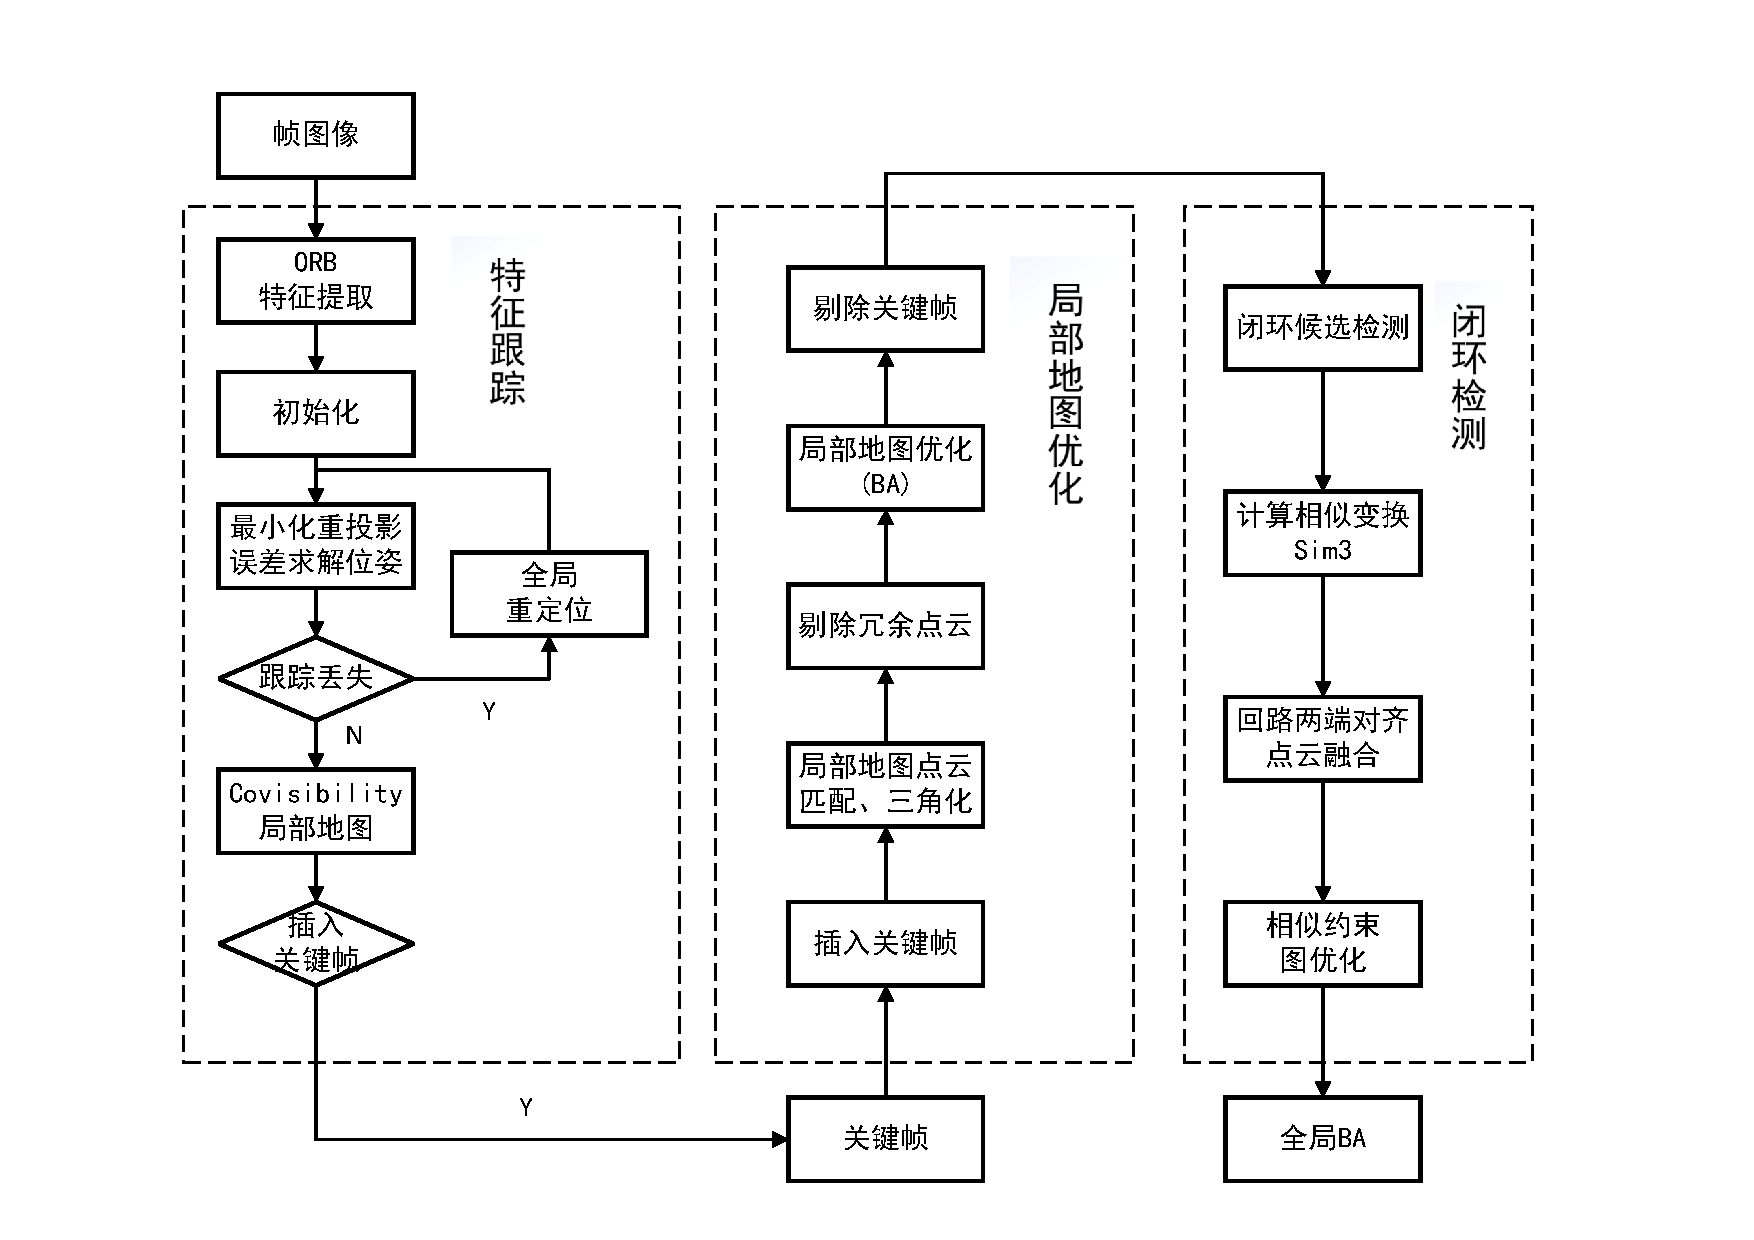
\includegraphics[scale=0.5,angle=-90]{figures/Fig3-6.pdf}
\caption{ORB-SLAM算法流程图}
\label{fig3.6}
\end{figure}

ORB-SLAM主要包括三个模块,特征跟踪,局部地图优化和闭环检测。特征跟踪模块负责提取新图像的特征点,并与临近的关键帧匹配估计当前帧的位姿并选择合适的图像作为新的关键帧;局部地图模块负责维护用于表示局部地图的Covisibility图,求解一个BA问题来优化局部地图中关键帧的位姿并筛选局部地图中的关键帧,剔除冗余;闭环检测模块对全局地图与关键帧进行回环检测,维护一个Pose图约束帧间位姿,消除累计误差。最后在每次闭环检测成功并优化结束后,独立进行一次全局BA,优化地图点位置,提高地图精度和一致性。


\subsubsection*{特征提取与匹配}
图像是由灰度和色彩组成的矩阵,如果直接从矩阵层面考虑运动估计会非常困难,基于特征的SLAM算法从图像中选取一些代表性的特征。为了保证在相机运动之后特征点保持稳定并可以在多个图像中找到,特征点应该满足如下性质
\begin{enumerate}[label={(\arabic*)}]
\item 可重复性:相同特征可以在不同的图像中被找到。
\item 可区别性:不同的特征有不同的表达。
\item 高效性:同一图像中,特征数量远小于像素数量。
\item 本地性:特征仅与小片图像区域相关。
\end{enumerate}

特征点由关键点和描数子两部分组成。关键点指该特征点在图像中的位置,有些特征点具有朝向、大小等信息;描述子通常由方向向量表示,按照人为设计的方式,描述该点周围像素的信息,描述子的设计原则是相似的特征应该有相似的描述子。因而,当两个特征的描述子在向量空间上的距离近似,可以人为是相同的特征。

ORB特征由关键点和描述子两部分组成。其关键点成为"Oriented FAST",FAST是一种图像角点,主要检测局部灰度变化明显的区域,提取速度块。ORB特征对原有的FAST特征点进行改进,添加了尺度和旋转不变性。旋转不变性通过构建尺度金字塔,并在金字塔每层检测角点来实现。旋转不变形则利用灰度质心法,以图像灰度值作为权重计算图像快质心,通过质心和几何中心设计方向向量保证特征旋转不变性;ORB特征的描述子为改进BRIEF描述子,BRIEF是一种二进制描述子,由0,1编码的向量表示关键点周围的两个像素的灰度大小关系。BRIEF使用随机选点的比较,速度快,存储方便,但是不具有旋转不变形。ORB特征在原有BRIEF描述子的基础上利用Oriented FAST关键点的方向信息,获取Steer BRIEF,使ORB特征描述子具有较好的尺度不变形。ORB特征相对于其他特征,如SHIFT、SURF特征,在保证精度和鲁棒性可用的前提下具有更好的计算速度和提取效率,适用于实时性要求较高的视觉SLAM算法。

\subsubsection*{数据关联与运动估计}
在完成图像特征提取后,需要对图像间的相同特征进行匹配。特征匹配是SLAM算法中重要的一部,解决SLAM算法的数据关联,确定了当前图像特征与之前图像特征的对应关系。考虑两个时刻的图像,如果图像$I_t$中提取的特征点$x_t^m,m=1,2,\cdots,M$,在图像$I_{t+1}$中提取到特征点$x_{t+1}^n,n=1,2,\cdots,N$,最简单的方法是进行暴力匹配,对每个特征点$x_t^m$与所有的特征点$x_{t+1}^n$测量描述子之间的距离,取最接近的作为匹配点。描述子距离表示描述子的相似程度,对于浮点类型的描述子可以使用欧氏距离,对于BRIEF这样的二进制描述子,一般使用汉明距——比较描述子不同位的个数。暴力匹配是最直接的方法,单当特征点数量较多,尤其与地图进行匹配时,暴力匹配将消耗很大的计算量,无法满足SLAM算法实时性要求。ORB-SLAM引入恒速模型匹配,假设当前帧的运动与上一帧相同从而得到初始位姿,之后利用出事位姿将上一帧或地图点投影到当前帧就近匹配,极大的提高了匹配速度。

当完成特征点匹配后,需要根据特征匹配关系估计相机运动。首先在初始化阶段,由于单目只知道2D像素坐标信息,需要根据对极几何解决初始位姿估计,对极几何描述了匹配特征点之间的几何关系,如图\ref{fig3.7}所示。

\begin{figure}[h]
\centering
%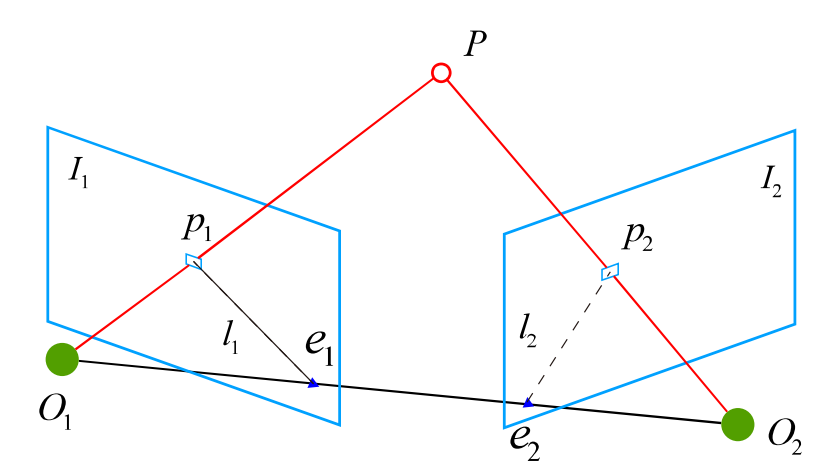
\includegraphics[scale=0.5]{figures/Fig3.7.png}
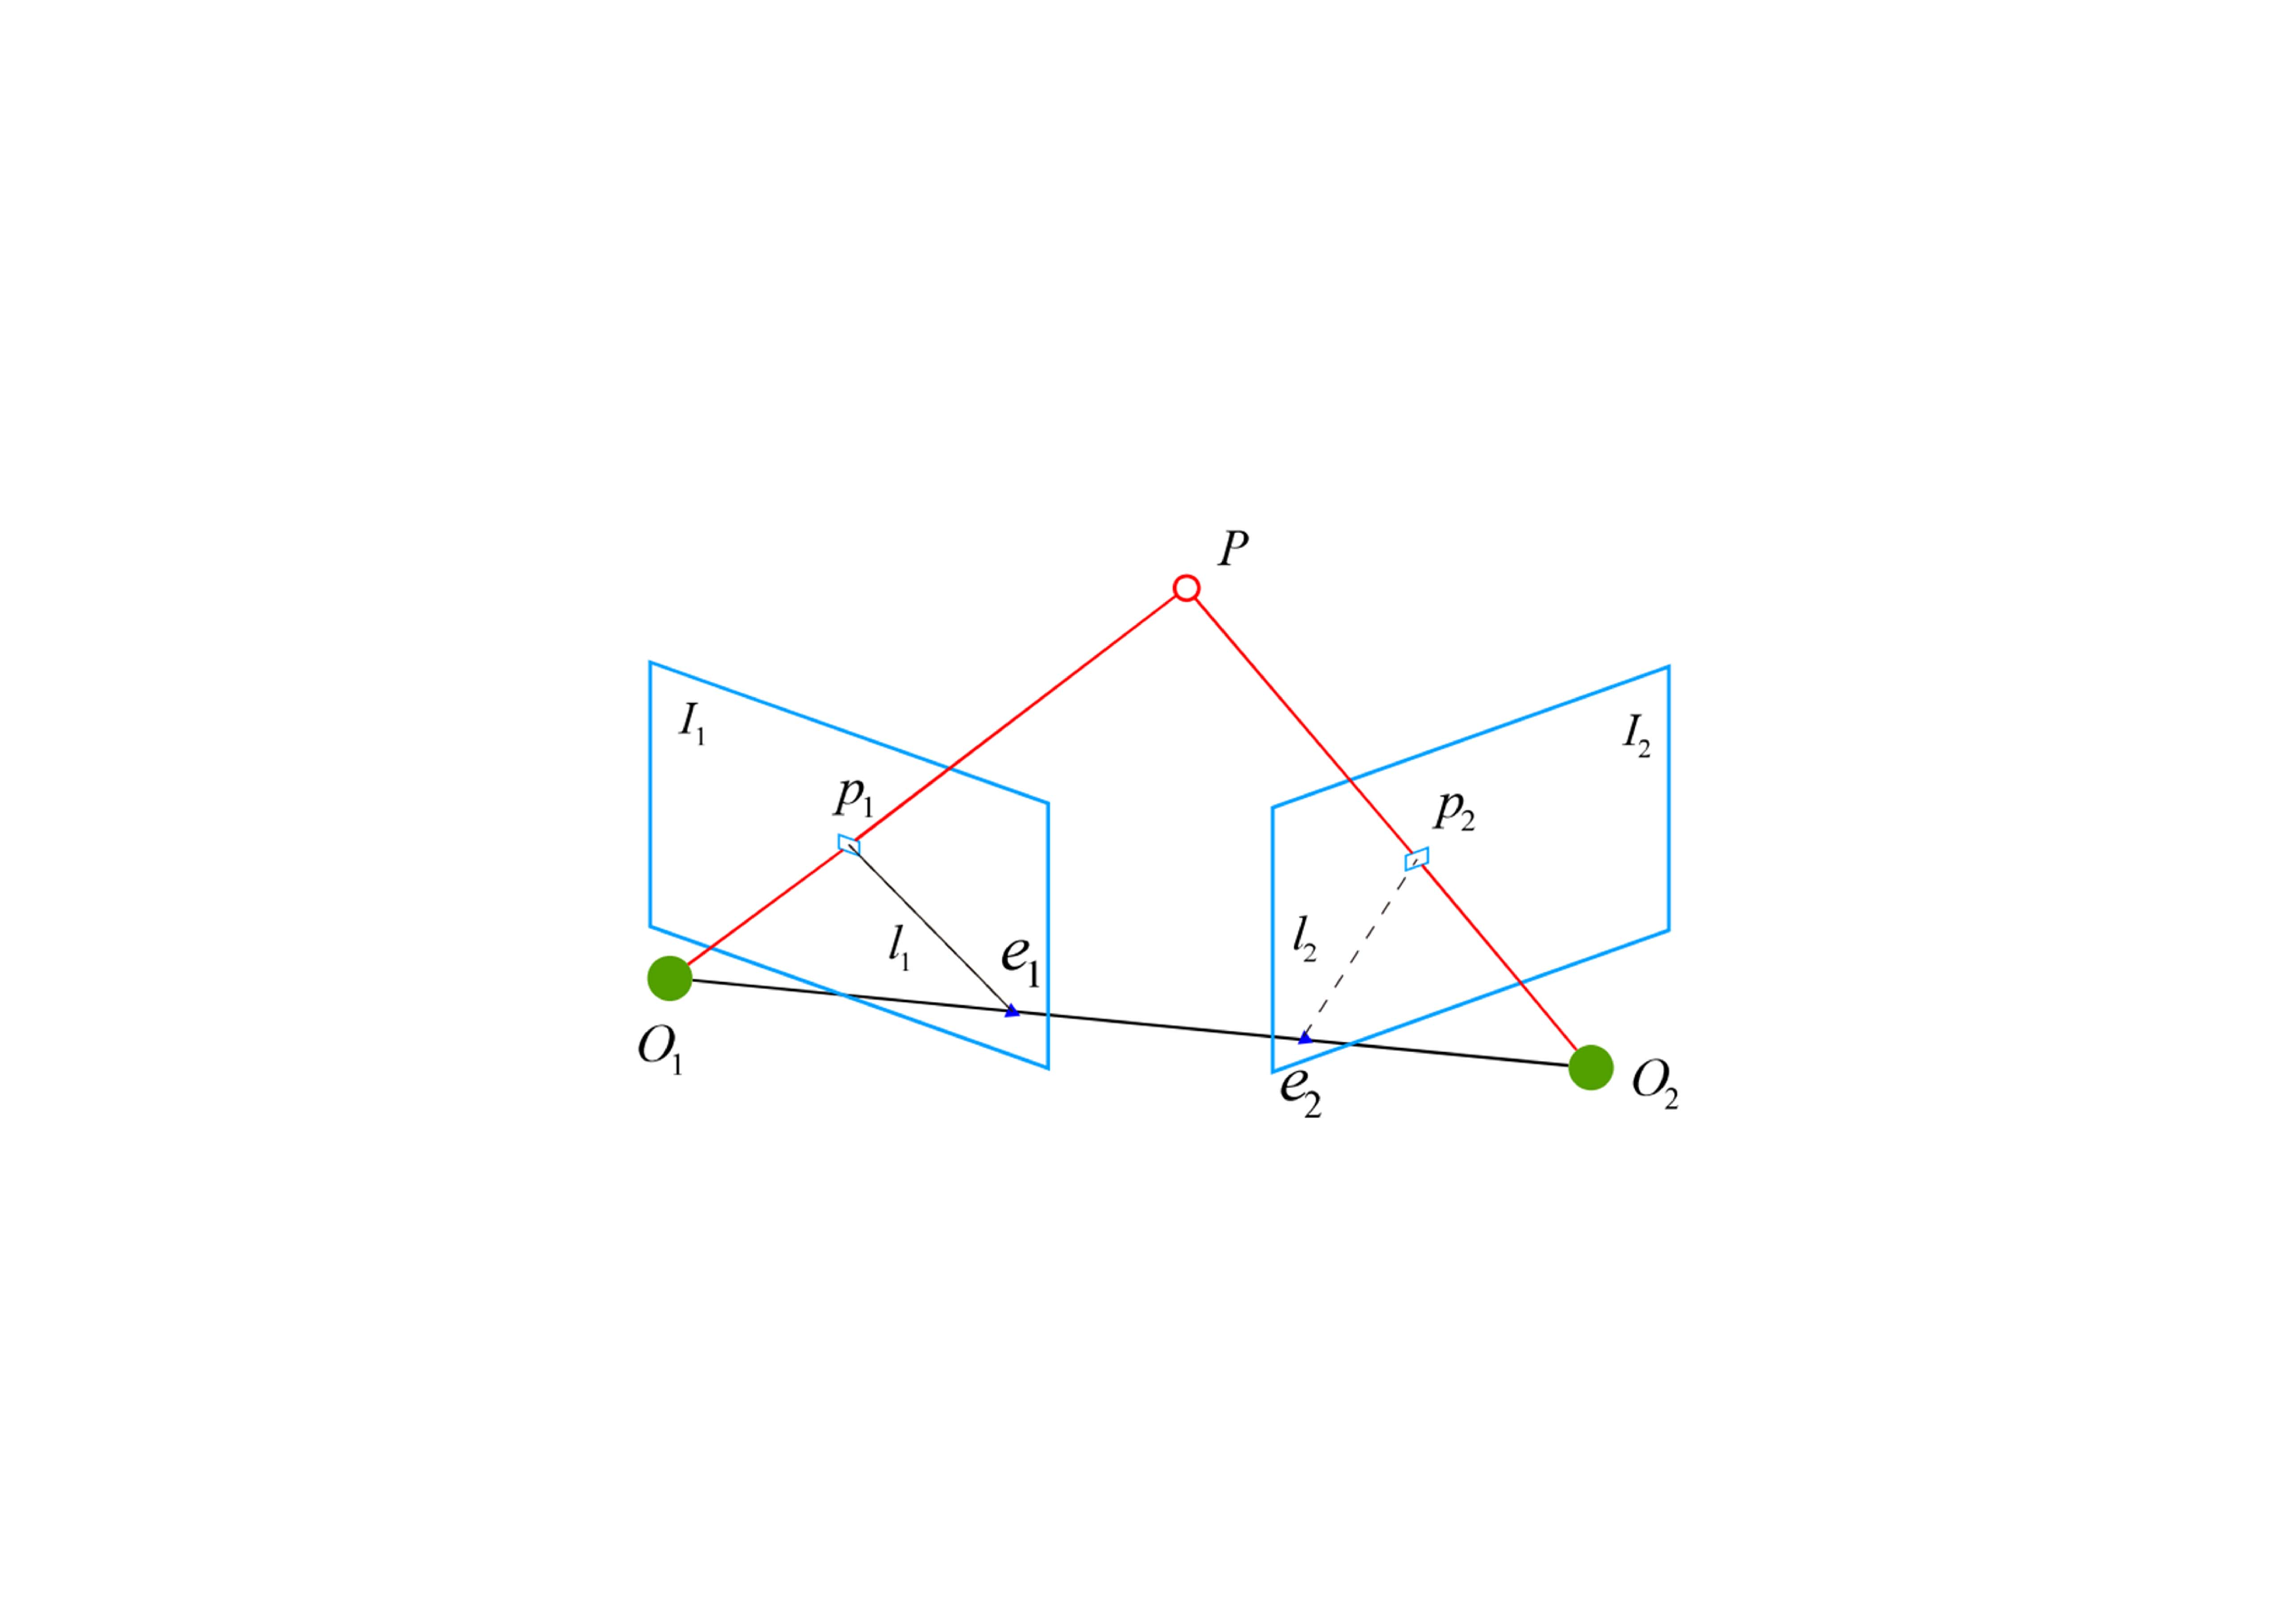
\includegraphics[scale=0.35,angle=-90]{figures/Fig3-7.pdf}
\caption{对极几何约束}
\label{fig3.7}
\end{figure}
假设第一帧到第二帧的相对运动为$\boldsymbol{R}$,$\boldsymbol{t}$,两个相机中心分别为$O_1$,$O_2$。考虑空间点$P=[X,Y,Z]^T$在两帧图像上的对应特征点$\boldsymbol{p}_1$,$\boldsymbol{p}_2$。根据相机投影模型,有
\begin{equation}
\label{equ3.15}
s_1 \boldsymbol{p}_1 = \boldsymbol{K} \boldsymbol{P}, \ \ \ 
s_2 \boldsymbol{p}_2 = \boldsymbol{K} (\boldsymbol{R} \boldsymbol{P}+\boldsymbol{t})
\end{equation}
在公式\eqref{equ3.15}中$\boldsymbol{K}$表示相机内参,$s_1$,$s_2$表示在两相机坐标系下的空间点深度,空间点坐标使用齐次坐标表示,现在取
\begin{equation}
\label{equ3.16}
\boldsymbol{x}_1 = \boldsymbol{K}^{-1} \boldsymbol{p}_1, \ \ \ 
\boldsymbol{x}_2 = \boldsymbol{K}^{-1} \boldsymbol{p}_2
\end{equation}
将方程\eqref{equ3.16}带入方程\eqref{equ3.15}中,可以得到
\begin{equation}
\label{equ3.17}
s_2 \boldsymbol{x}_2 = s_1 \boldsymbol{R} \boldsymbol{x}_1 + \boldsymbol{t}
\end{equation}
将方程\eqref{equ3.17}两侧同左乘$\boldsymbol{t}$的反对称矩阵$\boldsymbol{t}^{\wedge}$,再左乘$\boldsymbol{x}_2^T$,有
\begin{equation}
\label{equ3.18}
\boldsymbol{x}_2^T  \boldsymbol{t}^{\wedge}  \boldsymbol{R} \boldsymbol{x}_1 = \boldsymbol{x}_2^T \boldsymbol{t}^{\wedge} \boldsymbol{x}_2 = 0
\end{equation}
重新带入$\boldsymbol{p}_1$,$\boldsymbol{p}_2$可以得到
$\boldsymbol{x}_2^T$,有
\begin{equation}
\label{equ3.19}
\boldsymbol{p}_2^T \boldsymbol{K}^{-T} \boldsymbol{t}^{\wedge}  \boldsymbol{R} \boldsymbol{K}^{-1} \boldsymbol{p}_1  = 0
\end{equation}
公式\eqref{equ3.18}, \eqref{equ3.19}都称为对极约束,同时包含了旋转和平移信息。两方程中间的矩阵分别记为本质矩阵$\boldsymbol{E} = \boldsymbol{t}^{\wedge}  \boldsymbol{R} $和基本矩阵$\boldsymbol{F} = \boldsymbol{K}^{-T} \boldsymbol{t}^{\wedge}  \boldsymbol{R} \boldsymbol{K}^{-1}$。通过分解以两个矩阵,可以获得两帧图像之间的帧间相对运动。之后对估计运动的两帧关键帧的匹配特征进行三角化,得到出事地图点云的空间坐标。根据之前对极约束中的公式\eqref{equ3.17},同时左乘$\boldsymbol{x}_1^{\wedge}$可以得到
\begin{equation}
\label{equ3.20}
s_2 \boldsymbol{x}_1^{\wedge} \boldsymbol{R} \boldsymbol{x}_2 + \boldsymbol{x}_1^{\wedge} \boldsymbol{t} = s_1 \boldsymbol{x}_1^{\wedge} \boldsymbol{x}_1 = 0
\end{equation}
通过求解方程\eqref{equ3.20}可以直接得到$s_2$,根据求得结果可以很容易得到$s_1$。需要注意的是,由于单目无法提供深度信息,以上估计的位姿和地图点位置无法确定准确的尺度,一般将初始化地图点深度均值归一化为1。

在ORB-SLAM完成初始化得到初始关键帧和地图后,对于之后的帧图像,利用恒速模型提供给每帧图像位姿初值,将上一帧中的地图点投影到当前帧中,在阈值范围内搜索匹配点,通过最小化重投影误差求解当前帧的位姿。考虑$n$个三维空间点P和他们的投影p,当前帧的位姿$\boldsymbol{R}$,$\boldsymbol{t}$用李代数$\boldsymbol{\xi}$表示。假设空间点坐标为$P_i=[X_i,Y_i,Z_i]^T$,其投影的像素坐标为$\boldsymbol{u}_i = [u_i,v_i]T$,根据相机投影模型有
\begin{equation}
\label{equ3.21}
s_i
\begin{bmatrix}
u_i \cr v_i \cr 1\cr 
\end{bmatrix}
=
\boldsymbol{K} \exp\left( \boldsymbol{\xi}^{\wedge} \right)
\begin{bmatrix}
X_i \cr Y_i \cr Z_i \cr 1 \cr
\end{bmatrix}
\end{equation}
方程\eqref{equ3.21}表示根据位姿预测的空间点投影像素位置,由于相机位姿存在误差且系统存在观测误差,观测到的匹配点$p_i$与预测值存在误差,可以构建BA问题优化相机位姿,优化函数为。
\begin{equation}
\label{equ3.22}
\boldsymbol{\xi}^* = \argmin\limits_{\boldsymbol{\xi}} {1 \over 2} \sum\limits_{i=1}^n  \left \Vert \boldsymbol{p}_i - {1 \over s_i} \boldsymbol{K} \exp\left( \boldsymbol{\xi}^{\wedge} \right) \boldsymbol{P}_i  \right \Vert_2^2
\end{equation}
方程\eqref{equ3.22}中的误差称为重投影误差,利用李代数可以构建无约束优化问题,通过高斯-牛顿(G-N)或列文伯格-马夸尔特方法(L-M)等优化方法可以很容易的求解。

%3.3
\section{两种SLAM算法比较}
之前的内容主要针对主流的单目SLAM算法原理进行了分析,本节将在具体数据集上对两个主流的SLAM算法基于直接法的LSD-SLAM和基于特征的ORB-SLAM算法进行实验和比较,对比两种算法的定位精度、鲁棒性和地图重建效果,根据实验结果分析两种SLAM算法的优缺点。结合无人机飞行器的运动特性选择合适的视觉SLAM定位方法,并针对其存在的问题提出改进方案。

\subsubsection*{定位精度}
TUM RGB-D数据集包含了多种室内场景的图像序列,并且每个序列通过外部视觉捕捉系统提供了准确的真实轨迹,适用于评估视觉SLAM系统的定位精度。对单目SLAM算法进行实验测试时,只使用TUM数据集的RGB图像。对于单目SLAM输出的轨迹结果,通过$\mathfrak{sim}(3)$相似变换进行轨迹对齐,比较关键帧的绝对轨迹误差的均方根误差(RMSE),误差表示为:
\begin{equation}
\label{equ3.23}
\begin{aligned}
\boldsymbol{F}_i &\doteq \boldsymbol{Q}_i^{-1} S \boldsymbol{P}_i
\\ 
R\!M\!S\!E(\boldsymbol{F}) &\doteq \left( {1 \over n} \sum\limits_{i=1}^n \left \Vert trans(\boldsymbol{F}_i) \right \Vert^2 \right)^{1 \over 2} 
\end{aligned}
\end{equation}
其中$\boldsymbol{Q}_i$表示真值轨迹第$i$时刻的位置,$\boldsymbol{P}_i$表示估计轨迹第$i$时刻的位置,$\boldsymbol{S}$表示用于对齐估计的$\mathfrak{sim}(3)$相似变换,结果如下表\ref{tab3.1}所示

\begin{table}[h]		%表格环境
% \multicolumn是跨列功能,第一个参数2,表示跨两列,第二个参数c|,表示文字置中,并在栏位右边画一条直线框,最后一个参数即是要填入的文字
%\multirow是跨行功能,第一个参数2,表示跨两行,第二个参数*,表示系统自动调整文字,最后一个参数即是要填入的文字
\newcommand{\tabincell}[2]{\begin{tabular}{@{}#1@{}}#2\end{tabular}}		%单元格内容强制换行
\renewcommand\arraystretch{1.5}		%增加行间距
\centering
\caption{TUM数据集单目SLAM算法轨迹定位精度}   % 表格标题,在表格内容之前
\label{tab3.1}
	\begin{tabular*}{0.9\textwidth}{@{\extracolsep{\fill}}ccc}  %生成行和列的表格
	%\begin{tabular}{p{2cm}p{1.5cm}p{1.5cm}p{1.5cm}}	
	
	\toprule
	
	\multicolumn{1}{c}{\multirow{2}{*}{Seq.}} &
	\multicolumn{2} {c} {\bfseries\tabincell{c} {关键帧轨迹均方根误差 RMSE(cm)}} \\
	\cline{2-3}								%在上一行下面,2-4列画横线
	\multicolumn{1}{c}{}&
	\multicolumn{1}{c}{ORB SLAM}	&
	\multicolumn{1}{c}{LSD SLAM}	\\	
	
	\midrule
	
	\multicolumn{1}{c}{fr1/xyz}		&
	\multicolumn{1}{c}{0.90}		&
	\multicolumn{1}{c}{9.00}		\\
	
	\multicolumn{1}{c}{fr2/xyz}		&
	\multicolumn{1}{c}{0.30}		&
	\multicolumn{1}{c}{2.15}		\\
	
	\multicolumn{1}{c}{fr1/desk}	&
	\multicolumn{1}{c}{1.69}		&
	\multicolumn{1}{c}{10.65}		\\
	
	\multicolumn{1}{c}{fr2/desk}	&
	\multicolumn{1}{c}{0.88}		&
	\multicolumn{1}{c}{4.57}		\\
	
	\multicolumn{1}{c}{fr2/desk\_ person}	&
	\multicolumn{1}{c}{0.63}		&
	\multicolumn{1}{c}{31.73}		\\
	
	\multicolumn{1}{c}{fr3/long\_ office}	&
	\multicolumn{1}{c}{3.45}		&
	\multicolumn{1}{c}{38.53}		\\

	\multicolumn{1}{c}{fr3/sit\_ xyz}	&
	\multicolumn{1}{c}{0.79}		&
	\multicolumn{1}{c}{7.73}		\\	
	
	\multicolumn{1}{c}{fr3/walk\_ halfsph}	&
	\multicolumn{1}{c}{1.74}		&
	\multicolumn{1}{c}{$\boldsymbol{X}$}		\\	
	\bottomrule
	
	\end{tabular*}
\end{table}
表\ref{tab3.1}是在数据集连续测试五次取均值的结果,符号$\boldsymbol{X}$表示运行过程中出现丢失无法完成整个数据集。通过表\ref{tab3.1}可以看出,ORB-SLAM算法的定位精度高于LSD-SLAM,对于存在运动目标的场景具有较好的定位精度。主要原因可能是:(1)基于直接法的LSD-SLAM算法遵从灰度不变假设,对于相机内参和曝光非常敏感,而且直接法SLAM在相机运动过快时无法准确估计位姿;而基于特征的SLAM算法使用特征提取与匹配的方法关联和解算位姿,对传感器参数变化较为鲁棒,并且在快速运动时不易丢失。(2)基于直接法的SLAM算法计算复杂度较大,无法多次优化关键帧位姿并且将关键帧位姿与地图点的联合BA优化简化为pose图优化,影响了定位精度。另外,由于单目无法提供深度信息,因而估计的轨迹缺少尺度信息。

\subsubsection*{地图重建效果}
选择TUM数据集中具有代表性的fr2/xyz,fr2/desk,fr3/long\_ office数据集对比重构效果,重构效果如下图所示
\begin{figure}[h]
\centering
	\subfigure[LSD-SLAM]
    {
		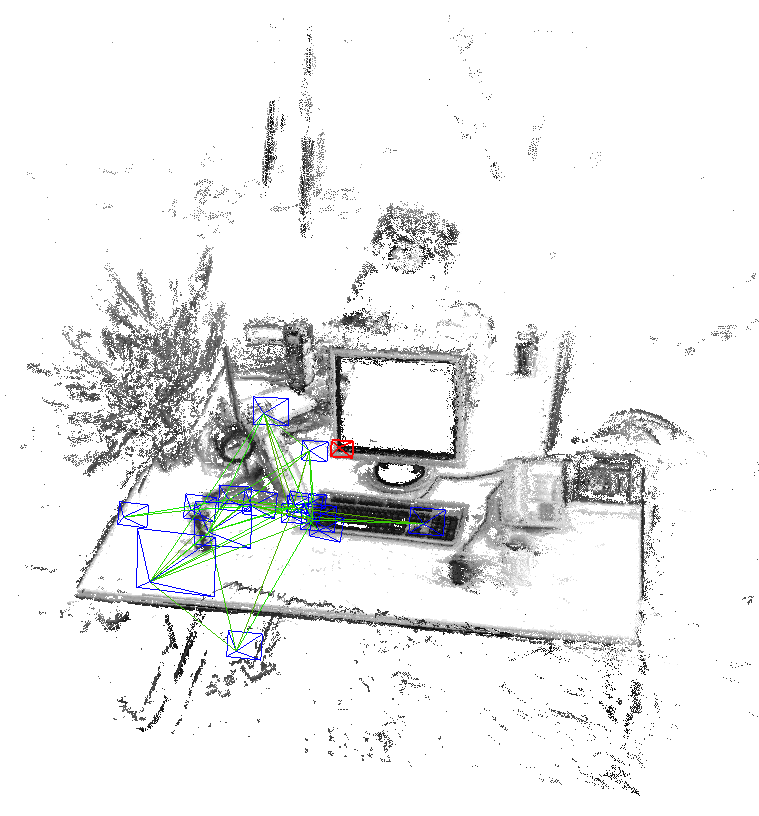
\includegraphics[scale=.24]{figures/Fig3.8_a.png}
	}
	\subfigure[ORB-SLAM]
    {	
		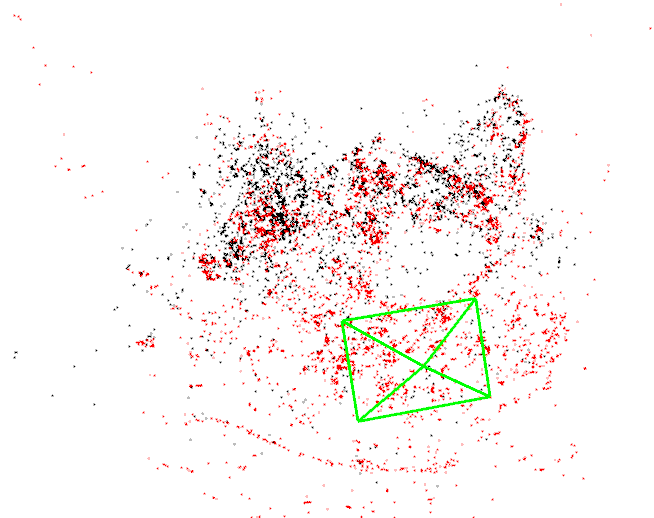
\includegraphics[scale=.3]{figures/Fig3.8_b.png}
	}
\caption{fr2/xyz场景}
\label{fig3.8}
\end{figure}

\begin{figure}[h]
\centering
	\subfigure[LSD-SLAM]
    {
		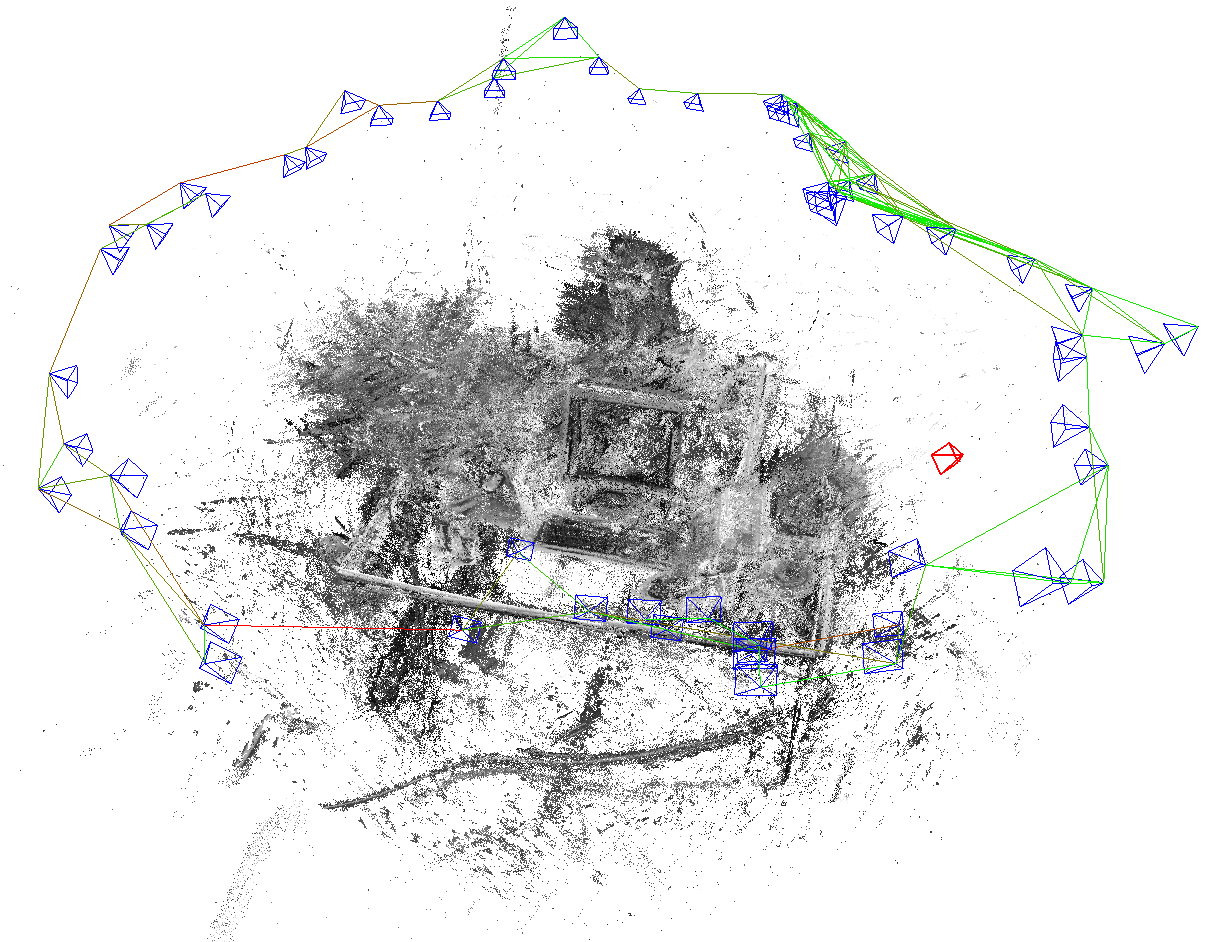
\includegraphics[scale=.15]{figures/Fig3.9_a.png}
	}
	\subfigure[ORB-SLAM]
    {	
		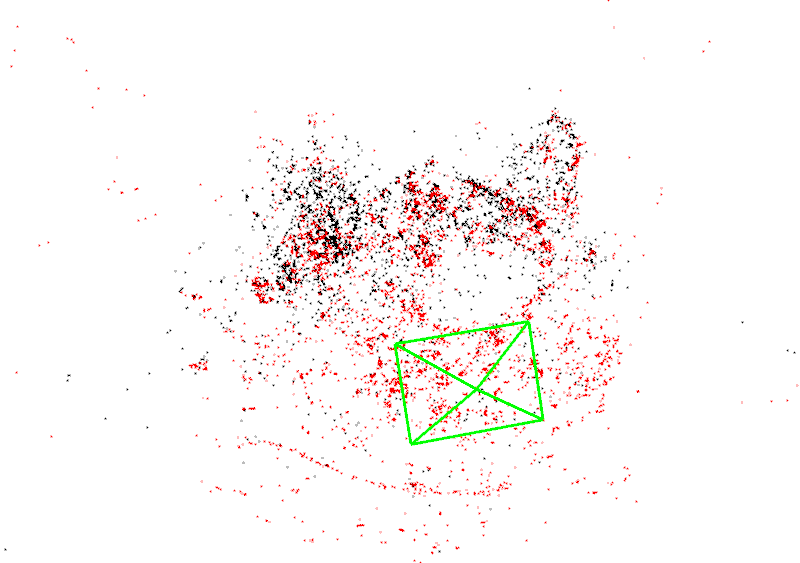
\includegraphics[scale=.3]{figures/Fig3.9_b.png}
	}
\caption{fr2/desk场景}
\label{fig3.9}
\end{figure}

\begin{figure}[h]
\centering
	\subfigure[LSD-SLAM]
    {
		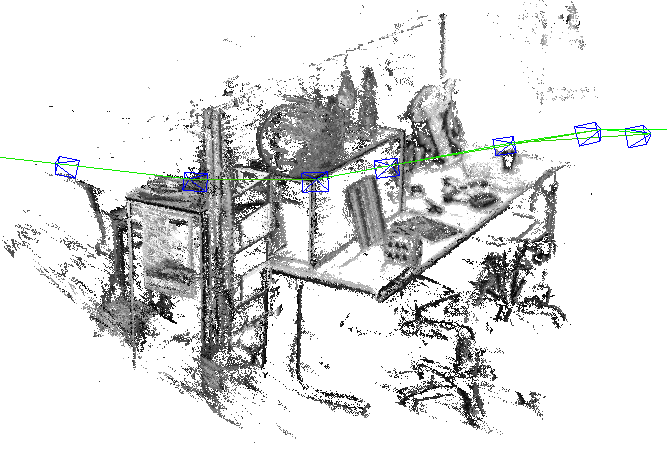
\includegraphics[scale=.25]{figures/Fig3.10_a.png}
	}
	\subfigure[ORB-SLAM]
    {	
		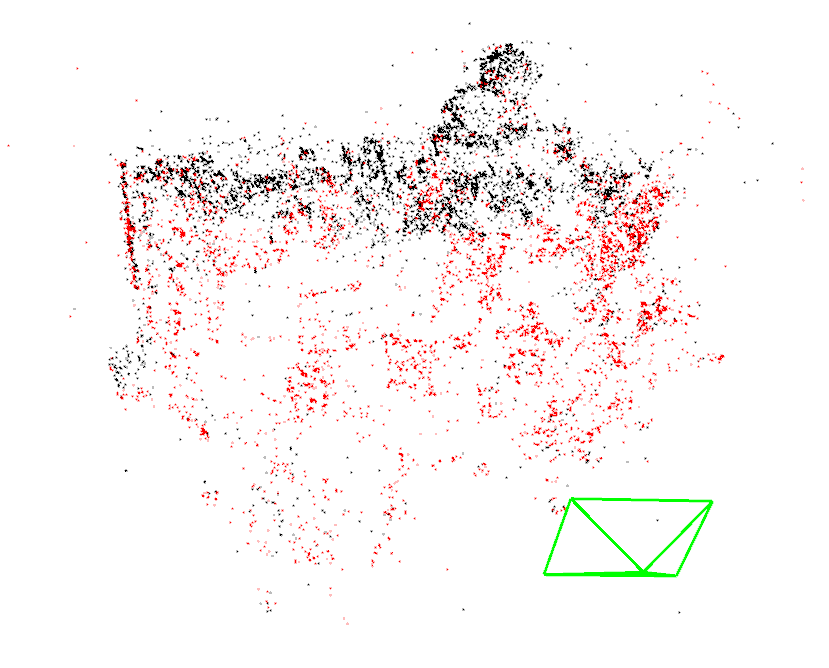
\includegraphics[scale=.21]{figures/Fig3.10_b.png}
	}
\caption{fr3/long\_ office场景}
\label{fig3.10}
\end{figure}

通过对比以上重建结果可以看出,基于直接法的LSD-SLAM算法可以恢复环境的半稠密地图,通过地图可以进行目标识别,导航与任务规划等其他任务;而基于特征的ORB-SLAM算法只能恢复环境稀疏的点云地图,无法提供更多的环境信息。造成这样结果的原因在于,基于特征的SLAM算法只恢复环境的特征点对应的地图点云,考虑特征点的性质:其数量远低于像素数量,因而无法提供丰富的环境场景信息。直接法SLAM关联灰度变化明显区域的像素,而灰度变化明显的像素一般为物体边缘,因而可以恢复出环境的半稠密地图。

%3.4
\section{本章小结}
本章介绍了单目视觉SLAM的结构框架、算法原理和分类,从实现原理,定位精度,鲁棒性和地图重建效果4个方面比较了经典的基于直接法的LSD-SLAM算法和基于特征的ORB-SLAM算法。结果表明,相比于基于直接法的LSD-SLAM算法,基于特征的ORB-SLAM算法具有较好的光度不变性和视角不变性,可以在宽基线条件下稳定匹配,对于快速运动鲁棒性好,适宜作为无人机的感知定位系统。但也存在两个问题,首先基于特征的ORB-SLAM算法重建地图为稀疏点云地图,环境信息较少,无法用于无人机的导航、避障与路径规划;另外,由于单目相机无法提供环境尺度,因而估计得到的轨迹尺度不确定。针对ORB-SLAM算法存在的问题,在第四章研究基于特征的SLAM算法的半稠密重建,提供丰富的环境信息;在第五章研究基于IMU-视觉融合的惯性视觉单目SLAM算法,解决单目SLAM算法的尺度问题。通过以上改进,使得本文研究的单目SLAM算法具有准确的尺度,较好的定位精度和丰富的环境信息,为无人机提供准确的位姿估计和环境信息。




\iffalse
\begin{table}
\newcommand{\tabincell}[2]{\begin{tabular}{@{}#1@{}}#2\end{tabular}}		%单元格内容强制换行
\centering
\caption{TUM数据集下单目SLAM算法定位精度}	% NOTE!  caption goes _before_ the table contents !!
\renewcommand\arraystretch{1.5}		%增加行间距
%\begin{small}							%控制字体大小
\begin{tabular}{p{2cm}p{1.5cm}p{1.5cm}p{1.5cm}}
%\hline									%  结束的那一行画一根水平的直线
\toprule
% \multicolumn是跨列功能,第一个参数2,表示跨1列,第二个参数c|,表示文字置中,并 在栏位右边画一条直线框,最后一个参数即是要填入的文字
\multicolumn{1}{c}{\multirow{3}{*}{Seq.}} & 
\multicolumn{2} {c} {\bfseries\tabincell{c} {Absolute Key Frame Trajectory RMSE(cm)}} \\
\cline{2-3}								%在上一行下面,2-4列画横线
\multicolumn{1}{c}{}&   
\multicolumn{1}{c}{\bfseries \tabincell{c}{LSD-SLAM} } &     
\multicolumn{1}{c}{\bfseries \tabincell{c}{ semi-dense \\mono-VO}}  \\
%\multicolumn{1}{c}{\bfseries \tabincell{c}{ RGB-D \\SLAM}} \\	
%\cline{1-3}
\midrule
\multicolumn{1}{c}{fr2/desk}	&
\multicolumn{1}{c}{5.65}		&
\multicolumn{1}{c}{13.50}      \\
%\multicolumn{1}{c}{2.58}   \\

\multicolumn{1}{c}{Fr2/xyz}  &
\multicolumn{1}{c}{2.15}     &
\multicolumn{1}{c}{3.79}      \\
%\multicolumn{1}{c}{1.34}    \\

\multicolumn{1}{c}{sim/slowmo}  &
\multicolumn{1}{c}{0.37}        &
\multicolumn{1}{c}{2.21}        \\
%\multicolumn{1}{c}{0.13}        \\
%\hline
\bottomrule
\end{tabular}
%\end{small}	
\end{table}
\fi




\iffalse
The current frames will replace the current key frames according with the Direct SE(3) image alignment. An existing key frame ${k_i} = ({I_i},{D_i},{V_i})$, the relative posture ${\xi _{ji}} \in se(3)$ of a new image ${I_j}$ is obtained by minimizing the variance-normalized photometric error

\begin{equation}
E_{p}(\xi _{ji}) = \sum\limits_{p \in \Omega _{D_{i}}} \left\|  \frac{r_{p}^{2} (p,\xi_{ji})}{\sigma_{r_{p}}^{2} (p,\xi_{ji})}  \right\|_{\delta}
\end{equation}


\begin{equation}
r_{p}(p,\xi _{ji}): = I_{i}(p) - I_{j}(\omega (p,D_{i}(p),\xi _{ji}))
\end{equation}

\begin{equation}
\sigma _{r_{p}} ^{2}(p,\xi _{ji}): = 2\sigma _{I} ^{2} + {\left( \frac {\partial r_{p}(p,\xi_{ji})} {\partial D_{i} (p)} \right)^{2}} V_{i}(p)
\end{equation}

The formula (13) is the Huber norm and applied to the normalized residual.

\begin{equation}
{\left\| r^{2} \right\|_{\delta}}:=\left\{\begin{array}{ll}
\frac {r^{2}} {2\delta}            & |r|\leq \delta       \\
|r|-\frac {\delta} {2}      & |r| > \delta
\end{array} \right.
\end{equation}




If the camera moves too far away from the existing map, a new key frame is created from the most recent tracked image. We threshold a weighted combination of relative distance and angle to the current key frame

\begin{equation}
dist({\xi _{ji}}): = \xi _{ji}^TW{\xi _{ji}}
\end{equation}

Where W is a diagonal matrix containing the weights. Note that, as described in the following section, each key frame is scaled such that its mean inverse depth is one. This threshold is therefore relative to the current scale of the scene, and ensures sufficient possibilities for small-baseline stereo comparisons.

Once a new frame is chosen to become a key frame, its depth map is initialized by projecting points from the previous key frame into it, followed by one iteration of spatial regularization and outlier removal [5]. Afterwards, the depth map is scaled to have a mean inverse depth of one -this scaling factor is directly incorporated into the sim(3) camera pose. Finally, it replaces the previous key frame and is used for tracking subsequent new frames.

In contrast to RGB-D or Stereo SLAM, monocular SLAM is inherently scale-ambivalent, the absolute scale of the world is not observable. Over long trajectories this leads to scale-drift, which is one of the major sources of error [9]. Further, all distances are only defined up to scale, which causes threshold-based outlier rejection or parametrized robust kernels to be ill-defined.

We select an advanced method in [1] for better perform direct, scale-drift image alignment, which is used to align two differently scaled key frames. For the photometric residual ${r_p}$, the depth residual ${r_d}$ which penalizes deviations in inverse depth between key frames, allowing to directly estimate the scaled transformation between them. The total error function becomes

\begin{equation}
E({\xi _{ji}}): = {\sum\limits_{p \in {\Omega _{{D_i}}}} {\left\| {\frac{{r_p^2(p,{\xi _{ji}})}}{{\sigma _{{r_p}(p,{\xi _{ji}})}^2}} + \frac{{r_d^2(p,{\xi _{ji}})}}{{\sigma _{{r_d}(p,{\xi _{ji}})}^2}}} \right\|} _\delta }
\end{equation}
the depth residual is computed

\begin{equation}
r_{d}(p,\xi _{ji}): = [p^{'}]_{3} - D_{j}([p^{'}]_{1,2})
\end{equation}

% 公式换行用 \\ 
\begin{equation}
\begin{split}
\sigma_{r_{d}(p,\xi_{ji})} ^{2} :=V_{j}( [ p^{'} ]_{1,2} )  {\left( \frac {\partial r_{d}(p,\xi_{ji})} {\partial D_{j} \left[ p^{'} \right]_{1,2}}  \right)^{2}} + V_{i}(p) \left( \frac {\partial r_{d}(p,\xi_{ji})} {\partial D_{j}(p)} \right)
\end{split}
\end{equation}

After a new key frame ${k_i}$ is added to the map, a number of possible loop closure key frames ${k_{ji}},....{k_{jn}}$ is collected. We use the closet ten key frames, as well as a suitable candidate. To avoid insertion of false or falsely tracked loop closures, we then perform a reciprocal tracking check. For each candidate ${k_{jk}}$ we independently track ${\xi _{{j_k}i}}$ and ${\xi _{i{j_k}}}$.

\begin{equation}
e\!(\!{\xi _{{j_k}i}},{\xi _{i{j_k}}})\!: \!= \!{\!(\!{\xi _{{j_k}i}} \!\circ \!{\xi _{i{j_k}}})\!^T}{\!(\!{\Sigma _{{j_k}i}}\! +\! Ad{j_{{j_k}i}}{\Sigma _{i{j_k}}}Adj_{{j_k}i}^T\!)\!^{ - 1}}\!(\!{\xi _{{j_k}i}}\! \circ\! {\xi _{i{j_k}}}\!)
\end{equation}

Only if the two estimates are statistically similar, if formula (18) is sufficiently small, they are added to the global map. For this, the adjoint $Ad{j_{{j_k}i}}$ is used to transform ${\Sigma _{i{j_k}}}$ into the correct tangent space.

The map is represented as a pose graph of keyframes: Each keyframe $\kappa_{i}$ consists of a camera image $I_{i}\!:\!\Omega_{D_{i}}\!\rightarrow \!{\mathbb{R}}$,an inverse depth map $D_{i}\!:\!\Omega_{D_{i}}\!\rightarrow \!{\mathbb{R}}^{+}$, and the variance of the inverse depth $ V_{i}\!:\!\Omega_{D_{i}}\!\rightarrow \!{\mathbb{R}}^{+}$.Note that the depth map and variance are only defined for a subset of pixels $ \Omega_{D_{i}}\!\subset\!\Omega_{i} $, containing all image regions in the vicinity of sufficiently large intensity gradient, hence semi-dense.Edges $ \varepsilon_{ji}$ between keyframes contain their relative alignment as similarity transform $ \xi_{ji}\in sim(3) $, as well as the corresponding covariance matrix $\Sigma_{ji} $

The map, consisting of a set of keyframes and tracked sim(3)-constraints, is continuously optimized in the background using pose graph optimization. The
error function that is minimized is in accordance with the left-multiplication convention
\begin{equation}
E(\xi\!_{W\!_{1}}\!...\!\xi\!_{W\!_{n}})\!:\!= \sum\limits_{(\!\xi\!_{ji},\Sigma\!_{ji}\!)\!\in\!\varepsilon}\!(\!\xi_{ji}\!\circ\!\xi_{\!W_{i}\!}^{-1}\! \!\circ\!\xi_{\!W\!_{j}}\!)\!^{T}\!\Sigma_{\!j\!i}^{\!-1\!}\!(\!\xi_{ji}\!\circ\!\xi_{\!W_{i}\!}^{-1}\! \!\circ\!\xi_{\!W\!_{j}}\!)
\end{equation}
\fi

%%==================================================
%% chapter04.tex for BIT Master Thesis
%% modified by yang yating
%% version: 0.1
%% last update: Dec 25th, 2016

%% modified by Meng Chao
%% version: 0.2
%% last update: May 29th, 2017
%%==================================================
\chapter{基于特征的单目半稠密SLAM算法}
\label{chap:Semi-Dense}

针对第三章提到的基于特征的单目SLAM算法构建地图稀疏,无法用于导航和后续任务规划的问题,本章研究一种改进的基于特征的单目SLAM算法,在原有基于特征的ORB-SLAM算法的基础上,参考直接法SLAM半稠密地图构建的原理,构建环境的半稠密地图。不同于直接法SLAM中使用多帧连续帧对参考帧逆深度进行滤波的方法,本文使用经过局部BA(local BA)和位姿图(pose graph)优化后的关键帧进行重构,可获得较高精度的定位和地图重构效果。改进的基于特征的单目SLAM算法主要包括5个部分,立体搜索约束,极线搜索和块匹配,逆深度假设融合,帧内逆深度假设一致性检验和帧间逆深度假设一致性检验,其算法流程图如图\ref{fig1}所示,具体算法流程如下:
\begin{enumerate}[label={(\arabic*)}]

\item 对选取的关键帧$K_i$,提取图像中像素灰度梯度满足阈值的像素点,在临近的$N$个关键帧中进行极线搜索,得到像素的逆深度假设。

\item 考虑到图像在观测过程中存在噪声、视差过小和二义性等问题,假设逆深度服从高斯分布,并且认为相机关键帧的位姿是准确的,不考虑位姿的不确定性。

\item 由于关键帧之间的极线搜索是在宽基线条件下进行,搜索范围较大,需要考虑匹配过程中的误匹配。除考虑更多像素匹配约束外,采用高斯分布表示逆深度图中像素$p$的逆深度假设$N(\rho_p, \sigma_{\rho_p}^2)$,通过融合一致的逆深度假设降低误匹配的影响。

\item 对关键帧逆深度图中的像素逆深度进行融合,并且通过帧内逆深度假设一致性检验剔除与临近像素逆深度不一致的像素。

\item 完成当前关键帧和其相邻关键帧的逆深度假设计算后,对其当前帧和相邻帧的像素逆深度进行一致性检验,剔除不一致的像素逆深度,并通过最小化深度误差函数优化像素深度。

\end{enumerate}

本文改进的基于特征的单目SLAM算法是在宽基线条件下进行的关键帧间极线搜索,宽基线的极线搜索容易导致误匹配和离群值影响重构效果。因而相比于基于直接法的半稠密SLAM算法,为了提高本算法的鲁棒性,进行极线搜索时除考虑灰度梯度大小和方向的匹配性外,还应进行逆深度假设融合和帧内与帧间逆深度假设一致性检验,剔除宽基线极线搜索的误匹配点,从而提升重构效果。

%4.1 半稠密ORB SLAM重构流程
\begin{figure}
\label{fig1}

\end{figure}





% 4.1
\section{立体搜索约束}
本章改进的基于特征的单目SLAM算法可以提供相机位姿$R,t$, 用于像素对应匹配点的搜索进而得到像素逆深度假设。由于已知当前关键帧ORB特征点的深度信息,可以估计当前关键帧的最大逆深度$\rho_max$, 最小逆深度$\rho_min$和像素逆深度的先验信息$N\left( \rho_0,\sigma_{\rho_0}^2  \right)$,其中$\rho_{max}=\rho_0+2\sigma_{\rho_0}$,$\rho_{min}=\rho_0-2\sigma_{\rho_0}$。另外,通过Covisibility图可以获得与当前关键帧$K_i$具有最多共视关系的前$N$个关键帧的集合$K$,从而完成关键帧间的立体搜索。通过立体搜索约束求解当前关键帧的逆深度假设时,应在关键帧插入之后一个帧率的时间内不处理新插入关键帧。一方面可以避免由于局部BA导致的共视图结构变化;另一方面可以引入当前关键帧之后的关键帧,提高重建效果。


%4.2
\section{极线搜索与块匹配}
对于当前关键帧$K_i$中像素梯度的模大于$\lambda_G$的像素$p$,会在关键帧$K_j \in K$的极线$l_j$上$\left[ \rho_{min}, \rho_{max} \right]$范围内进行搜索,寻找匹配的像素点,如图\ref{fig4.1}所示。极线利用基本矩阵$F_{ji}$求得,极线搜索方程如下所示。
\begin{equation}
\label{equ4.1}
x_j^T F_{ji}x_p = x^T_jl_j=0 \rightarrow v_j = m \cdot u_j+n
\end{equation}

\begin{figure}
\label{fig4.1}

\end{figure}

不同于直接法SLAM中的窄极线匹配,本章的改进算法极线搜索是在宽基线条件下进行的,因而除了区块匹配外,需要加入更多约束。除了比较像素灰度$I$之外,还需要比较像素的梯度模$G$和梯度方向$\Uptheta$,从而在极线$l_j$上找到合适的像素匹配。根据以下设计约束, 排除$l_j$极线上不满足条件的像素。


\begin{enumerate}[label={(\arabic*)}]

\item 属于关键帧$K_j \in K$上的像素$p_j$必须在图像中像素梯度大的区域,像素梯度应大于阈值,$G(u_j)> \lambda_G$。

\item 考虑到匹配的二义性与沿极线方向的像素梯度有关,因而像素梯度方向不能与极线方向垂直,满足$\vert \Uptheta(u_j)-\Uptheta_L \pm \pi \vert < \lambda_L$,其中$\Uptheta_L$表示基线方向。

\item 图像的匹配像素$p_j$与$p_i$的梯度方向应该相近,满足$\vert \Uptheta(u_j)-(\Uptheta_L \pm \Delta \theta_{j,i} \vert < \lambda_\theta $,其中$\Delta \theta_{j,i}$表示两帧图像之间的旋转角度。

\end{enumerate}
以上区块匹配约束可以剔除关键帧$K_j \in K$极线上$l_j$的大部分像素点,剩余的为关键帧$K_i$中的像素$p$可能的匹配点。为了比较两个像素点的相似性, 定义像素相似误差函数$e(u_j)$:
\begin{equation}
\label{equ4.2}
\begin{aligned}
& e(u_j) = {r_I^2 \over \sigma_I^2} + {r_G^2 \over \sigma_G^2} \\ 
& r_I = I_p-I(u_j),\  r_G = G_p-G(u_j)
\end{aligned}
\end{equation}
其中$r_I$和$r_G$表示像素灰度和梯度误差,$\sigma_I$和$\sigma_G$表示像素灰度和梯度的标准差。由于像素梯度是根据像素的灰度计算得到,若利用施密特算子$\triangledown$计算梯度, 则像素灰度与梯度的误差具有相性,
$\sigma_G^2=\theta \sigma_I^2$ , $ \theta = 0.23$。公式\ref{equ4.2}可以简化为
\begin{equation}
\label{equ4.3}
 e(u_j) = \left( {r_I^2}+{1 \over \theta} r_G^2 \right) {1 \over \sigma_I^2}
\end{equation} 

相似误差函数最小化的坐标$u_0$表示的像素为对应的匹配像素, 其灰度误差和梯度误差为$r_{I_0}$,$r_{G_0}$,误差函数导数为
\begin{equation}
\label{equ4.4}
{\partial e \over \partial u_j } = -{ -2(r_I g+ { 1 \over \theta} r_G q )  \over \sigma_I^2 }
\end{equation}
令其中$g$是灰度梯度的模,$q$是灰度梯度导数的模,方向与极线相同。
\begin{equation}
\label{equ4.5}
\begin{aligned}
& g \approx { {I(u_j+1) - I(u_j-1)} \over 2 } \\
& q \approx { {G(u_j+1) - G(u_j-1)} \over 2 } 
\end{aligned}
\end{equation}

令公式\ref{equ4.4}等于$0$可以得到匹配的像素坐标$u_0$,实际情况下像素坐标$u_0$是沿极线以像素为步长搜索得到的整数坐标,而公式\ref{equ4.4}的解不一定是整数。设真值为$u_0^*=u_0+\Delta u$,对方程\ref{equ4.2}中的误差进行一阶泰勒近似,带入导数等于$0$的公式\ref{equ4.4}中可以得到
\begin{equation}
\label{equ4.6}
\Delta u = {{ r_I(u_0) g(u_0)+ {1 \over \theta} r_G(u_0)q(u_0) } \over {g^2(u_0)+ { 1 \over \theta} q^2(u_0)}}
\end{equation}
匹配像素的亚像素精度坐标为
\begin{equation}
\label{equ4.7}
u_0^* = u_0 + {{ r_I(u_0) g(u_0)+ {1 \over \theta} r_G(u_0)q(u_0) } \over {g^2(u_0)+ { 1 \over \theta} q^2(u_0)}}
\end{equation}

根据误差传递理论,通过像素灰度的方差$\sigma_I^2$可以得到匹配像素坐标$u_0^*$的不确定性。
\begin{equation}
\label{equ4.8}
\sigma_{u_0^*}^2 = \left \vert { \partial u^* \over \partial r_I(u_0) }  \right \vert \sigma_I^2 + \left \vert { \partial u^* \over \partial r_G(u_0) }  \right \vert \sigma_G^2 = { \sigma_I^2 \over g^2(u_0) + {1 \over \theta} q^2(u_0) }
\end{equation}
根据像素坐标不确定性可以知道,沿极线方向像素灰度梯度和像素灰度梯度导数的模越大,匹配的可靠性越高。

为了得到匹配像素的逆深度假设不确定性,需要计算当前关键帧$K_i$中像素$p$的逆深度$\rho_p$。根据地图点云的三角化公式$s_jX_j = s_pR_{ji}X_p+t_{ji}, \  X_j = K^{-1}P_j, X_p = K^{-1}P_p$,可以得到像素逆深度为
\begin{equation}
\label{equ4.9}
\rho_p(u_j) = { r_z^{ji} X_p (u_j-c_x) - f_x r_x^{ji} X_p  \over - t_z^{ji}(u_j-c_x)+f_x t_x^{ji} }
\end{equation}
其中$r_x^{ji}$,$r_z^{ji}$表示两帧间的旋转矩阵$R_{ji}$的第一行和第三行,$t_x^{ji}$,$t_z^{ji}$表示来两帧间的平移向量$t_{ji}$的第一个和第三个元素;$f_x$,$c_x$是相机内参;$\rho_p = { 1 \over s_p}$,$P_j= \left [ u_j, v_j, 1 \right ] ^T$,利用方程\ref{equ4.9}可以得到像素$p_i$与像素$p_j$对应的逆深度假设$N(\rho_j, \sigma_{\rho_j}^2)$。
\begin{equation}
\label{equ4.10}
\begin{aligned}
& \rho_j = \rho_p(u_0^*) \\ 
& \sigma_{\rho_j} = max \left( \left \vert  \rho_p(u_0^*+\sigma_{u_0^*})-\rho_j \right \vert , \  \left \vert  \rho_p(u_0^*-\sigma_{u_0^*})-\rho_j \right \vert \right)
\end{aligned}
\end{equation}

在以上的逆深度假设推导过程中,并没有像直接法SLAM一样引入帧间小旋转运动假设,因而本算法的逆深度假设不确定性具有一般性。


%4.3
\section{逆深度假设融合}
根据之前4.2节中介绍的方法,每个像素可以得到一组逆深度假设。由于存在极线上的像素逆深度立体搜索约束,且极线上匹配的像素需满足之前提到的像素梯度约束,因而逆深度假设的个数可能不足$N$个。另外,由于像素的相似性和遮挡,以上逆深度假设中存在离群值。为了验证像素逆深度假设,在像素对应的一组逆深度假设中至少应该找到$\lambda_N$个一致假设。利用$\chi^2$假设检验(置信区间$95\%$,自由度2),验证两个逆深度假设分布的一致性。
\begin{equation}
\label{equ4.11}
{ (\rho_a - \rho_b)^2 \over \sigma_a^2 }+{ (\rho_b - \rho_a)^2 \over \sigma_b^2} < 5.991
\end{equation}

每次从一组像素的逆深度假设中选取一个,与其他逆深度假设进行一致性检验,若与其一致的逆深度假设数量超过$\lambda_N$个,则对该组逆深度按照公式\ref{equ4.12}进行融合,像素$p$融合后的逆深度假设服从$N(\rho_p,\sigma_{\rho_p}^2)$,其中$n$表示通过检验的逆深度假设数量。
\begin{equation}
\label{equ4.12}
\rho_p = { {\sum\limits_n {1 \over \sigma_{\rho_j}^2} \rho_j } \over \sum\limits_n {1 \over \sigma_{\rho_j}^2}  }, \ 
\sigma_{\rho_p}^2 = {1 \over  \sum\limits_n { 1 \over \sigma_{\rho_j}^2}  }
\end{equation}


%4.4
\section{帧内逆深度假设一致性检验}
在完成当前关键帧$K_i$中像素的逆深度假设计算和融合后,需要对帧内所有逆深度假设进行一致性检验,用于剔除像素逆深度假设中的离群值。首先,通过公式\ref{equ4.11}检验某像素和它临近的8个像素点的逆深度假设的一致性,若一致的逆深度假设数量大于2,则保留该像素点的逆深度假设,否则剔除该点逆深度假设。若保留该像素,其逆深度根据公式\ref{equ4.12}进行融合,不确定性为所有参与逆深度假设检验的像素中的最小不确定性。对于处于像素灰度变化明显区域但没有逆深度假设的像素点,若在该像素周围至少有两个逆深度假设一致的像素,则给该像素点添加逆深度假设,逆深度为附近一致逆深度假设的逆深度均值,不确定性是附近一致逆深度假设中的最小值,该方法可以增加地图重建的稠密性,起到平滑地图的作用。

%4.5
\section{帧间逆深度假设一致性检验}
在当前关键帧$K_i$的$N$个临近关键帧的逆深度地图全部计算完成后,对关键帧$K_i$中像素的逆深度假设进行帧间一致性检验。对于关键帧$K_i$中的像素$p$对应的逆深度$\rho_p$,将其投影到$K_i$临近的关键帧$K_j \in K$中,并计算像素$p$在关键帧$K_j \in K$中对应点的逆深度:
\begin{equation}
\label{equ4.13}
\begin{aligned}
& x_j = K R_{ji} {1 \over \rho_p} X_p + Kt_{ji} \\ 
& \rho_j = { \rho_p \over r_z^{ji}X_p+\rho_p t_z^{ji} }
\end{aligned}
\end{equation}
其中$x_{j}$表示关键帧$K_i$中的像素$p$在$K_j \in K$中对应点的像素坐标。若$x_j$不是证书像素坐标,搜索$x_{j}$临近的4个像素,通过$\chi^2$假设检验(置信区间$95\%$,自由度$1$),检验是否与$x_j$逆深度假设一致。
\begin{equation}
\label{equ4.14}
{ (\rho_j - \rho_{j,n})^2 \over \sigma_{\rho_{j,n}}^2 } < 3.84
\end{equation}

如果在$\rho_{j,n}$中存在与$x_j$逆深度假设一致的像素点,则可以保留像素点$x_j$的逆深度假设。如果在当前关键帧$K_i$的$N$个临近关键帧中至少有$\lambda_N$个关键帧可以找到像素p的对应像素点$x_j$的逆深度假设,则保留当前关键帧$K_i$中像素$p$的逆深度假设。

最后对关键帧像素进行重投影,以深度$d_p = { 1 \over \rho_p }$为优化变量,利用公式\ref{equ4.15}通过高斯-牛顿方法最小化深度误差函数,优化像素点的逆深度,提高重构精度。
\begin{equation}
\label{equ4.15}
d_p^* = \min_{d_p} \sum\limits_{j,n} \left( d_{j,n} - d_p r_z^{ji} X_p - t_z^{ji}  \right)^2  {1 \over {d_{j,n}^4 \sigma_{\rho_{j,n}}^2 }}
\end{equation}
优化的目标函数选择深度作为优化变量而不是逆深度,是因为从方程\ref{equ4.13}中可以发现,以深度作为变量时,深度误差函数是线性的。并考虑深度对应的不确定,不同深度置信度在总误差的权重不同,优化更为精确。




\section{本章小结}

采取了什么方法,针对出现的问题进行优化,表现出了比现有算法更好的性能。







\iffalse
We evaluate the LSD algorithm hand holding camera in indoor environment. We test two time for the different sample key frames. The result is show in Fig.4 The picture (a) and (b) are the reference image and the key frame. The (c) and (d) are the reconstruction 3D map of the LSD-SLAM. The result is expressed the more key frames can be get the more detail of the environment, now that the noisy of the environment will affect the performance of LSD.

\begin{figure}
    \centering
       %\begin{minipage}{5cm}
       	  \subfigure[]
       	  {
          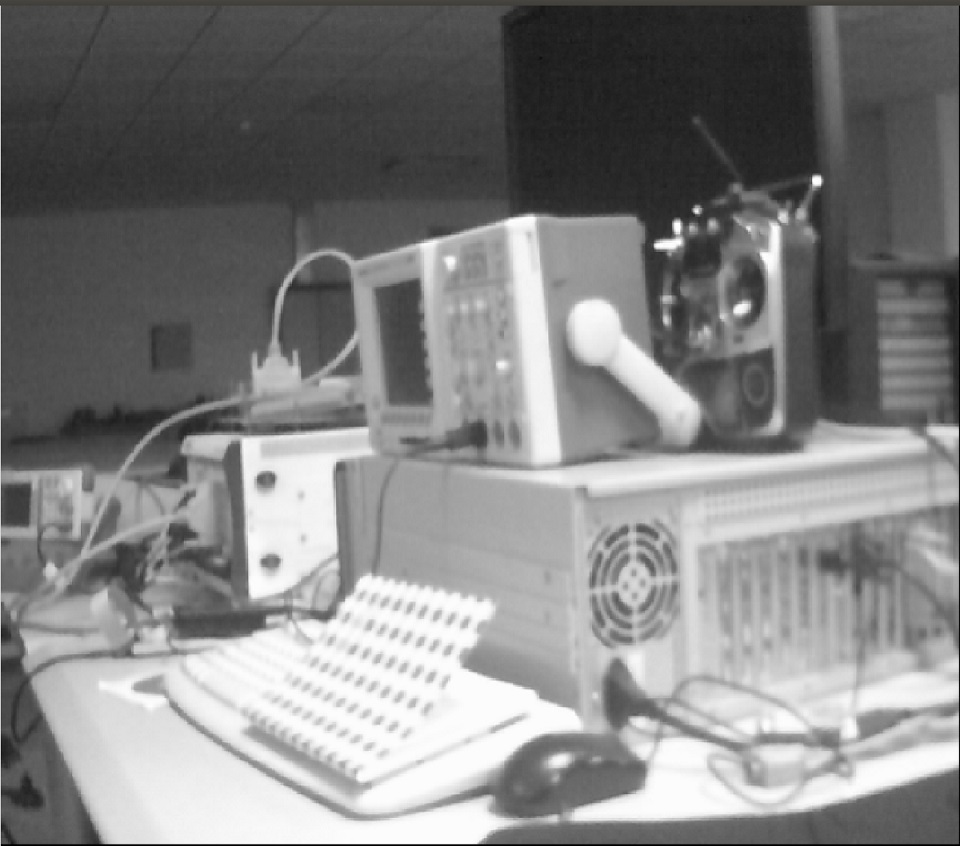
\includegraphics[scale=.2]{figures/Fig4(a)}          
          %\subcaption{}
          }                    
          \subfigure[]
       	  {
          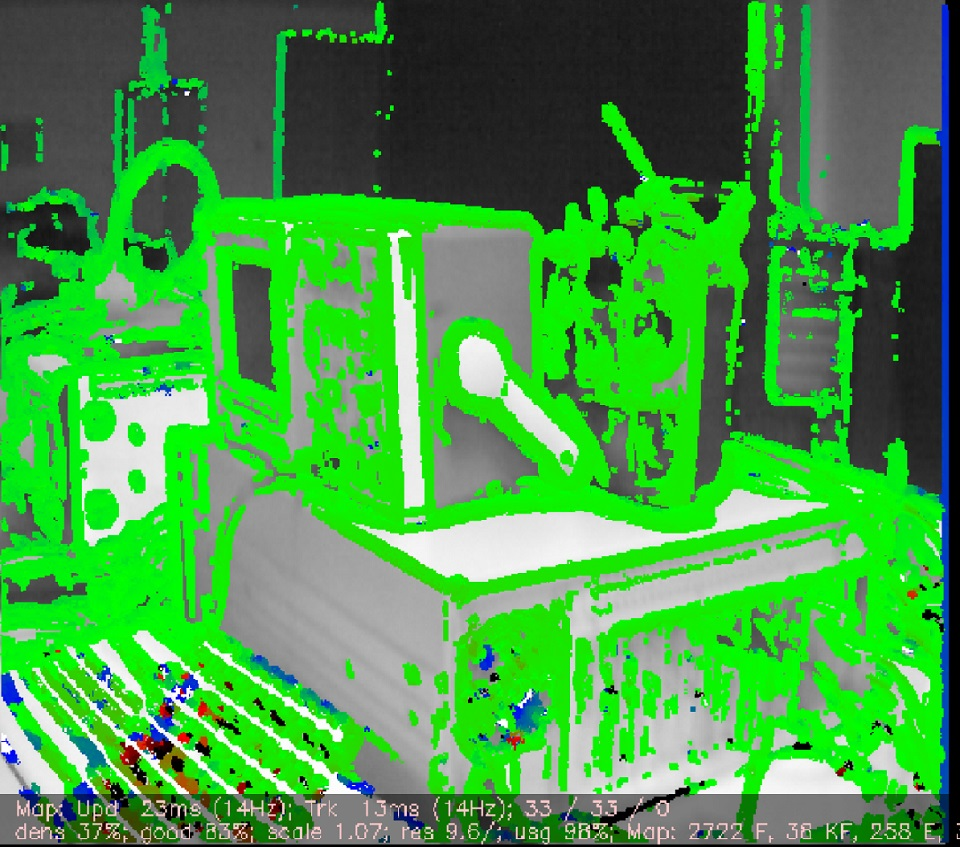
\includegraphics[scale=.2]{figures/Fig4(b)}
          %\subcaption{}
          }
          \hspace{0in}
     
          \subfigure[]
       	  {
          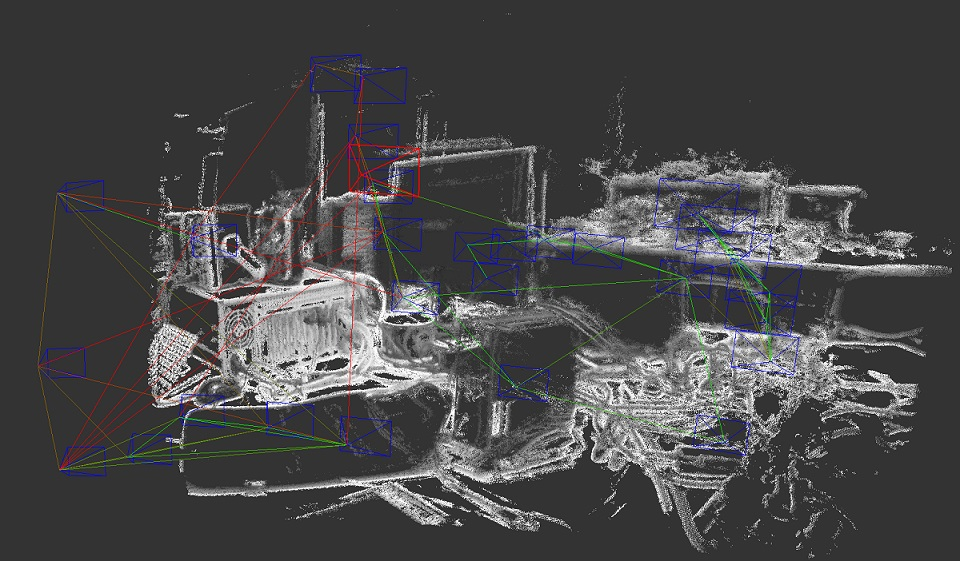
\includegraphics[scale=.25]{figures/Fig4(c)}
          %\subcaption{}
		  }
		  \subfigure[]
       	  {          
          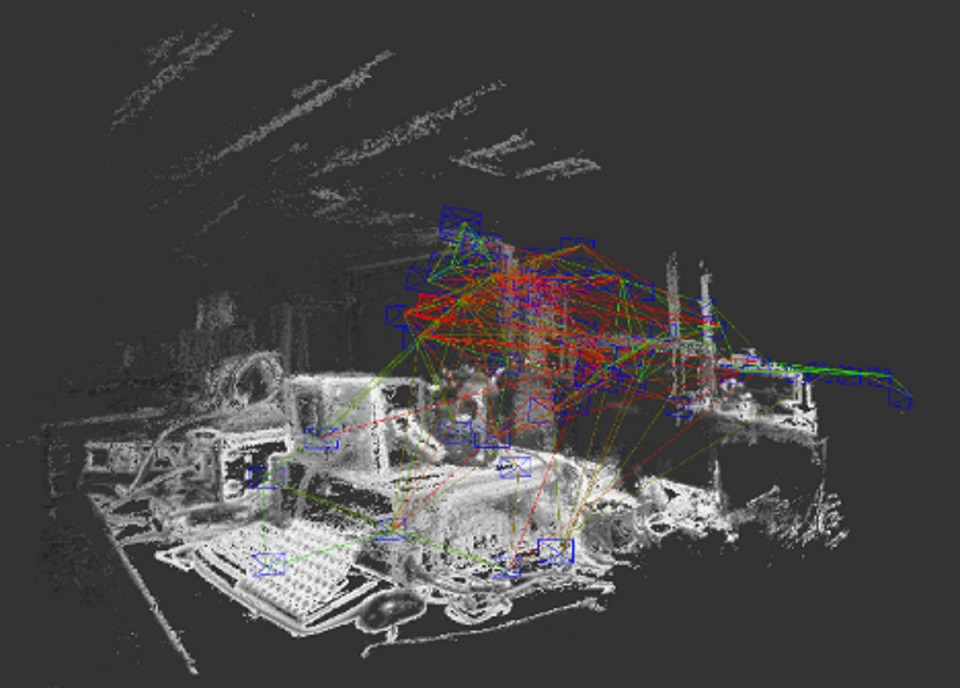
\includegraphics[scale=.2]{figures/Fig4(d)}
          %\subcaption{}
          }
          \hspace{0in}
       %\end{minipage}
     \caption{The indoor LSD-SLAM Map}
\end{figure}

\fi



\iffalse
We evaluate the LSD-SLAM performance in outdoor. We accomplish the reconstruction the 3D map in diverse scene which is different distance. The result is expressed in Fig.5

The picture (a) and (b) are the different distance scene reference image for hand holding camera. The (c) and (d) is the reconstruction map of the LSD-SLAM. We can find that the mapping is completely reconstructed the scene information and the noisy is low in outdoor environment. This can be used in unmanned aerial vehicle(UAV) navigation and localization. The LSD-SLAM is reliable and robustness.

\begin{figure}
    \centering
       %\begin{minipage}{5cm}
       	  \subfigure[]
       	  {
          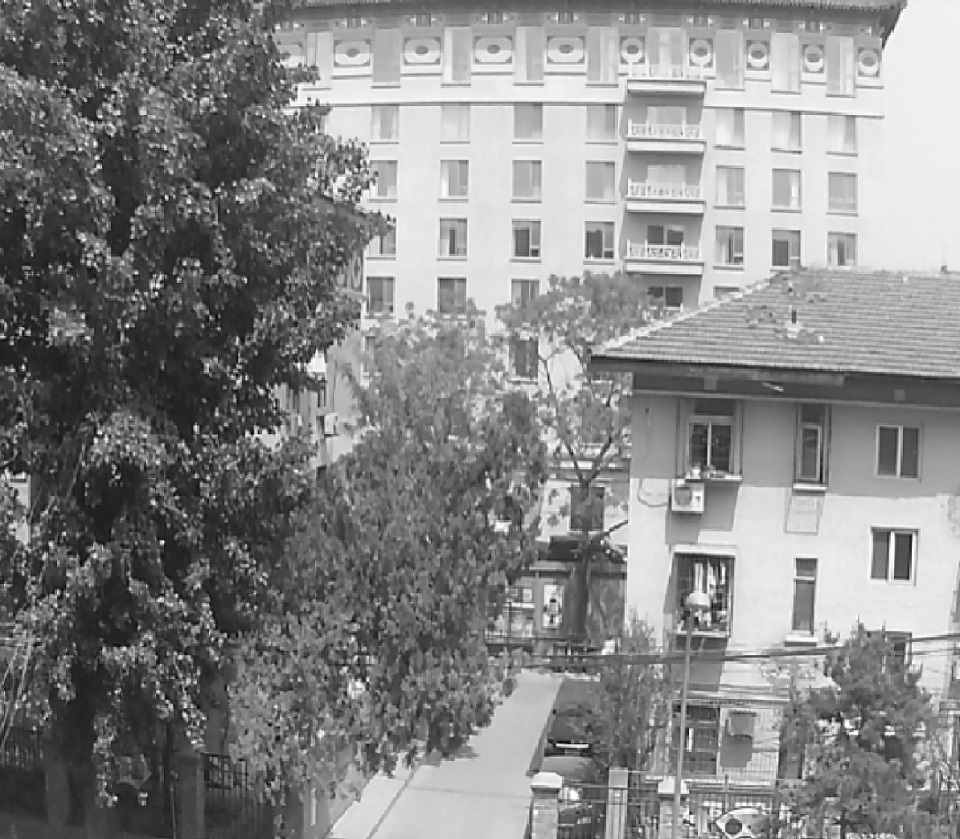
\includegraphics[scale=.2]{figures/Fig5(a)}          
          %\subcaption{}
          }                    
          \subfigure[]
       	  {
          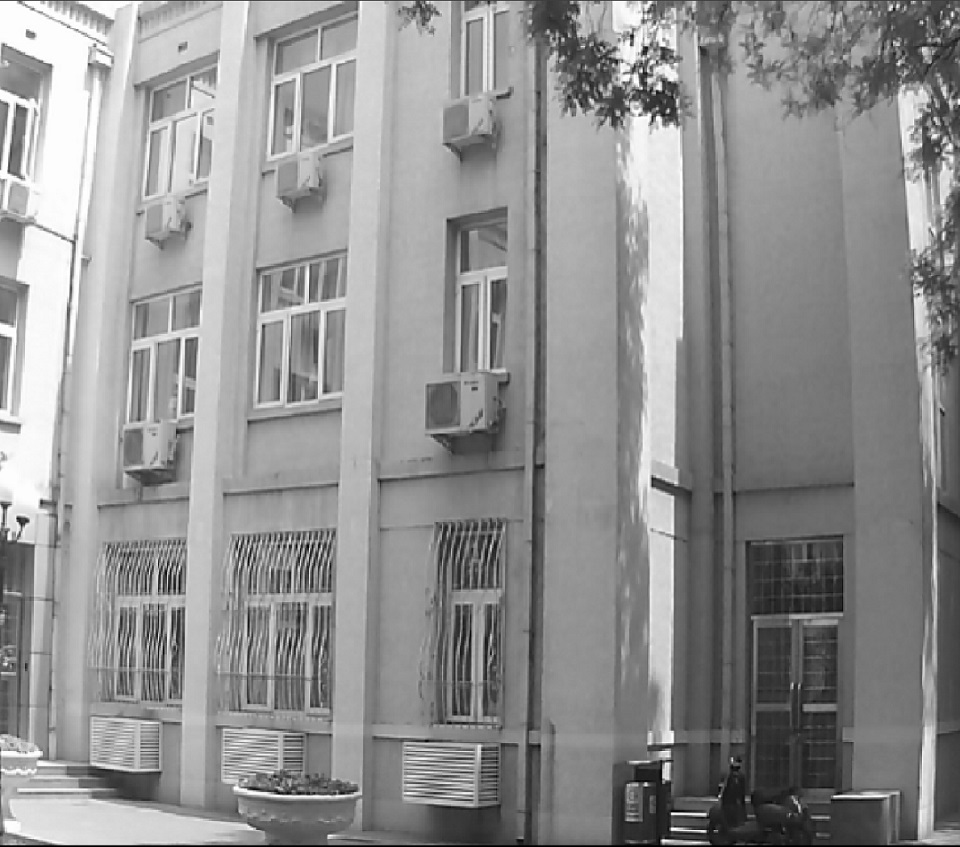
\includegraphics[scale=.2]{figures/Fig5(b)}
          %\subcaption{}
          }
          \hspace{0in}
     
          \subfigure[]
       	  {
          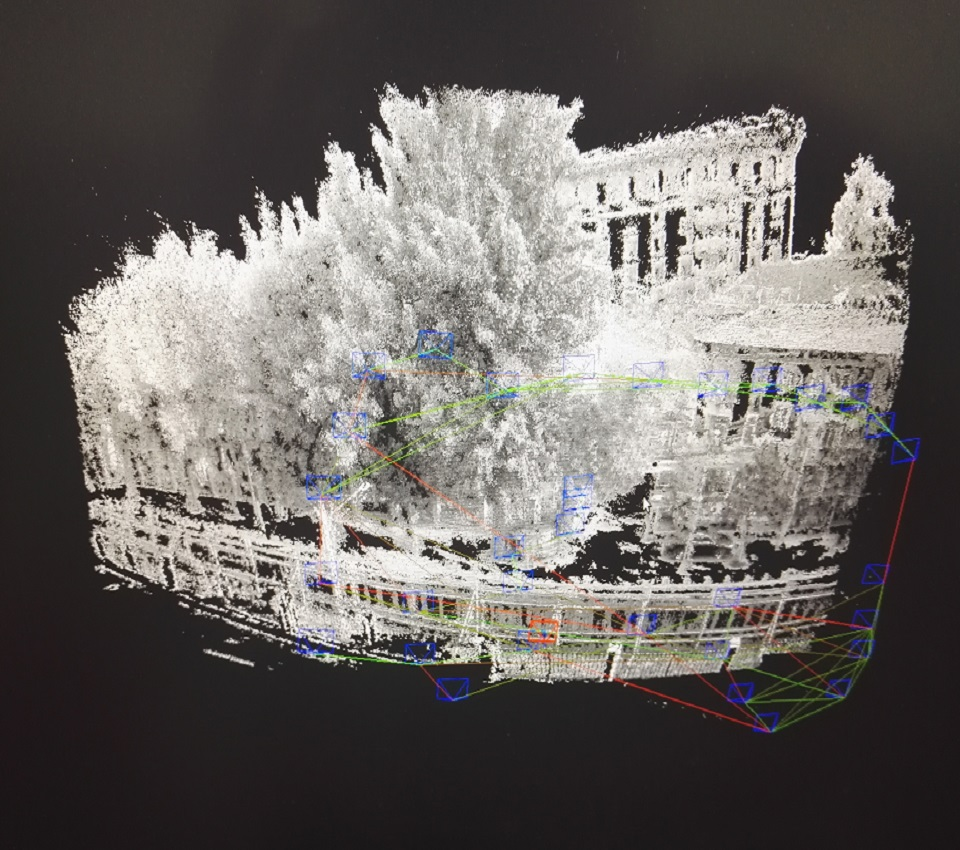
\includegraphics[scale=.25]{figures/Fig5(c)}
          %\subcaption{}
		  }
		  \subfigure[]
       	  {          
          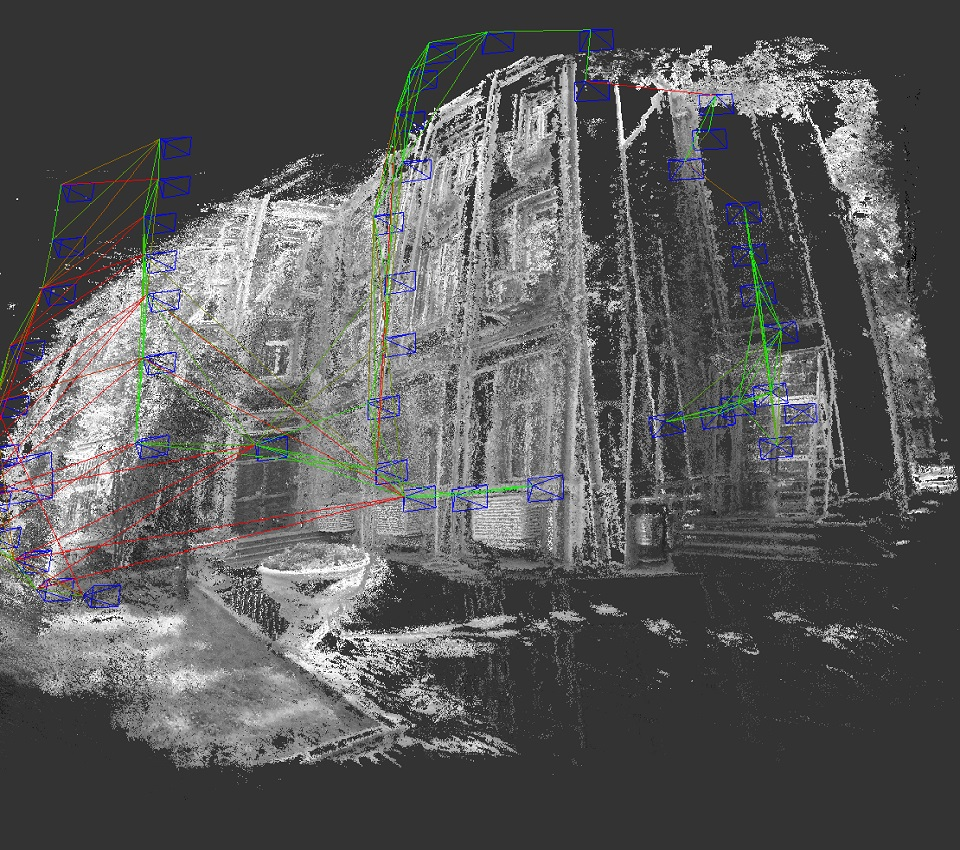
\includegraphics[scale=.2]{figures/Fig5(d)}
          %\subcaption{}
          }
          \hspace{0in}
       %\end{minipage}
     \caption{The outdoor LSD-SLAM Map}
\end{figure}
\fi




\iffalse
\begin{table}
\newcommand{\tabincell}[2]{\begin{tabular}{@{}#1@{}}#2\end{tabular}}
\centering

    \caption{Localization Error in Tum Dataset}     % NOTE!  caption goes _before_ the table contents !!
    \label{tab:font-sizes}
	\renewcommand\arraystretch{1.5}
    \begin{small}
    \begin{tabular}{p{2cm}p{1.5cm}p{1.5cm}p{1.5cm}}
    \hline

    \multicolumn{1}{c}{\multirow{3}{*}{Seq.}}
    & \multicolumn{3} {c} {\bfseries\tabincell{c} {Absolute Key Frame \\ Trajectory RMSE(cm)}} \\
    \cline{2-4}
    \multicolumn{1}{c}{}&   \multicolumn{1}{c}{\bfseries \tabincell{c}{LSD-SLAM} }      &     \multicolumn{1}{c}{\bfseries \tabincell{c}{ semi-dense \\mono-VO}}   & \multicolumn{1}{c}{\bfseries \tabincell{c}{ RGB-D \\SLAM}} \\	

    \cline{1-4}


  \multicolumn{1}{c}{fr2/desk}     &\multicolumn{1}{c}{5.65}      &\multicolumn{1}{c}{13.50}       &\multicolumn{1}{c}{2.58}   \\

  \multicolumn{1}{c}{Fr2/xyz}       &\multicolumn{1}{c}{2.15}      &\multicolumn{1}{c}{3.79}        &\multicolumn{1}{c}{1.34}   \\

  \multicolumn{1}{c}{sim/slowmo}    &\multicolumn{1}{c}{0.37}      &\multicolumn{1}{c}{2.21}        &\multicolumn{1}{c}{0.13}   \\

  \hline

    \end{tabular}
    \end{small}
\end{table}

The LSD-SLAM is evaluated on the Tum dataset. It is very challenging because of containing fast rotational movement, strong motion blur and rolling shutter artifacts. The result is displayed in tableⅠand compared with other algorithm for the localization accuracy.We use the very first depth map to bootstrap the system and get the correct initial scale.

\fi
%%==================================================
%% chapter02.tex for BIT Master Thesis
%% modified by yang yating
%% version: 0.1
%% last update: Dec 25th, 2016

%% modified by Meng Chao
%% version: 0.2
%% last update: May 29th, 2017
%%==================================================
\chapter{基于IMU预积分的惯性视觉单目SLAM算法}
\label{chap:VISLAM}
针对第三章提到的单目SLAM算法缺少场景的尺度信息,鲁棒性较差的问题。本章研究一种基于惯性测量单元(IMU)预积分的惯性-视觉单目SLAM算法,在原有基于特征的ORB-SLAM算法基础上,使用预积分算法对IMU数据进行处理,通过非线性优化将IMU预积分结果与视觉传感器进行融合,获取环境的尺度信息并提高单目SLAM算法的鲁棒性。

IMU与视觉数据融合分为松耦合和紧耦合两种方法。松耦合分别通过IMU和图像估计状态变量,之后通过滤波器进行数据融合;紧耦合则将IMU信息与视觉约束放在统一的非线性优化框架下估计状态变量。使用松耦合滤波方法进行数据融合时,状态变量只包含当前状态,不考虑之前的状态。由于受到线性化误差和计算能力的限制,通常只能构建很少的地图点或者采用无结构化的状态向量对地图点进行边缘化。但由于需要对测量的结构化数据进行延时处理,导致状态更新精度下降,且状态变量的边缘化会产生线性化误差和离群值,容易导致滤波器失效;而采用紧耦合非线性优化进行信息融合,状态向量包含随时间滑动的窗口内多个状态或之前的全部状态,使得状态估计更加准确。同时可以引入鲁邦的优化核函数,降低离群值对状态估计的影响。针对本章中IMU与视觉信息融合,由于IMU频率通常在$100-1000Hz$而图像信息大约在$20-60Hz$,无法每次IMU测量后更新状态变量,引入IMU预积分算法估计关键帧之间IMU信息,将预积分得到的状态信息加入非线性优化框架进行状态估计与更新。


%5.1
\section{基于最大后验的惯性-视觉状态估计}
惯性视觉单目SLAM算法主要是通过捷联的IMU与视觉传感器,估计系统的位姿、速度与环境地图点的位置。假设IMU坐标系用$B$表示,相机坐标系用$C$表示,通过预先标定得到相机坐标系到IMU坐标系的坐标变换$\boldsymbol{T}_{BC}$,如图\ref{fig5.1}所示。
\begin{figure}
\centering
%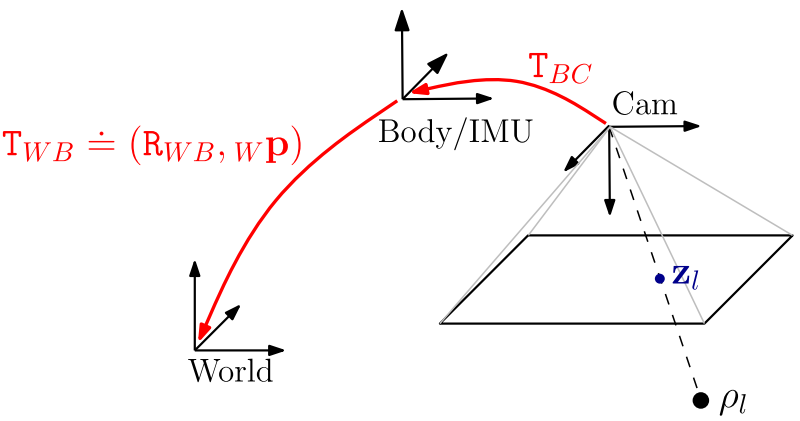
\includegraphics[scale=0.4]{figures/Fig5.1.png}
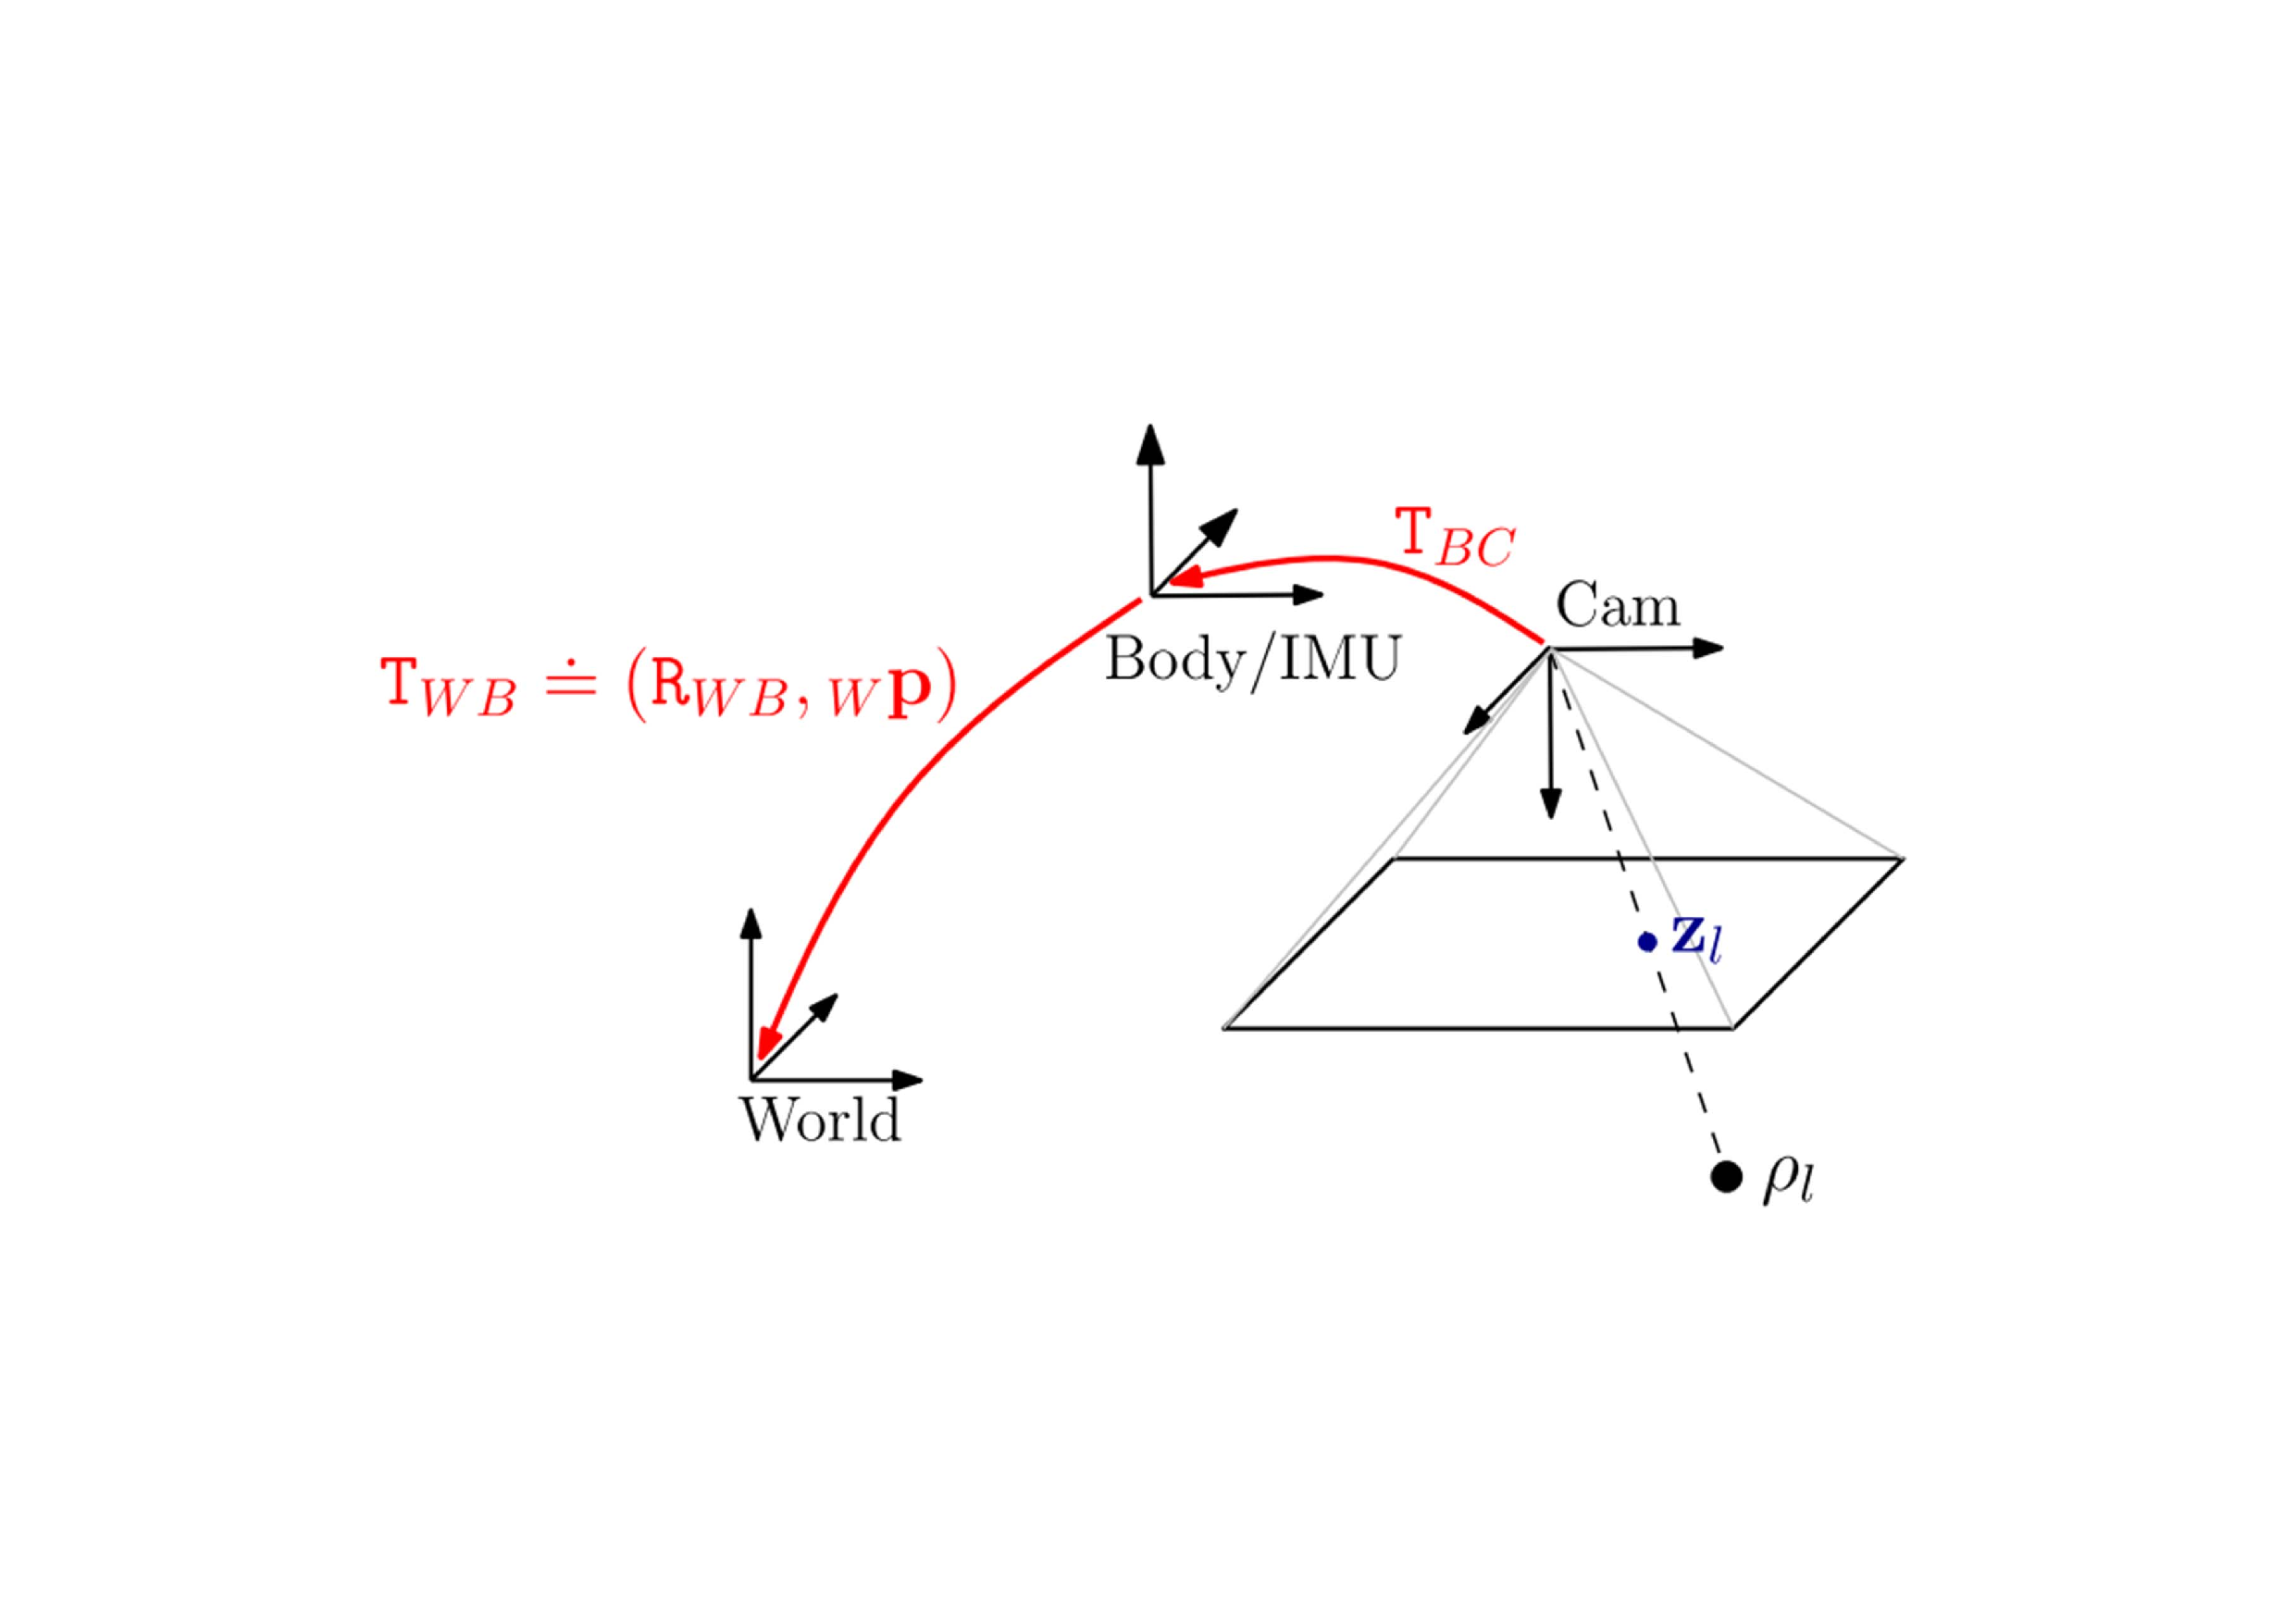
\includegraphics[scale=0.35,angle=-90]{figures/Fig5-1.pdf}
\caption{IMU-相机坐标系变换}
\label{fig5.1}
\end{figure}

在惯性视觉单目SLAM算法中,系统的状态变量可以表示为姿态,位置,速度,IMU偏移
\begin{equation}
\label{equ5.1}
\boldsymbol{x}_i \doteq \left[ \boldsymbol{R}_i,\boldsymbol{p}_i,\boldsymbol{v}_i,\boldsymbol{b}_i \right]
\end{equation}
其中位姿表示在李群$SE(3)$空间下,记作$\left( \boldsymbol{R}_i, \boldsymbol{p}_i \right)$;速度表示在欧式向量空间,记作$\boldsymbol{v}_i \in \mathds{R}^3 $;IMU偏移表示在欧式向量空间下,记作$\boldsymbol{b}_i=[\boldsymbol{b}_i^g \ \boldsymbol{b}_i^a] \in \mathds{R}^6$。

如第三章所述,SLAM问题可以抽象为基于最大后验的状态估计问题。记$k$时刻之前的所有关键帧的集合为$\mathcal{K}_k$,所有关键帧对应状态变量的集合表示为$\mathcal{X}_k \doteq \{\boldsymbol{x}_i\}_{i \in \mathcal{K}_k}$。与纯视觉SLAM问题不同,在惯性视觉单目SLAM算法中输入不仅包括相机图像,还有IMU测量值。第$i$时刻的关键帧图像为$C_i$,图像$C_i$中包括多个地图点$l$在第$i$时刻对应的观测值$z_{il}$。从第$i$时刻到第$j$时刻的两连续关键帧之间的IMU测量值集合为$\mathcal{I}_{ij}$。则$k$时刻之前系统的观测量的集合表示为
\begin{equation}
\label{equ5.2}
Z_k \doteq \{C_i,\mathcal{I}_{ij}\}_{(i,j) \in \mathcal{K}_k}
\end{equation}

将第三章中关于视觉SLAM算法的最大后验状态估计的方法推广到惯性视觉单目SLAM算法中,在给定相机和IMU观测量$Z_k$与先验$p(\mathcal{X}_0)$的情况下,有
\begin{equation}
\label{equ5.3}
\begin{aligned}
p(\mathcal{X}_k | Z_k) & \varpropto p(\mathcal{X}_0)p(Z_k | \mathcal{X}_k) = p(\mathcal{X}_0) \prod\limits_{(i,j) \in \mathcal{K}_k} p \left( C_i,\mathcal{I}_{ij} | \mathcal{X}_k \right) \\
&=p(\mathcal{X}_0) \prod\limits_{(i,j) \in \mathcal{K}_k} p \left( \mathcal{I}_{ij} | x_i,x_j \right) \prod\limits_{i \in \mathcal{K}_k} \prod\limits_{l \in C_i}  p \left( z_{il} | x_i \right)
\end{aligned}
\end{equation}

由于最大后验估计与最小负对数后验估计等价,在传感器观测服从零偏高斯噪声的情况下,对状态变量$\mathcal{X}_k^*$的最大后验估计可以表示为
\begin{equation}
\label{equ5.4}
\begin{aligned}
\mathcal{X}_k^* & = \argmin\limits_{\mathcal{X}_k}- \log_e p(\mathcal{X}_k | Z_k) \\ 
& = \argmin\limits_{\mathcal{X}_k} \left\Vert \boldsymbol{r}_0 \right\Vert_{\boldsymbol{\Sigma}_0}^2+ \sum\limits_{(i,j) \in \mathcal{K}_k}\left\Vert \boldsymbol{r}_{\mathcal{I}_{ij}} \right\Vert_{\boldsymbol{\Sigma}_{ij}}^2+ \sum\limits_{i \in \mathcal{K}_k}\sum\limits_{l \in \mathcal{C}_i} \left\Vert \boldsymbol{r}_{C_{il}} \right\Vert_{\boldsymbol{\Sigma}_{C}}^2
\end{aligned}
\end{equation}
其中$\boldsymbol{r}_0$,$ \boldsymbol{r}_{\mathcal{I}_{ij}}$,$\boldsymbol{r}_{C_{il}}$表示与测量值相关的残差,$\boldsymbol{\Sigma}_0$,$ \boldsymbol{\Sigma}_{ij}$,$\boldsymbol{\Sigma}_C$表示残差对应的协方差矩阵。残差是关于状态变量$\mathcal{X}_k$的方程,用于表示测量值与状态变量$\mathcal{X}_k$给定情况下的预测值之间的误差。公式\eqref{equ5.4}将惯性视觉SLAM问题抽象为关于状态变量$\mathcal{X}_k$的最优估计问题,本章之后的内容介绍如何构建最优估计的目标函数约束和协方差矩阵,将IMU数据耦合到原有的视觉SLAM算法图优化框架中。


%5.2
\section{IMU预积分算法}

\subsection{IMU模型与运动估计}
惯性测量单元(IMU)一般由三轴加速度计和三轴陀螺仪组成,测量传感器相对于惯性坐标系的旋转角速率和加速度。IMU的测量值$\widetilde{\boldsymbol{a}}_B(t)$,$\widetilde{\boldsymbol{\omega}}_{W\!B}(t)$受高斯白噪声$\eta$和传感器偏移$b$的影响,IMU传感器模型如方程\eqref{equ5.5}
\begin{equation}
\label{equ5.5}
\begin{aligned}
\widetilde{\boldsymbol{\omega}}_{W\!B}(t) &= \boldsymbol{\omega}_{W\!B}(t)+\boldsymbol{b}^g(t)+\boldsymbol{\eta}^g(t) \\
\widetilde{\boldsymbol{a}}_B(t) &= \boldsymbol{R}_{W\!B}^T(t)(\boldsymbol{a}_W(t)-\boldsymbol{g}_w)+\boldsymbol{b}^a(t)+\boldsymbol{\eta}^a(t)
\end{aligned}
\end{equation}
其中$\boldsymbol{\omega}_{W\!B}(t) \in \mathds{R}^3$表示在IMU坐标系下IMU坐标系相对于世界坐标系的旋转角速率,$\boldsymbol{a}_W(t) \in \mathds{R}^3$表示相对于世界坐标系下的测量加速度,$\boldsymbol{R}_{W\!B}$表示从IMU坐标系到世界坐标的相对旋转。

为了获取IMU测量的运动信息,根据体动力学模型
\begin{equation}
\label{equ5.6}
\begin{aligned}
\dot{\boldsymbol{R}}_{W\!B} &= \boldsymbol{R}_{W\!B}{\boldsymbol{\omega}}_{W\!B}^{\wedge}\\
\dot{\boldsymbol{v}}_W &= \boldsymbol{a}_W \\
\dot{\boldsymbol{p}}_W &= \boldsymbol{v}_W
\end{aligned}
\end{equation}
其中,${\boldsymbol{\omega}}_{W\!B}^{\wedge}$表示角速率向量的旋转矩阵。对公式\eqref{equ5.6}积分可以得到在$t+\Delta t$时刻的运动状态为
\begin{equation}
\label{equ5.7}
\begin{aligned}
\boldsymbol{R}_{W\!B}(t+\Delta t) &= \boldsymbol{R}_{W\!B}(t)\exp\left( { \left( \int_t^{t+\Delta t} \! \boldsymbol{\omega}_{W\!B}(\tau) d\tau \right)^{\wedge} } \right) \\
\boldsymbol{v}_W(t+\Delta t) &= \boldsymbol{v}_W(t) + \int_t^{t+\Delta t} \! \boldsymbol{a}_W(\tau) d\tau 
\\
\boldsymbol{p}_W(t+\Delta t) &= \boldsymbol{p}_W(t) + \int_t^{t+\Delta t} \! \boldsymbol{v}_W(\tau) d\tau + \iint_t^{t+\Delta t} \! \boldsymbol{a}_W(\tau)d\tau ^2
\end{aligned}
\end{equation}
假设在$t$到$t+\Delta t$时间段内$\boldsymbol{a}_W$和$\boldsymbol{\omega}_{W\!B}$为常量,则公式\eqref{equ5.7}可以表示为
\begin{equation}
\label{equ5.8}
\begin{aligned}
\boldsymbol{R}_{W\!B}(t+\Delta t) &= \boldsymbol{R}_{W\!B}(t) \exp(( \boldsymbol{\omega}_{W\!B}(t)\Delta t )^{\wedge}) \\
\boldsymbol{v}_W(t+\Delta t) &= \boldsymbol{v}_W(t)+\boldsymbol{a}_W(t)\Delta t \\
\boldsymbol{p}_W(t+\Delta t) &= \boldsymbol{p}_W(t)+\boldsymbol{v}_W(t)\Delta t + {1 \over 2} \boldsymbol{a}_W(t)\Delta t^2
\end{aligned}
\end{equation}
将方程\eqref{equ5.5}带入方程\eqref{equ5.8},可以得到运动状态关于IMU测量值$\widetilde{\boldsymbol{\omega}}_{W\!B}$,$\widetilde{\boldsymbol{a}}_B$的函数
\begin{equation}
\label{equ5.9}
\begin{aligned}
\boldsymbol{R}(t+\Delta t) &= \boldsymbol{R}(t)\exp \left( \left(  \left( \widetilde{\boldsymbol{\omega}}_{W\!B}(t)-\boldsymbol{b}^g(t)-\boldsymbol{\eta}^{gd}(t) \right) \Delta t \right)^{\wedge}  \right) \\ 
\boldsymbol{v}(t+\Delta t) &= \boldsymbol{v}(t)+\boldsymbol{g} \Delta t + \boldsymbol{R}(t)(\widetilde{\boldsymbol{a}}(t)-\boldsymbol{b}^a(t)-\boldsymbol{\eta}^{ad}(t))\Delta t \\
\boldsymbol{p}(t+\Delta t) &= \boldsymbol{p}(t)+\boldsymbol{v}(t)\Delta t + {1 \over 2}\boldsymbol{g}\Delta t^2 + {1 \over 2}\boldsymbol{R}(t)(\widetilde{\boldsymbol{a}}(t)-\boldsymbol{b}^a(t)-\boldsymbol{\eta}^{ad}(t))\Delta t^2
\end{aligned}
\end{equation}
为了便于表示,省略方程\eqref{equ5.9}状态变量的坐标系下标。在速度和位置的数值积分中,假设两次测量之间的旋转矩阵$R(t)$为常量,虽然方程\eqref{equ5.9}不是方程\eqref{equ5.7}的精确解,但在IMU采样频率较高时可以认为近似精度足够高,因而在实际应用中采取以上模型近似求解。如果IMU采样速率较低,可以考虑采用更为准确的数值积分近似方法。

\subsection{IMU预积分观测模型}
方程\eqref{equ5.9}可以作为\eqref{equ5.4}最大后验图优化框架的约束,但其中包含需要频繁更新的状态变量。此外,方程\eqref{equ5.9}中涉及到时间$t$和$t+\Delta t$的状态,因此在每次得到新的IMU测量时需要增加状态变量。针对以上问题,采用IMU预积分算法,将连续两帧关键帧之间的IMU观测数据整合为一个包含运动状态的测量信息,如图\ref{fig5.2}所示。
\begin{figure}
\centering
%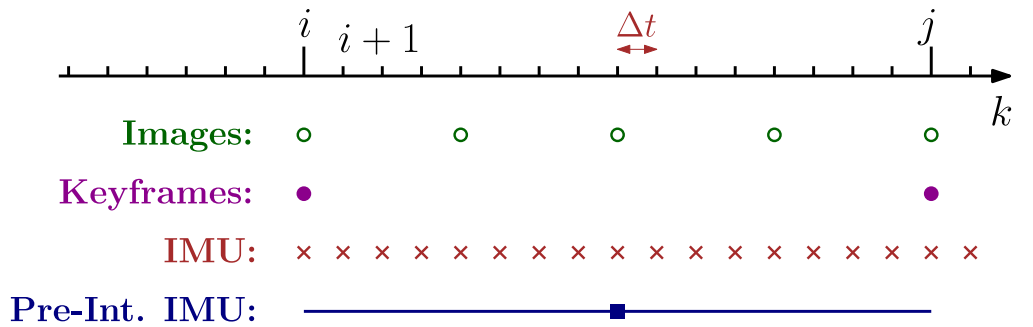
\includegraphics[scale=0.4]{figures/Fig5.2.png}
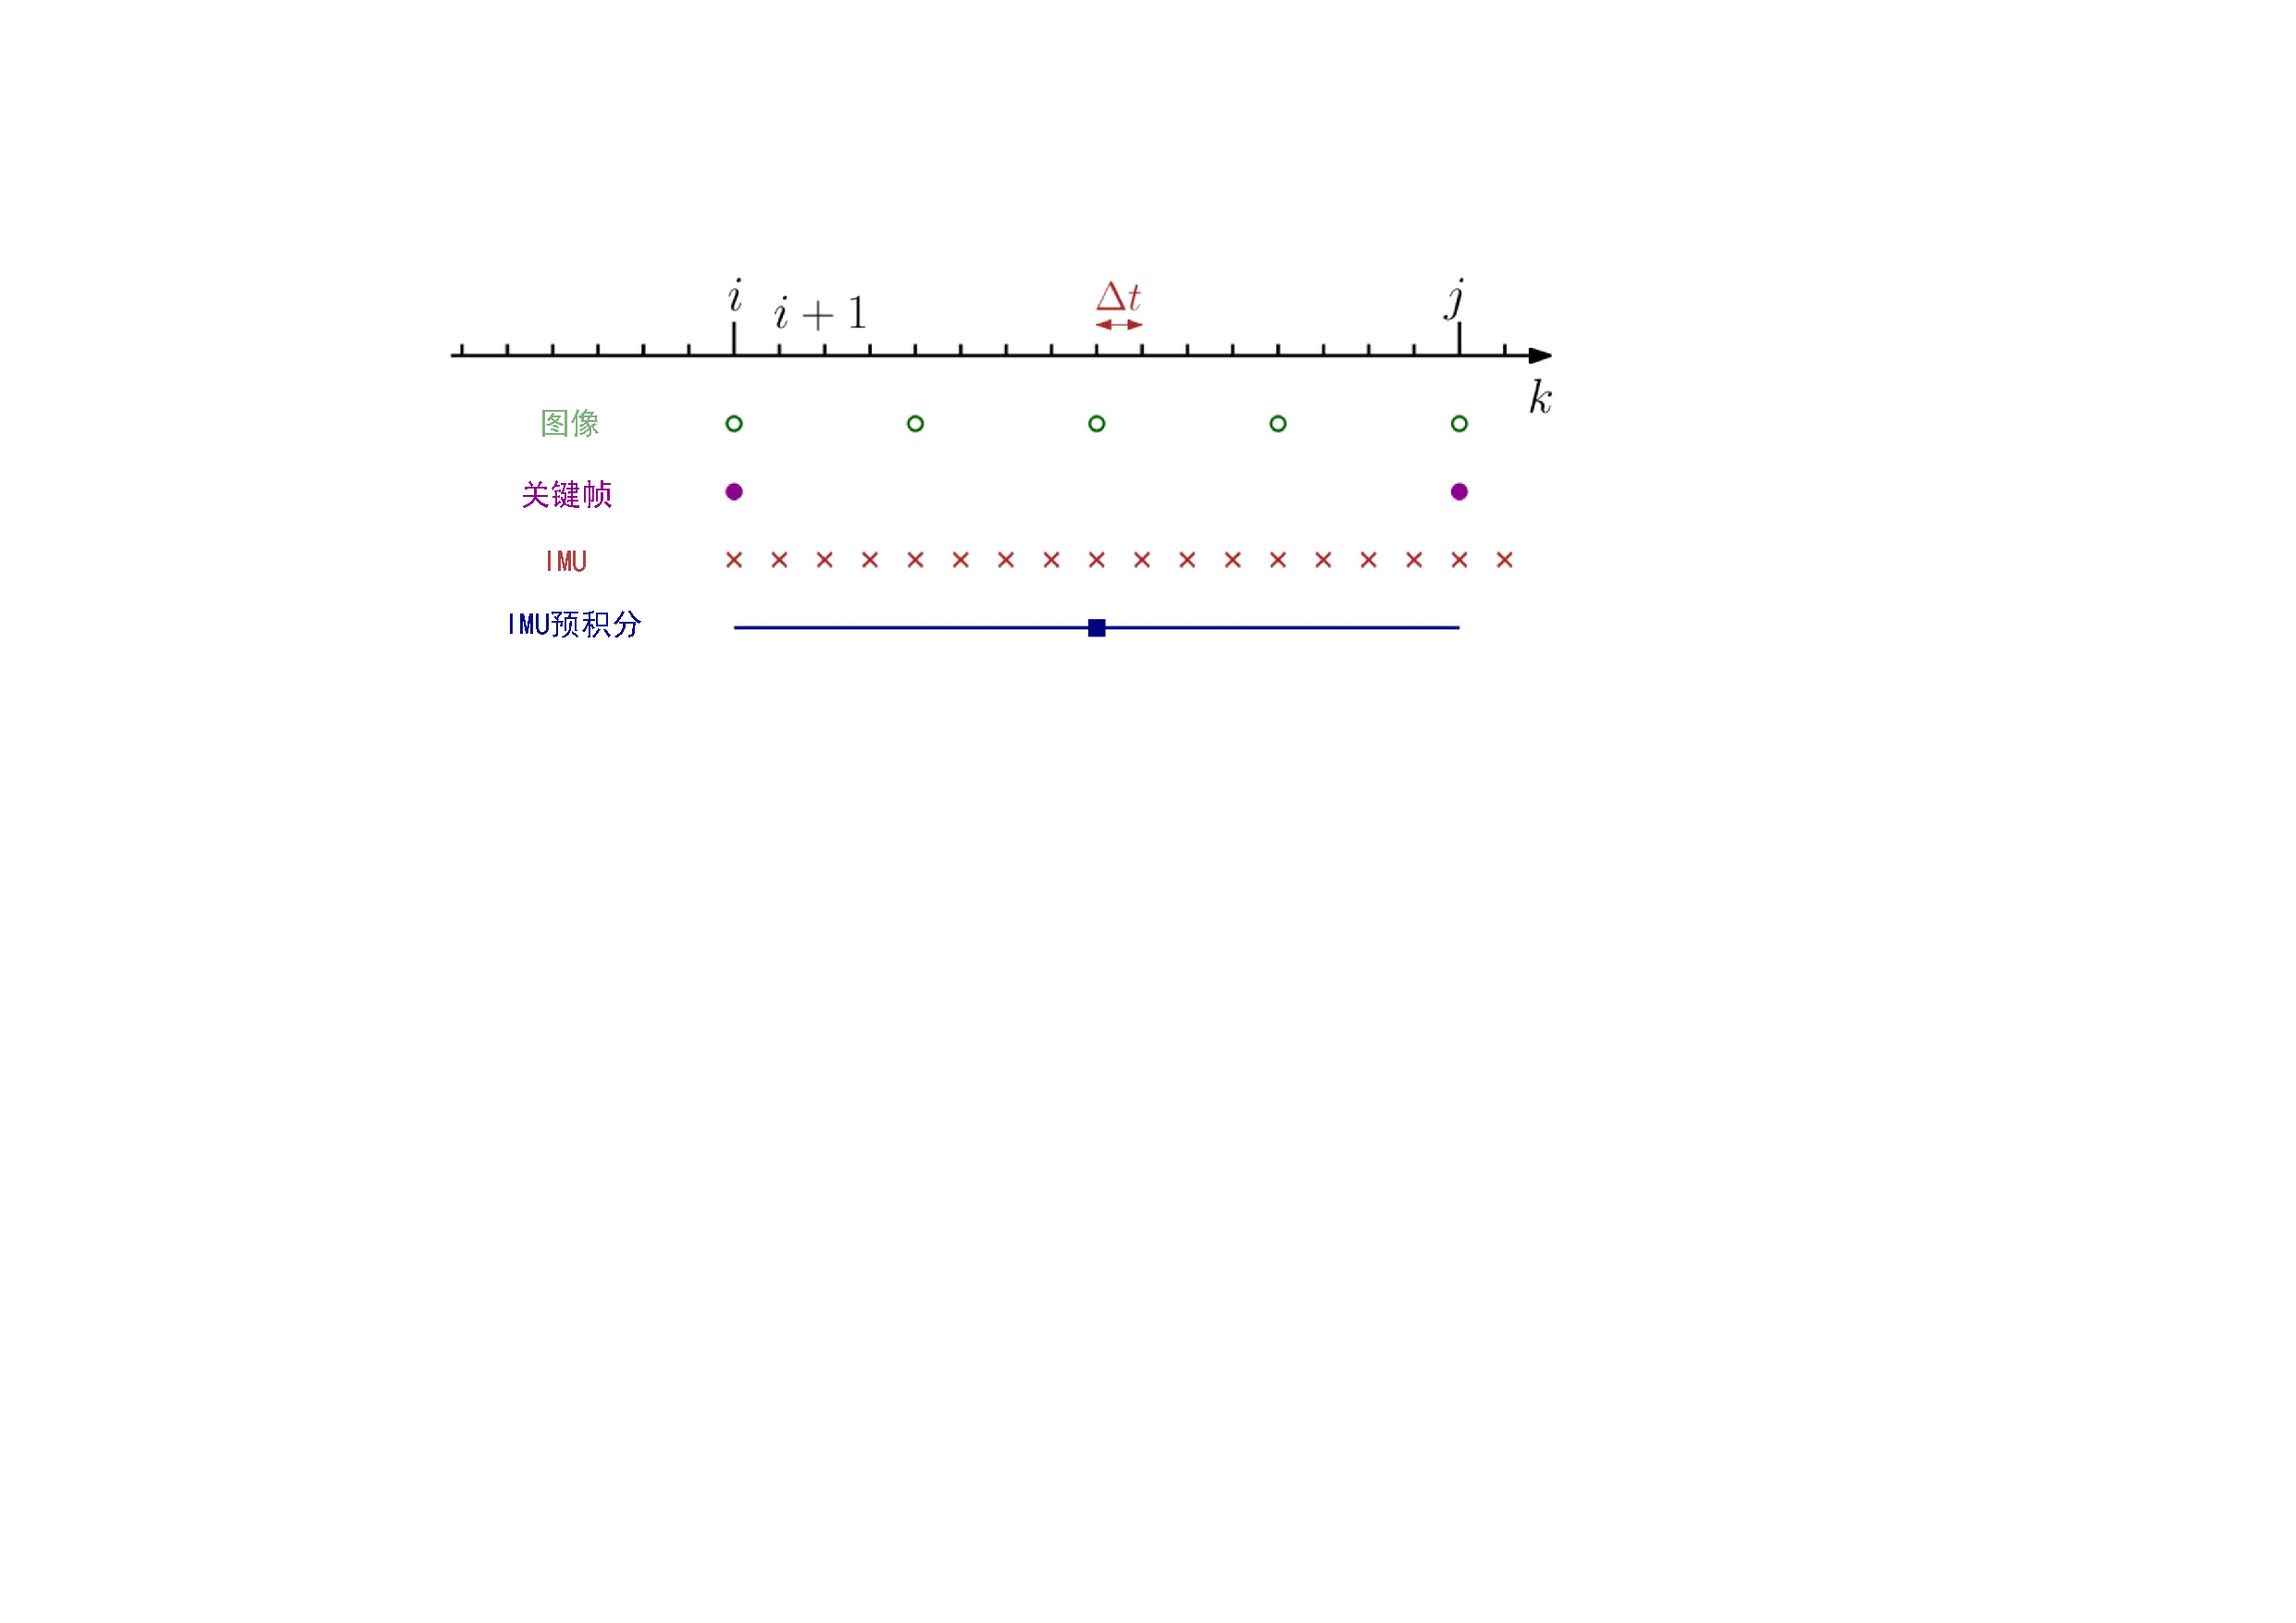
\includegraphics[scale=0.6,angle=-90]{figures/Fig5-2.pdf}
\caption{IMU预积分示意图}
\label{fig5.2}
\end{figure}

假设IMU测量数据与相机图像经过同步处理,对两连续关键帧$i$与$j$之间的所有采样间隔$\Delta t$上的IMU测量数据通过方程\eqref{equ5.9}进行迭代,可以得到
\begin{equation}
\label{equ5.10}
\begin{aligned}
\boldsymbol{R}_j &= \boldsymbol{R}_i \prod\limits_{k=i}^{j-1}\exp \left( \left( \left( \widetilde{\boldsymbol{\omega}}_k - \boldsymbol{b}_k^g-\boldsymbol{\eta}_k^{gd} \right) \Delta t \right)^{\wedge} \right) 
\\ 
\boldsymbol{v}_j &= \boldsymbol{v}_i+\boldsymbol{g} \Delta t_{ij} +  \sum\limits_{k=i}^{j-1}R_k \left( \widetilde{\boldsymbol{a}}_k - \boldsymbol{b}_k^a -\boldsymbol{\eta}_k^{ad} \right)\Delta t
\\
\boldsymbol{p}_j &= \boldsymbol{p}_i + \sum\limits_{k=i}^{j-1} \left[ \boldsymbol{v}_k \Delta t + {1 \over 2}\boldsymbol{g}\Delta t^2 + {1 \over 2}\boldsymbol{R}_k \left( \widetilde{\boldsymbol{a}}_k - \boldsymbol{b}_k^a -\boldsymbol{\eta}_k^{ad} \right)\Delta t^2 \right]
\end{aligned}
\end{equation}
为了便于表示,$(\cdot)_i \doteq (\cdot)(t_i)$,关键帧$i$,$j$之间的时间间隔$\Delta t_{ij} = \sum_{k=i}^{j-1}\Delta t$。方程\eqref{equ5.10}可以用于估计$t_i$到$t_j$时刻之间的运动,但是当方程中的线性化点$t_i$发生变化后,需要重新计算IMU运动信息的数值积分。例如,当姿态$R_i$变化后,从$k=i,...j-1$的所有时刻的姿态,速度和位置都需要重新计算。为了避免重复计算,对方程\eqref{equ5.10}进行变化,定义与$t_i$时刻的位姿和速度无关的相对运动增量
\begin{equation}
\label{equ5.11}
\begin{aligned}
\Delta \boldsymbol{R}_{ij} &\doteq \boldsymbol{R}_i^T \boldsymbol{R}_j = \prod\limits_{k=i}^{j-1}\exp \left( \left( \left( \widetilde{\boldsymbol{\omega}}_k - \boldsymbol{b}_k^g-\boldsymbol{\eta}_k^{gd} \right) \Delta t  \right)^{\wedge} \right) 
\\ 
\Delta \boldsymbol{v}_{ij} &\doteq R_i^T\left( \boldsymbol{v}_j-\boldsymbol{v}_i-\boldsymbol{g}\Delta t_{ij}\right) =  \sum\limits_{k=i}^{j-1} \Delta \boldsymbol{R}_{ik} \left( \widetilde{\boldsymbol{a}}_k - \boldsymbol{b}_k^a -\boldsymbol{\eta}_k^{ad} \right)\Delta t
\\ 
\Delta \boldsymbol{p}_{ij} &\doteq \boldsymbol{R}_i^T \left( \boldsymbol{p}_j-\boldsymbol{p}_i-\boldsymbol{v}_i\Delta  t_{ij} - {1 \over 2} \sum\limits_{k=i}^{j-1} \boldsymbol{g} \Delta t^2 \right) \\
&=  \sum\limits_{k=i}^{j-1} \left[ \Delta \boldsymbol{v}_{ik} \Delta t + {1 \over 2}\Delta \boldsymbol{R}_{ik} \left( \widetilde{\boldsymbol{a}}_k - \boldsymbol{b}_k^a -\boldsymbol{\eta}_k^{ad} \right)\Delta t^2 \right]
\end{aligned}
\end{equation}
其中$\boldsymbol{R}_{ik} \doteq \boldsymbol{R}_i^T \boldsymbol{R}_k$,$\Delta \boldsymbol{v}_{ik} \doteq \boldsymbol{R}_i^T \left( \boldsymbol{v}_k -\boldsymbol{v}_i-\boldsymbol{g}\Delta t_{ik} \right)$。在方程\eqref{equ5.11}中,不同于相对姿态增量$\Delta \boldsymbol{R}_{ij}$,$\Delta \boldsymbol{v}_{ij}$和$\Delta \boldsymbol{p}_{ij}$与实际物理世界中的速度和位置增量并不对应。但这样定义可以使方程\eqref{equ5.11}中$\Delta \boldsymbol{R}_{ij}$,$\Delta \boldsymbol{v}_{ij}$和$\Delta \boldsymbol{p}_{ij}$的右侧表达式直接通过IMU的测量值计算得,而不受$i$时刻的状态和重力加速$\boldsymbol{g}$的影响,避免重复计算。

虽然方程\eqref{equ5.11}可以避免重复计算,但是在每次计算相对状态时,仍需要考虑IMU传感器的偏移$b_i$。在本节之后的推到中,先假设连续两连续关键帧之间的IMU偏移为常量,在下一节中考虑当IMU传感器偏移变化后相对运动增量的补偿。
\begin{equation}
\label{equ5.12}
\boldsymbol{b}_i^g = \boldsymbol{b}_{i+1}^g = \cdots = \boldsymbol{b}_{j-1}^g, \  \boldsymbol{b}_i^a = \boldsymbol{b}_{i+1}^a = \cdots = \boldsymbol{b}_{j-1}^a
\end{equation}

方程\eqref{equ5.11}将关键帧$i$,$j$之间的相对状态(等号左侧)和IMU传感器的测量值(等号右侧)相关联,因而可以将方程\eqref{equ5.11}看做IMU传感器的观测模型。但是,该模型在当前的表示形式下,其观测噪声的不确定性分析较为复杂,无法获取该模型应用于最大后验估计所需要的概率密度函数表达。因而对方程\eqref{equ5.11}进行变换,根据李群与李代数之间的映射关系和性质(见附录),方程\eqref{equ5.11}中IMU旋转观测模型可以表示为
\begin{equation}
\label{equ5.13}
\begin{aligned}
\Delta \boldsymbol{R}_{ij} & \simeq \prod\limits_{k=i}^{j-1} \left[ \exp \left( \left( \left( \widetilde{\boldsymbol{\omega}}_k - \boldsymbol{b}_i^g \right) \Delta t \right)^{\wedge}  \right)  
\exp \left( \left( -J_r^k \boldsymbol{\eta}_k^{gd} \Delta t \right)^{\wedge} \right)\right] \\
&= \Delta \widetilde{\boldsymbol{R}}_{ij} \prod\limits_{k=i}^{j-1}\exp \left( -\Delta \widetilde{\boldsymbol{R}}_{k+1j}^T \left( J_r^k \boldsymbol{\eta}_k^{gd} \Delta t \right)^{\wedge}  \right) \\ 
& \doteq \Delta \widetilde{\boldsymbol{R}}_{ij} \exp \left(  -\delta \boldsymbol{\phi}_{ij} ^{\wedge}  \right)
\end{aligned}
\end{equation}
其中$J_r^k \doteq J_r^k( \left( \widetilde{\boldsymbol{\omega}}_k - \boldsymbol{b}_i^g \right) \Delta t)$,定义IMU旋转预积分为$\Delta \widetilde{\boldsymbol{R}}_{ij} \doteq \prod_{k=i}^j\exp \left( \left( \left( \widetilde{\boldsymbol{\omega}}_k - \boldsymbol{b}_i^g \right) \Delta t \right)^{\wedge}  \right)$,观测模型中的旋转观测噪声为$\delta \boldsymbol{\phi}_{ij}$。

将方程\eqref{equ5.13}带入方程\eqref{equ5.11},利用李代数指数映射的一阶近似(见附录)展开$\exp \left(  -\delta \boldsymbol{\phi}_{ij}^{\wedge}  \right)$,忽略高阶噪声项,则方程\eqref{equ5.11}中的IMU速度观测模型可以表示为
\begin{equation}
\label{equ5.14}
\begin{aligned}
\Delta \boldsymbol{v}_{ij} & \simeq \sum\limits_{k=i}^{j-1} \Delta \widetilde{\boldsymbol{R}}_{ik}\left( \boldsymbol{I}-\delta \boldsymbol{\phi}_{ik}^{\wedge} \right) \left( \widetilde{\boldsymbol{a}}_k - \boldsymbol{b}_i^a \right) \Delta t -\Delta \widetilde{\boldsymbol{R}}_{ik} \boldsymbol{\eta}_k^{ad} \Delta t 
\\ 
& = \Delta \widetilde{\boldsymbol{v}}_{ij} + \sum\limits_{k=i}^{j-1} \left[ \Delta \widetilde{\boldsymbol{R}}_{ik} \left( \widetilde{\boldsymbol{a}}_k - \boldsymbol{b}_i^a \right)^{\wedge} \delta \boldsymbol{\phi}_{ik} \Delta t - \Delta \widetilde{\boldsymbol{R}}_{ik} \boldsymbol{\eta}_k^{ad} \Delta t \right] \\ 
& \doteq  \Delta \widetilde{\boldsymbol{v}}_{ij} - \delta \boldsymbol{v}_{ij}
\end{aligned}
\end{equation}
其中定义IMU的速度预积分为$\Delta \widetilde{\boldsymbol{v}}_{ij} \doteq \sum_{k=i}^{j-1} \Delta \widetilde{\boldsymbol{R}}_{ik} \left( \widetilde{\boldsymbol{a}}_k - \boldsymbol{b}_i^a \right) \Delta t $,IMU速度观测模型的观测噪声为$\delta \boldsymbol{v}_{ij}$。

同理,将方程\eqref{equ5.13},\eqref{equ5.14}带入方程\eqref{equ5.11},利用李代数指数映射的一阶近似,忽略高阶噪声项,则方程\eqref{equ5.11}中的IMU位置观测模型可以表示为
\begin{equation}
\label{equ5.15}
\begin{aligned} 
\Delta \boldsymbol{p}_{ij} & \simeq \sum\limits_{k=i}^{j-1} \left[ (\Delta \widetilde{\boldsymbol{v}}_{ik} - \delta \boldsymbol{v}_{ik}) \Delta t + {1 \over 2} \Delta \widetilde{\boldsymbol{R}}_{ik}\left( \boldsymbol{I}-\delta \boldsymbol{\phi}_{ik}^{\wedge} \right) \left( \widetilde{\boldsymbol{a}}_k - \boldsymbol{b}_i^a  \right) \Delta t^2 - {1 \over 2} \Delta \widetilde{\boldsymbol{R}}_{ik} \boldsymbol{\eta}_k^{ad} \Delta t^2 \right] 
\\ 
& =  \Delta \widetilde{\boldsymbol{p}}_{ij} + \sum\limits_{k=i}^{j-1} \left[ -\delta \boldsymbol{v}_{ik} \Delta t + {1 \over 2} \left( \widetilde{\boldsymbol{a}}_k - \boldsymbol{b}_i^a  \right) ^{\wedge} \delta \boldsymbol{\phi}_{ik} \Delta t^2 - {1 \over 2} \Delta \widetilde{\boldsymbol{R}}_{ik} \boldsymbol{\eta}_k^{ad} \Delta t^2 \right] \\ 
& \doteq \Delta \widetilde{\boldsymbol{p}}_{ij} - \delta \boldsymbol{p}_{ij}
\end{aligned}
\end{equation}
其中,定义IMU位置预积分为$\Delta \widetilde{\boldsymbol{p}}_{ij} \doteq \sum_{k=i}^{j-1} \left( \Delta \widetilde{\boldsymbol{v}}_{ik} \Delta t +  {1 \over 2} \Delta \widetilde{\boldsymbol{R}}_{ik} \left( \widetilde{\boldsymbol{a}}_k - \boldsymbol{b}_i^a  \right) \Delta t^2 \right)$,IMU位置观测模型的观测噪声为$\delta \boldsymbol{p}_{ij}$。

将方程\eqref{equ5.13},\eqref{equ5.14},\eqref{equ5.15}带入方程\eqref{equ5.11}中$\Delta \boldsymbol{R}_{ij}$,$\Delta \boldsymbol{v}_{ij}$,$\Delta \boldsymbol{p}_{ij}$的定义式,可以得到IMU预积分的观测模型
\begin{equation}
\label{equ5.16}
\begin{aligned}
\Delta \widetilde{\boldsymbol{R}}_{ij} &= \boldsymbol{R}_i^T \boldsymbol{R}_j \exp(\delta \boldsymbol{\phi}_{ij}^{\wedge}) 
\\ 
\Delta \widetilde{\boldsymbol{v}}_{ij} &= \boldsymbol{R}_i^T \left(\boldsymbol{v}_j-\boldsymbol{v}_i-\boldsymbol{g}\Delta t_{ij} \right)+\delta \boldsymbol{v}_{ij} 
\\
\Delta \widetilde{\boldsymbol{p}}_{ij} &= \boldsymbol{R}_i^T \left( \boldsymbol{p}_j-\boldsymbol{p}_i-\boldsymbol{v}_i \Delta t_{ij} -{1 \over 2} \boldsymbol{g} \Delta t_{ij}^2 \right) + \delta \boldsymbol{p}_{ij}
\end{aligned}
\end{equation}
方程\eqref{equ5.16}将IMU的测量方程表示为状态变量的函数与观测噪声的和的形式,如果已知IMU观测噪声服从的分布,则可以直接应用在公式\eqref{equ5.4}的最大后验概率估计中,将IMU的测量信息加入视觉SLAM图优化框架,优化求解运动状态变量。因此,需要分析IMU观测噪声$[\delta \boldsymbol{\phi}_{ij}^T,\delta \boldsymbol{v}_{ij}^T,\delta \boldsymbol{p}_{ij}^T]^T$服从的分布,首先考虑旋转观测噪声$\delta \boldsymbol{\phi}_{ij}$,由方程\eqref{equ5.13}可知
\begin{equation}
\label{equ5.17}
\exp \left( -\delta \boldsymbol{\phi}_{ij} \right) \doteq \prod\limits_{k=i}^{j-1} \exp \left( -\Delta \widetilde{\boldsymbol{R}}_{k+1j}^T \left( J_r^k \boldsymbol{\eta}_k^{gd} \Delta t \right)^{\wedge}  \right)
\end{equation}
等号两侧同时去对数,可以得到
\begin{equation}
\label{equ5.18}
\delta \boldsymbol{\phi}_{ij} = -\log \left( \prod\limits_{k=i}^{j-1} \exp \left( -\Delta \widetilde{\boldsymbol{R}}_{k+1j}^T \left( J_r^k \boldsymbol{\eta}_k^{gd} \Delta t \right)^{\wedge}  \right) \right)
\end{equation}
在方程\eqref{equ5.18}中,由于$\boldsymbol{\eta}_k^{gd}$和$\delta \boldsymbol{\phi}_{ij}$是微小噪声,可以认为雅各比矩阵$J_r^k$近似为单位阵,根据李群与李代数指数映射的性质可以近似为
\begin{equation}
\label{equ5.19}
\delta \boldsymbol{\phi}_{ij} \simeq \sum\limits_{k=i}^{j-1} \Delta \widetilde{\boldsymbol{R}}_{k+1j}^T  J_r^k \boldsymbol{\eta}_k^{gd} \Delta t
\end{equation}
由于IMU传感器噪声$\boldsymbol{\eta}_k^{gd}$服从零均值高斯分布,而$\delta \boldsymbol{\phi}_{ij}$是$\boldsymbol{\eta}_k^{gd}$的线性组合,因而$\delta \boldsymbol{\phi}_{ij}$服从零均值高斯分布。对于$\delta \boldsymbol{v}_{ij}$和$\delta \boldsymbol{p}_{ij}$,利用李群与李代数指数映射的性质可以变换为
\begin{equation}
\label{equ5.20}
\begin{aligned}
\delta \boldsymbol{v}_{ij} &\simeq \sum\limits_{k=i}^{j-1} \left[ - \Delta \widetilde{\boldsymbol{R}}_{ik} \left( \widetilde{\boldsymbol{a}}_k - \boldsymbol{b}_i^a  \right) ^{\wedge} \delta \boldsymbol{\phi}_{ik} \delta t + \Delta \widetilde{\boldsymbol{R}}_{ik} \boldsymbol{\eta}_k^{ad} \Delta t   \right] 
\\ 
\delta \boldsymbol{p}_{ij} &\simeq \sum\limits_{k=i}^{j-1} \left[ \delta \boldsymbol{v}_{ik} \Delta t -{1 \over 2} \Delta \widetilde{\boldsymbol{R}}_{ik} \left( \widetilde{\boldsymbol{a}}_k - \boldsymbol{b}_i^a  \right) ^{\wedge} \delta \boldsymbol{\phi}_{ik} \Delta t^2 + { 1 \over 2} \Delta \widetilde{\boldsymbol{R}}_{ik} \boldsymbol{\eta}_k^{ad} \Delta t^2 \right]
\end{aligned}
\end{equation}
方程\eqref{equ5.20}表明$\delta \boldsymbol{v}_{ij}$和$\delta \boldsymbol{p}_{ij}$是加速度计噪声$\boldsymbol{\eta}_k^{ad}$和IMU观测模型旋转噪声$\delta \boldsymbol{\phi}_{ij}$的线性组合,所以$\delta \boldsymbol{v}_{ij}$和$\delta \boldsymbol{p}_{ij}$服从零偏高斯分布。IMU观测模型的噪声分布协方差$\boldsymbol{\Sigma}_{ij}$可以根据IMU传感器高斯白噪声$\boldsymbol{\eta}_k^d \doteq [\boldsymbol{\eta}_k^{gd}, \boldsymbol{\eta}_k^{ad}]^T$计算得到。
\begin{equation}
\label{equ5.21}
\boldsymbol{\eta}_{ij}^{\Delta} \doteq \left[ \delta \boldsymbol{\phi}_{ij}^T, \delta \boldsymbol{v}_{ij}^T, \delta \boldsymbol{p}_{ji}^T \right]^T \sim N \left( \boldsymbol{0}_{9 \times 1}, \boldsymbol{\Sigma}_{ij}  \right)
\end{equation}


\subsection{IMU偏移估计与预积分补偿}
在之前章节对预积分的推导中,都是假设IMU传感器偏移量${\bar{\boldsymbol{b}}^a, \bar{\boldsymbol{b}}^g}$为常量。然而,在实际情况下IMU传感器的偏移在状态估计与优化过程中是变化的,因而需要估计IMU传感器的偏移$\boldsymbol{b}_i^g$、$\boldsymbol{b}_i^a$,对于IMU传感器的偏移的变化,使用"布朗运动"进行建模,有
\begin{equation}
\label{equ5.22}
\dot{\boldsymbol{b}}^g(t) = \boldsymbol{\eta}^{bg}, \ \ \ \dot{\boldsymbol{b}}^a(t) = \boldsymbol{\eta}^{ba}
\end{equation}
对方程\eqref{equ5.22}在两连续关键帧$[t_i,t_j]$时间内积分,可以得到
\begin{equation}
\label{equ5.23}
\boldsymbol{b}_j^g = \boldsymbol{b}_i^g+\boldsymbol{\eta}^{bgd}, \ \ \ \boldsymbol{b}_j^a = \boldsymbol{b}_i^a+\boldsymbol{\eta}^{bad}
\end{equation}
其中,为了表示方便用符号$\boldsymbol{b}_i^g$表示$\boldsymbol{b}^g(t_i)$。定义离散白噪声$\boldsymbol{\eta}^{bgd}$和$\boldsymbol{\eta}^{bad}$,其服从零偏高斯分布,对应的协方差为$\boldsymbol{\Sigma}^{bgd} \doteq \Delta t_{ij} Cov(\boldsymbol{\eta}^{bg}) $,$\boldsymbol{\Sigma}^{bad} \doteq \Delta t_{ij} Cov(\boldsymbol{\eta}^{ba})$。根据方程\eqref{equ5.23}可以构建最大后验概率估计所有关键帧的IMU偏移量,目标优化函数为
\begin{equation}
\label{equ5.24}
\left\Vert \boldsymbol{r}_{\boldsymbol{b}_{ij}} \right\Vert ^2 \doteq \left\Vert \boldsymbol{b}_j^g -\boldsymbol{b}_i^g \right\Vert_{\boldsymbol{\Sigma}^{bgd}}^2 + \left\Vert \boldsymbol{b}_j^a -\boldsymbol{b}_i^a \right\Vert_{\boldsymbol{\Sigma}^{bad}}^2
\end{equation}

当某时刻IMU传感器偏移$\boldsymbol{b}_g$,$\boldsymbol{b}_a$更新后,原有的IMU预积分值会发生变化。一般的处理方法是使用更新后的IMU传感器偏移重新计算预积分,但是增加算法的计算复杂性。另一种做法是根据偏移的变化$\boldsymbol{b} \leftarrow \bar{\boldsymbol{b}}+\delta \boldsymbol{b}$,使用李群与李代数映射的一阶近似(见附录)更新IMU预积分值
\begin{equation}
\label{equ5.25}
\begin{aligned}
\Delta \widetilde{\boldsymbol{R}}_{ij}(\boldsymbol{b}_i^g) &\simeq  \Delta \widetilde{\boldsymbol{R}}_{ij}(\bar{\boldsymbol{b}}_i^g) \exp \left( { \partial \Delta \bar{\boldsymbol{R}}_{ij} \over \partial \boldsymbol{b}^g } \delta \boldsymbol{b}^g \right) 
\\
\Delta \widetilde{\boldsymbol{v}}_{ij}(\boldsymbol{b}_i^g,\boldsymbol{b}_i^a) &\simeq \Delta \widetilde{\boldsymbol{v}}_{ij}(\bar{\boldsymbol{b}}_i^g,\bar{\boldsymbol{b}}_i^a) + { \partial \Delta \bar{\boldsymbol{v}}_{ij} \over \partial \boldsymbol{b}^g } \delta \boldsymbol{b}_i^g + { \partial \Delta \bar{\boldsymbol{v}}_{ij} \over \partial \boldsymbol{b}^a } \delta \boldsymbol{b}_i^a 				
\\
\Delta \widetilde{\boldsymbol{p}}_{ij}(\boldsymbol{b}_i^g,\boldsymbol{b}_i^a) &\simeq \Delta \widetilde{\boldsymbol{p}}_{ij}(\bar{\boldsymbol{b}}_i^g,\bar{\boldsymbol{b}}_i^a) + { \partial \Delta \bar{\boldsymbol{p}}_{ij} \over \partial \boldsymbol{b}^g } \delta \boldsymbol{b}_i^g + { \partial \Delta \bar{\boldsymbol{p}}_{ij} \over \partial \boldsymbol{b}^a } \delta \boldsymbol{b}_i^a 	
\end{aligned}
\end{equation}
其中,雅各比$\{ { \partial \Delta \bar{\boldsymbol{R}}_{ij} \over \partial \boldsymbol{b}^g },{ \partial \Delta \bar{\boldsymbol{v}}_{ij} \over \partial \boldsymbol{b}^g }, \cdots \} $描述了当IMU偏移量发生变化时,预积分如何变化。雅各比的表达式为
\begin{equation}
\label{equ5.26}
\begin{aligned}
{\partial \Delta \bar{\boldsymbol{R}}_{ij} \over \partial \boldsymbol{b}^g } &= - \sum\limits_{k=i}^{j-1} \left[  \Delta \widetilde{\boldsymbol{R}}_{k+1j}(\bar{\boldsymbol{b}}_i)^T J_r^k \Delta t \right] 
\\ 
{\partial \Delta \bar{\boldsymbol{v}}_{ij} \over \partial \boldsymbol{b}^a } &= -\sum\limits_{k=i}^{j-1} \Delta \widetilde{\boldsymbol{R}}_{ij}(\bar{\boldsymbol{b}}_i) \Delta t
\\
{\partial \Delta \bar{\boldsymbol{v}}_{ij} \over \partial \boldsymbol{b}^g } &= -\sum\limits_{k=i}^{j-1} \Delta \widetilde{\boldsymbol{R}}_{ij}(\widetilde{\boldsymbol{a}}_k - \bar{\boldsymbol{b}}_i^a)^{\wedge} {\partial \Delta \bar{\boldsymbol{R}}_{ij} \over \partial \boldsymbol{b}^g } \Delta t
\\
{\partial \Delta \bar{\boldsymbol{p}}_{ij} \over \partial \boldsymbol{b}^a } &= -\sum\limits_{k=i}^{j-1} {3 \over 2} \Delta \widetilde{\boldsymbol{R}}_{ij}(\bar{\boldsymbol{b}}_i) \Delta t^2 
\\
{\partial \Delta \bar{\boldsymbol{p}}_{ij} \over \partial \boldsymbol{b}^g } &= -\sum\limits_{k=i}^{j-1} {3 \over 2} \Delta \widetilde{\boldsymbol{R}}_{ij}(\bar{\boldsymbol{b}}_i) (\widetilde{\boldsymbol{a}}_k - \bar{\boldsymbol{b}}_i^a)^{\wedge} {\partial \Delta \bar{\boldsymbol{R}}_{ij} \over \partial \boldsymbol{b}^g } \Delta t^2
\end{aligned}
\end{equation}

根据方程\eqref{equ5.16}表示的IMU预积分观测模型和公式\eqref{5.21}的观测模型噪声协方差矩阵分析,可以得到方程\eqref{equ5.4}的IMU残差项为$\boldsymbol{r}_{\mathcal{I}_{ij}} \doteq \left[ \boldsymbol{r}_{\Delta \boldsymbol{R}_{ij}}^T,\boldsymbol{r}_{\Delta \boldsymbol{v}_{ij}}^T, \boldsymbol{r}_{\Delta \boldsymbol{p}_{ij}}^T \right]^T \in \mathds{R}^9 $,旋转、速度和位置残差分别为:
\begin{equation}
\label{equ5.27}
\begin{aligned}
\boldsymbol{r}_{\Delta \boldsymbol{R}_{ij}} & \doteq \log \left( \left( \Delta \widetilde{\boldsymbol{R}}_{ij}(\bar{\boldsymbol{b}}_i^g) \exp \left( { \partial \Delta \bar{\boldsymbol{R}}_{ij} \over \partial \boldsymbol{b}^g } \delta \boldsymbol{b}^g \right) \right)^T \boldsymbol{R}_i^T \boldsymbol{R}_j  \right) 
\\
\boldsymbol{r}_{\Delta \boldsymbol{v}_{ij}} & \doteq \boldsymbol{R}_i^T \left(\boldsymbol{v}_j-\boldsymbol{v}_i-\boldsymbol{g}\Delta t_{ij} \right) - \left[ \Delta \widetilde{\boldsymbol{v}}_{ij}(\bar{\boldsymbol{b}}_i^g,\bar{\boldsymbol{b}}_i^a) + { \partial \Delta \bar{\boldsymbol{v}}_{ij} \over \partial \boldsymbol{b}^g } \delta \boldsymbol{b}^g + { \partial \Delta \bar{\boldsymbol{v}}_{ij} \over \partial \boldsymbol{b}^a } \delta \boldsymbol{b}^a  \right] 
\\
\boldsymbol{r}_{\Delta \boldsymbol{p}_{ij}} & \doteq \boldsymbol{R}_i^T \left( \boldsymbol{p}_j-\boldsymbol{p}_i-\boldsymbol{v}_i \Delta t_{ij} -{1 \over 2} \boldsymbol{g} \Delta t_{ij}^2 \right) \\
& - \left[ \Delta \widetilde{\boldsymbol{p}}_{ij}(\bar{\boldsymbol{b}}_i^g,\bar{\boldsymbol{b}}_i^a) + { \partial \Delta \bar{\boldsymbol{p}}_{ij} \over \partial \boldsymbol{b}^g } \delta \boldsymbol{b}^g + { \partial \Delta \bar{\boldsymbol{p}}_{ij} \over \partial \boldsymbol{b}^a } \delta \boldsymbol{b}^a  \right]
\end{aligned}
\end{equation}


%5.3
\section{视觉惯性单目SLAM初始化}
本节研究根据单目SLAM算法获取的一组关键帧和IMU指数映射的测量数据,估计单目SLAM算法轨迹的尺度,重力加速度方向,运动速度和IMU传感器的偏移。本方法需要单目SLAM算法运行一段时间,并假设在此运动期间的所有状态变量是可观的。本初始化方法可以用于任何关键帧在时间上连续的SLAM算法。

视觉惯性单目SLAM算法的初始化可以分为以下几部分:陀螺仪偏移估计;假设加速度计偏移为0的情况下,尺度与重力加速度估计;加速度计偏移估计与尺度、重力加速度估计优化;速度估计。

\subsection{陀螺仪偏移估计}
根据单目SLAM算法连续两帧关键帧的姿态,可以估计陀螺仪偏移。假设陀螺仪偏移在估计时间内保持不变,可以通过最小化单目SLAM算法连续两帧关键帧之间相对姿态和陀螺仪的积分偏差,估计陀螺仪偏移$b_g$。
\begin{equation}
\label{equ5.28}
\argmin\limits_{\boldsymbol{b}_g}\sum\limits_{i=1}^{N-1} \left \Vert Log \left( \left( \Delta \widetilde{\boldsymbol{R}}_{i,i+1} \exp \left( { \partial \Delta \bar{\boldsymbol{R}}_{i,i+1} \over \partial \boldsymbol{b}_g  } \right) \right)^T \boldsymbol{R}_{BW}^i \boldsymbol{R}_{W\!B}^{i+1} \right)  \right \Vert^2
\end{equation}
其中,$N$是选择的一组关键帧的个数,姿态$\boldsymbol{R}_{W\!B}^{(\cdot)}=\boldsymbol{R}_{WC}^{(\cdot)}\boldsymbol{R}_{CB}$是根据单目SLAM关键帧姿态$\boldsymbol{R}_{WC}^{(\cdot)}$和相机-IMU标定参数$\boldsymbol{R}_{CB}$计算得到的。$\Delta \widetilde{\boldsymbol{R}}_{i,i+1}$表示两帧连续关键帧间的IMU陀螺仪旋转预积分值,$\exp \left( { \partial \Delta \bar{\boldsymbol{R}}_{i,i+1} \over \partial \boldsymbol{b}_g  } \right)$是陀螺仪偏移更新后IMU旋转预积分的补偿。采用高斯-牛顿方法求解以上最优问题,估计陀螺仪偏移$\boldsymbol{b}_g$。


\subsection{尺度与重力加速度估计}
完成陀螺仪偏移估计后,可以在IMU的速度预积分与位置预积分增加陀螺仪偏移更新补偿。由于视觉单目SLAM算法初始化时存在尺度信息,因而从相机坐标系$c$到IMU坐标系$B$的坐标变换含有尺度因子$s$:
\begin{equation}
\label{equ5.29}
\boldsymbol{P}_{W\!B} = \boldsymbol{R}_{WC}\ \boldsymbol{P}_{CB} + s\ \boldsymbol{t}_{WC} 
\end{equation}
将方程\eqref{equ5.29}带入IMU预积分观测模型\eqref{equ5.16},忽略加速度计偏移,可以得到
\begin{equation}
\label{equ5.30}
s\ \boldsymbol{t}_{WC}^{i+1} = s\ \boldsymbol{t}_{WC}^i + \boldsymbol{v}_{W\!B}^i \Delta t_{i,i+1}+{1 \over 2} \boldsymbol{g}_W \Delta t_{i,i+1}^2 + \boldsymbol{R}_{W\!B}^i \Delta  \widetilde{\boldsymbol{p}}_{i,i+1} + \left(\boldsymbol{R}_{WC}^i-\boldsymbol{R}_{WC}^{i+1} \right) P_{CB}
\end{equation}
为了降低求解线性方程\eqref{equ5.30}的复杂性,避免求解速度变量,使用方程\eqref{equ5.30}表示三个连续关键帧之间的关系并与方程组\eqref{equ5.16}中的速度预积分方程联立,可以得到
\begin{equation}
\label{equ5.31} 
\begin{bmatrix}
\boldsymbol{\lambda}(i) & \boldsymbol{\beta}(i) \cr 
\end{bmatrix} 
\begin{bmatrix}
s \cr
\boldsymbol{g}_W \cr
\end{bmatrix}
= \boldsymbol{\gamma}(i)
\end{equation}
其中系数矩阵$\boldsymbol{\lambda}(i)$,$\boldsymbol{\beta}(i)$分别为
\begin{equation}
\label{equ5.32}
\begin{aligned}
\boldsymbol{\lambda}(i) &= \left( \boldsymbol{t}_{WC}^{i+1}-\boldsymbol{t}_{WC}^i \right) \Delta t_{i+1,i+2} - \left( \boldsymbol{t}_{WC}^{i+2}-\boldsymbol{t}_{WC}^{i+1} \right)\Delta t_{i,i+1} 
\\ 
\boldsymbol{\beta} (i) &= {1 \over 2} \boldsymbol{I}_{3 \times 3} \left( \Delta t_{i,i+1}^2 \Delta t_{i+1,i+2} + \Delta t_{i+1,i+2}^2 \Delta t_{i,i+1} \right) 
\\ 
\boldsymbol{\gamma} (i) &=  \left( \boldsymbol{R}_{WC}^{i+2} - \boldsymbol{R}_{WC}^{i+1} \right) \boldsymbol{P}_{CB} \Delta t_{i,i+1} - \left( \boldsymbol{R}_{WC}^{i+1} - \boldsymbol{R}_{WC}^{i} \right) \boldsymbol{P}_{CB} \Delta t_{i+1,i+2}  \\ 
& + \boldsymbol{R}_{W\!B}^{i} \Delta \widetilde{\boldsymbol{p}}_{i,i+1} \Delta t_{i+1,i+2} - \boldsymbol{R}_{W\!B}^{i+1} \Delta \widetilde{\boldsymbol{p}}_{i+1,i+2} \Delta t_{i,i+1} 			
\\
& - \boldsymbol{R}_{W\!B}^{i} \Delta \widetilde{\boldsymbol{v}}_{i,i+1} \Delta t_{i,i+1} \Delta t_{i+1,i+2}
\end{aligned}
\end{equation}
对于$N$个连续关键帧,由公式\eqref{equ5.32}可以得到形如$\boldsymbol{A}_{3(N-2)\times4} \  \boldsymbol{x}_{4\times 1} = \boldsymbol{B}_{3(N-2)\times 1}$的超定方程组,通过矩阵奇异值分解(SVD)可以求解轨迹尺度$s$和重力加速度$\boldsymbol{g}_W^*$。需要注意的是,该方程组有4个未知量,$3(N-2)$个方程,因而最少需要4个连续关键帧。


\subsection{加速度计偏移估计}
在之前估计尺度和重力加速度的初始化过程中,忽略IMU加速度计偏移,现在需要考虑加速度计偏移的估计。在估计加速度偏移是,由于之前重力加速度估计的不确定性,如果在方程\eqref{equ5.31}仅仅引入速度计偏移则有可能估计得到病态系统解。为了得到准确的加速度计偏移,引入实际环境重力加速度的大小$G$。假设在惯性坐标系$I$下重力加速度方向为$\boldsymbol{g}_I^{\wedge}= { \begin{bmatrix} 0 & 0 & -1 \cr  \end{bmatrix} ^T }$,上一节中计算得到的世界坐标系下的重力加速方向为$\hat{\boldsymbol{g}}_W = \boldsymbol{g}_W^* / \left\Vert \boldsymbol{g}_W^* \right\Vert$, 可以得到惯性坐标系到世界坐标系的旋转矩阵
\begin{equation}
\label{equ5.33}
\begin{aligned}
& \boldsymbol{R}_{W\!I} = \exp(\hat{\boldsymbol{v}}^{\wedge}\theta)  \\ 
& \hat{\boldsymbol{v}} = { { \hat{\boldsymbol{g}}_I \times \hat{\boldsymbol{g}}_W } \over { \left\Vert \hat{\boldsymbol{g}}_I \times \hat{\boldsymbol{g}}_W   \right\Vert } }\\ 
& \theta = atan2\left( \left\Vert \hat{\boldsymbol{g}}_I \times \hat{\boldsymbol{g}}_W   \right\Vert, \hat{\boldsymbol{g}}_I \cdot \hat{\boldsymbol{g}}_W \right)
\end{aligned}
\end{equation}
则在世界坐标系下,重力加速度向量可以表示为
\begin{equation}
\label{equ5.34}
\boldsymbol{g}_W = \boldsymbol{R}_{W\!I}\hat{\boldsymbol{g}}_IG
\end{equation}
由于$z$轴与重力加速方向平行,$\boldsymbol{R}_{W\!I}$可以用绕$x$、$y$轴的两个旋转角进行参数化。假设存在扰动$\delta \boldsymbol{\theta}$
\begin{equation}
\label{equ5.35}
\begin{aligned}
\boldsymbol{g}_W & = \boldsymbol{R}_{W\!I} \exp (\delta \boldsymbol{\theta}^{\wedge}) \hat{\boldsymbol{g}}_I G 
\\ 
\delta \boldsymbol{\theta} &=
\begin{bmatrix}
\delta \boldsymbol{\theta_{xy}}^T & 0 \cr
\end{bmatrix}^T
\\
\delta \boldsymbol{\theta}_{xy}^T &= 
\begin{bmatrix}
\delta \theta_x & \delta \theta_y \cr
\end{bmatrix}^T
\end{aligned}
\end{equation}
根据李群与李代数指数映射一阶近似,方程\eqref{equ5.35}可以表示为
\begin{equation}
\label{equ5.36}
\boldsymbol{g}_W \simeq \boldsymbol{R}_{W\!I} \hat{\boldsymbol{g}}_I G - \boldsymbol{R}_{W\!I} \hat{\boldsymbol{g}}_I^{\wedge}G\delta \boldsymbol{\theta} 
\end{equation}
将方程\eqref{equ5.36}带入\eqref{equ5.30}有
\begin{equation}
\label{equ5.37}
\begin{aligned}
s \ \boldsymbol{t}_{WC}^{i+1} &= s \ \boldsymbol{t}_{WC}^i +  \boldsymbol{v}_{W\!B}^i \Delta \boldsymbol{t}_{i,i+1} 
- { 1 \over 2} \boldsymbol{R}_{W\!I} \hat{\boldsymbol{g}}_I^{\wedge}G \Delta t_{i,i+1}^2  \delta \boldsymbol{\theta} 
\\
& + \boldsymbol{R}_{W\!B}^i \left( \Delta \widetilde{\boldsymbol{p}}_{i,i+1} + {\partial \Delta \bar{\boldsymbol{p}}_{ij} \over \partial \boldsymbol{b}^a } \boldsymbol{b}_a  \right) +\left( \boldsymbol{R}_{WC}^i - \boldsymbol{R}_{WC}^{i+1} \right) \boldsymbol{P}_{CB} 
\\
& + {1 \over 2} \boldsymbol{R}_{W\!I} \hat{\boldsymbol{g}}_I G \Delta t_{i,i+1}^2
\end{aligned}
\end{equation}
使用方程\eqref{equ5.37}表示三个连续关键帧之间的关系并与方程组\eqref{equ5.31}联立,可以得到关于尺度$s$,重力加速度扰动$\delta \boldsymbol{\theta}$和IMU加速度计偏移$\boldsymbol{b}_a$的线性方程组
\begin{equation}
\label{equ5.38}
\begin{bmatrix}
\boldsymbol{\lambda} (i) & \boldsymbol{\phi} (i) & \boldsymbol{\zeta}  (i) \cr
\end{bmatrix}
\begin{bmatrix}
s \cr \delta \boldsymbol{\theta}_{xy} \cr \boldsymbol{b}_a \cr
\end{bmatrix}
= \boldsymbol{\psi} (i)
\end{equation}
其中线性方程组的系数矩阵$\boldsymbol{\lambda} (i)$与\eqref{equ5.31}相同,系数矩阵$\boldsymbol{\phi}(i)$,$\boldsymbol{\zeta}(i)$,$\boldsymbol{\psi}(i)$为
\begin{equation}
\label{equ5.39}
\begin{aligned}
\boldsymbol{\phi} (i)  &= - \left[ {1 \over 2} \boldsymbol{R}_{W\!I}\hat{\boldsymbol{g}}_I^{\wedge} G \left( \Delta t_{i,i+1}^2 \Delta t_{i+1,i+2}+  \Delta t_{i+1,i+2}^2 \Delta t_{i,i+1} \right) \right]_{(:,1:2)}
\\ 
\boldsymbol{\zeta} (i) &=  \boldsymbol{R}_{W\!B}^{i+1} {\partial \Delta \bar{\boldsymbol{p}}_{i+1,i+2} \over \partial \boldsymbol{b}^a } \Delta t_{i,i+1} + \boldsymbol{R}_{W\!B}^i {\partial \Delta \bar{\boldsymbol{v}}_{i+1,i+2} \over \partial \boldsymbol{b}^a } \Delta t_{i,i+1} \Delta t_{i+1,i+2} \\
 &- \boldsymbol{R}_{W\!B}^{i} {\partial \Delta \bar{\boldsymbol{p}}_{i,i+1} \over \partial \boldsymbol{b}^a } \Delta t_{i+1,i+2} 
\\  
\boldsymbol{\psi} (i) & = \left( \boldsymbol{R}_{W\!B}^{i} - \boldsymbol{R}_{W\!B}^{i+1} \right) \boldsymbol{P}_{CB} \Delta t_{i+1,i+2} + \boldsymbol{R}_{W\!B}^{i} \widetilde{\boldsymbol{p}}_{i,i+1} \Delta t_{i+1,i+2} \\
& - \left( \boldsymbol{R}_{W\!B}^{i+1} - \boldsymbol{R}_{W\!B}^{i+2} \right) \boldsymbol{P}_{CB} \Delta t_{i,i+1} - \boldsymbol{R}_{W\!B}^{i+1} \widetilde{\boldsymbol{p}}_{i+1,i+2} \Delta t_{i,i+1} \\ 
& - \boldsymbol{R}_{W\!B}^{i} \widetilde{\boldsymbol{v}}_{i,i+1}  \Delta t_{i,i+1} \Delta t_{i+1,i+2} \\
& - {1 \over 2} \boldsymbol{R}_{W\!I} \hat{\boldsymbol{g}}_I G \left( \Delta t_{i,i+1}^2 \Delta t_{i+1,i+2} + \Delta t_{i+1,i+2}^2 \Delta t_{i,i+1} \right)
\end{aligned}
\end{equation}
其中,$[\cdot]_{:,1:2}$表示矩阵的前两列,这是因为重力加速度扰动$\delta \boldsymbol{\theta}$第三项为0。对于N个连续关键帧,方程\eqref{equ5.38}是形如$\boldsymbol{A}_{3(N-2)\times 6}\  \boldsymbol{x}_{6\times 1} = \boldsymbol{B}_{3(N-2)\times 1}$的超定线性方程组,可以通过对系数矩阵进行奇异值分解(SVD)求解尺度$s$,重力加速度扰动$\delta \boldsymbol{\theta}$和IMU加速度计偏移$\boldsymbol{b}_a$。该方程组有6个未知量,$3(N-2)$个方程,因而最少需要4个连续关键帧。


\subsection{速度估计与重定位后的IMU偏移估计}
在方程\eqref{equ5.30},\eqref{equ5.37}求解尺度,重力加速度和IMU加速度计偏移时,通过三个连续关键帧之间的关系来消去速度变量。在进行速度估计时,可以利用已知的尺度,重力加速度和IMU加速度计偏移,直接带入方程\eqref{equ5.37}直接求解关键帧的速度状态$\boldsymbol{v}_{W\!B}^i$。

当算法运行过程中出现跟踪失效丢失,经过一段时间重定位并成功时,由于IMU传感器偏移发生变化,需要重新估计当前IMU传感器偏移。首先可通过方程\eqref{equ5.28}估计陀螺仪偏移$\boldsymbol{b}_g$。估计加速度计偏移时,由于轨迹尺度$s$和重力加速度$\boldsymbol{g}_W$已知且不变,因而只需要带入方程\eqref{equ5.38}即可。

\section{本章小结}




\iffalse
A 3D rigid body transform $G{\rm{ }} \in {\rm{ }}SE(3)$  denotes rotation and translation in 3D,  i.e. is defined by

\begin{equation}
G=\left(
    \begin{array}{cc}
      R & t \\
      0 & 1 \\
    \end{array}
  \right)
    \ with
    \ R\in SO(3)
    \ and
    \ t\in {\mathbb{R}}^{3}
\end{equation}
SE(3) and SO(3) is the concept of elements of Lie-Algebras.

We define the 3D projective warp function $\omega $, which projects an image point ${\bf{p}}$ and its inverse depth ${\bf{d}}$ into a by $\xi $ transformed camera frame.

\begin{equation}
\begin{split}
\omega(p,d,\xi):= \left(
                     \begin{array}{c}
                       x^{'}/z^{'} \\
                       y^{'}/z^{'} \\
                       1/z^{'} \\
                     \end{array}
                   \right) \ with \\
                   \left(
                     \begin{array}{c}
                       x^{'} \\
                       y^{'} \\
                       z^{'} \\
                       1 \\
                     \end{array}
                   \right):=\!exp_{\!se(\!3\!)}(\xi)
                   \left(
                     \begin{array}{c}
                       p_{x}/d \\
                       p_{y}/d  \\
                       1/d  \\
                       1 \\
                     \end{array}
                   \right)
\end{split}
\end{equation}

A 3D similarity transform   denotes rotation, scaling and translation, i.e. is defined by

\begin{equation}
S=\left(
    \begin{array}{cc}
      sR & t \\
      0 & 1 \\
    \end{array}
  \right)
  \ with
  \ R\in SO(3),t\in {\mathbb{R}}^{3}
  \ and \ s\in {\mathbb{R}}^{+}
\end{equation}

As for rigid body transformations, a minimal representation is given by elements of the associated Lie-algebra $\xi  \in sim(3)$, which now have an additional degree of freedom, that is $\xi\in {\mathbb{R}}^{7}$.

\fi




%%==================================================
%% chapter02.tex for BIT Master Thesis
%% modified by yang yating
%% version: 0.1
%% last update: Dec 25th, 2016

%% modified by Meng Chao
%% version: 0.2
%% last update: May 29th, 2017
%%==================================================
\chapter{基于单目视觉的无人机SLAM算法实验验证}
\label{chap:Experiment}


%6.1
\section{基于特征的单目半稠密SLAM算法实验验证}

\subsection{逆深度一致性检验对重构效果的影响}

\subsection{定位精度}
The traditional feature-based approaches, both filtering-based and key frame-based, is to split the overall problem estimating geometric information from images into two sequential steps. Firstly, a series of feature observations is recognized from the image. Then the camera position, posture and scene geometry is computed as a function of these feature observations only. Splitting simplifies the overall problem, it comes with an important limitation. Only information that conforms to the feature type can be used. Kind of method is proposed in [3] such as edge-based or even region-based features.

Direct visual odometry (VO) methods solve this limitation by optimizing the geometry directly on the image intensities,which use all information in the image. While direct image alignment is well-established for RGB-D or stereo sensors [4], only recently monocular direct VO algorithms have been proposed. Accurate and fully dense depth maps are computed using a variational formula which however is computationally demanding and requires a state-of-the-art GPU to run in real-time [5]. By combining direct tracking with key points, it can achieve high framerates even on embedded platform [6].

\subsection{重构效果}

\subsection{飞行实验}


%6.2
\section{基于IMU预积分的视觉惯性单目SLAM算法实验验证}

It is a well-know and grown approach to optimize the estimate of the camera posture and position and improve the performance of the global map. This method considers that the world is represented as a number of key frames connected by pose-pose constraints, which can be optimized using a generic graph optimization framework like g2o.

\subsection{IMU状态初始化}

\subsection{定位精度}

\subsection{飞行实验}










%%==================================================
%% conclusion.tex for BIT Master Thesis
%% modified by yang yating
%% version: 0.1
%% last update: Dec 25th, 2016

%% modified by Meng Chao
%% version: 0.2
%% last update: May 29th, 2017
%%==================================================


\begin{conclusion}
为解决无人机自主飞行中的导航和定位问题,本文围绕单目视觉SLAM算法进行研究,从算法和功能上对原有基于特征的单目SLAM进行改进和拓展。特别的,借鉴基于直接法的SLAM重构和多传感器融合领域的成果,对基于特征的单目SLAM算法进行改进和完善,取得了较好的效果。本文主要研究成果如下:
\begin{enumerate}  [label={(\arabic*)}]
\item 介绍多旋翼无人机导航定位算法发展,详细综述视觉SLAM的流程和核心算法。对视觉SLAM的理论和算法发展进行了总结,对比单目、双目和RGB-D三种SLAM算法特点应用场景。结合国内外视觉SLAM的发展现状和发展趋势,本文认为,就算法角度来看,单目视觉SLAM算法未来的发展方向是半稠密以上的环境地图重建,提供丰富的环境信息;从应用层面出发,单目SLAM可与IMU、GPS和激光雷达等多传感器进行数据融合,提供准确的尺度信息,改善单目SLAM鲁棒性。本文的改进工作主要围绕以上两点展开。
\item 针对特定的使用对象,研究多旋翼无人机的数学模型和控制率设计。完成无人机的动力学和运动学建模,并对非线性部分进行线性简化。根据经典控制理论,使用串级PID控制器控制无人机的位置和姿态。通过MATLAB仿真,验证无人机数学模型的准确性和控制率的可行性,了解其运动特性,便于后续选择适合无人机的单目SLAM算法。
\item 详细介绍了单目视觉SLAM的结构框架、算法原理和分类。从核心原理、定位精度、鲁棒性和地图重构4个方面系统的比较了基于直接法的LSD-SLAM和基于特征的ORB-SLAM。相比于LSD-SLAM,基于特征的ORB-SLAM具有较好的视角不变性和光度不变性,可以在宽基线下稳定匹配,对于快速运动具有较好的鲁棒性,适宜作为无人机的定位感知系统。但ORB-SLAM也存在一些问题,如重构地图稀疏,无法用于避障和路径规划;单目相机无法获取深度信息,运动轨迹和地图尺度不确定。
\item 在第四章中,针对基于特征的ORB-SLAM算法地图稀疏的问题,研究一种基于特征的单目半稠密SLAM算法。该算法参考直接法SLAM重构原理,采用像素块匹配和基于概率的逆深度假设进行半稠密重构。针对宽基线下的像素块匹配重构地图点云逆深度离群值较多的问题,引入逆深度一致性检剔除离群值,提高半稠密地图重构效果。实验表明改进后的基于特征的单目半稠密SLAM算法定位精度高,重构的环境半稠密地图可以满足避障与路径规划的需要。
\item 在第五章中,就单目SLAM算法尺度不确定的问题,研究基于IMU预积分的惯性-视觉SLAM算法,在传统基于特征的SLAM基础上,通过预积分算法对IMU数据进行处理,将IMU测量数据表示为最大后验观测模型的形式,通过SLAM的后端非线性优化与
IMU进行数据融合。实验表明,基于IMU预积分的惯性-视觉SLAM算法可以准确估计运动轨迹的尺度和传感器偏移,整个算法定位精度高;IMU先验运动信息还可加速特征跟踪和匹配,提高算法鲁棒性。
\end{enumerate}

针对以上援救成果和结论,本文对应用于多旋翼无人机导航定位的单目SLAM算法进行了深入研究与全面分析。但由于时间有限,能力欠缺,仍存在一些不足,后续工作可针对以下几个方面深入展开:
\begin{enumerate}  [label={(\arabic*)}]
\item 本文研究的单目半稠密重建只使用CPU处理,因而相机图片质量和帧率均受到限制。可考虑采用GPU加速的方法进行三维重构,可提高处理运算效率,增加地图稠密程度。
\item 当前针对惯性-视觉SLAM的IMU初始化没有公认的判定方法确定IMU初始化的准确性,后续可考虑结合线性系统的条件数研究自动的判定准则,判断IMU初始化的状态变量准确性。
\end{enumerate}





\end{conclusion}



%% 参考文献,五号字,使用 BibTeX,包含参考文献文件.bib

%\bibliography{reference/chap1,reference/chap2} %多个章节的参考文献
\bibliography{reference/chap1}


%%%%%%%%%%%%%%%%%%%%%%%%%%%%%%
%% 后置部分
%%%%%%%%%%%%%%%%%%%%%%%%%%%%%%

%% 附录(章节编号重新计算,使用字母进行编号)
\appendix
\renewcommand\theequation{\Alph{chapter}--\arabic{equation}}  % 附录中编号形式是"A-1"的样子
\renewcommand\thefigure{\Alph{chapter}--\arabic{figure}}
\renewcommand\thetable{\Alph{chapter}--\arabic{table}}

%%==================================================
%% app1.tex for BIT Master Thesis
%% modified by yang yating
%% version: 0.1
%% last update: Dec 25th, 2016

%% modified by Meng Chao
%% version: 0.2
%% last update: May 29th, 2017
%%==================================================


\chapter{IMU预积分中的数学原理}

\section{李群与李代数性质}

李群中的特殊正交群$SO(3) \doteq \{ \boldsymbol{R} \in \mathds{R}^{3 \times 3}:\ \boldsymbol{R}^T \boldsymbol{R}=\boldsymbol{I},det(\boldsymbol{R})=\boldsymbol{I} \}$表示刚体在三维空间的旋转矩阵,李群$SO(3)$在流行空间上单位元素处的正切为李代数$\mathfrak{so}(3) \doteq \{ \boldsymbol{\phi}^\wedge: \boldsymbol{\phi} \in  \mathds{R}^3  \}$,其中$()^\wedge$表示向量的反对称矩阵,但对对称矩阵具有如下性质。
\begin{equation}
\boldsymbol{a}^\wedge \boldsymbol{b} = - \boldsymbol{b}^\wedge \boldsymbol{a} \ \ \ \forall \boldsymbol{a},\boldsymbol{b} \in \mathds{R}^3
\end{equation}
李代数可以通过指数映射$\exp(\cdot)$与李群相关联,有
\begin{equation}
\label{equ1}
\boldsymbol{R} = \exp \left( \boldsymbol{\phi}^\wedge \right) = \boldsymbol{I}+{ \sin( \Vert \boldsymbol{\phi} \Vert) \over \Vert \boldsymbol{\phi} \Vert } \boldsymbol{\phi}^{\wedge} + { {1-\cos(\Vert \boldsymbol{\phi} \Vert)} \over \Vert \boldsymbol{\phi} \Vert^2 }\left(\boldsymbol{\phi}^{\wedge}\right)^2
\end{equation}
李群也可通过对数映射$\log(\cdot)$与李代数相关联,设$\boldsymbol{\phi} = \boldsymbol{a} \varphi$
\begin{equation}
\label{equ2}
\begin{aligned}
\boldsymbol{\phi}^{\wedge} &= \log(\boldsymbol{R}) = { \varphi \cdot \left(\boldsymbol{R} - \boldsymbol{R}^T \right)  \over 2 \sin(\varphi) }
\\
\varphi &= \cos^{-1} \left( tr(\boldsymbol{R})-1 \over 2 \right)
\end{aligned}
\end{equation}
李代数到李群的指数映射的泰勒展看的一阶近似可以表示为
\begin{equation}
\label{equ3}
\begin{aligned}
\exp\left( \boldsymbol{\phi}^{\wedge} \right) & \simeq  \boldsymbol{I} + \boldsymbol{\phi}^{\wedge}
\\
\exp\left( \boldsymbol{\phi}^{\wedge} + \delta\boldsymbol{\phi}^{\wedge}  \right) & \simeq \exp \left( \boldsymbol{\phi}^{\wedge} \right)  \exp \left( J_r\left( \boldsymbol{\phi}^{\wedge} \right) \delta\boldsymbol{\phi}^{\wedge} \right)
\end{aligned}
\end{equation}
其中$J_r\left( \boldsymbol{\phi}^{\wedge} \right)$表示$SO(3)$相对于李代数微小增量的右雅各比矩阵
\begin{equation}
\label{equ4}
J_r\left( \boldsymbol{\phi}^{\wedge} \right) = \boldsymbol{I} - {{1-\cos(\Vert \boldsymbol{\phi} \Vert)} \over \Vert \boldsymbol{\phi} \Vert^2 } \boldsymbol{\phi}^{\wedge}+
{{ \Vert \boldsymbol{\phi} \Vert-\sin(\Vert \boldsymbol{\phi} \Vert)} \over \Vert \boldsymbol{\phi^3} \Vert }\left(\boldsymbol{\phi}^{\wedge}\right)^2
\end{equation}
李代数指数映射与李群乘机有以下性质
\begin{equation}
\label{equ5}
\begin{aligned}
\boldsymbol{R} \exp \left( \boldsymbol{\phi}^{\wedge} \right) \boldsymbol{R}^T &= \exp \left( \boldsymbol{R}  \boldsymbol{\phi}^{\wedge} \boldsymbol{R}^T \right) = \exp \left( \left( \boldsymbol{R} \boldsymbol{\phi} \right)^\wedge\right)
\\ 
\Leftrightarrow \ \ \ \exp \left( \boldsymbol{\phi} \right) \boldsymbol{R} &=  \boldsymbol{R} \exp \left(\left( \boldsymbol{R}^T  \boldsymbol{\phi} \right)^\wedge\right)
\end{aligned}
\end{equation}

 % 更新记录
%%%==================================================
%% app1.tex for BIT Master Thesis
%% modified by yang yating
%% version: 0.1
%% last update: Dec 25th, 2016

%% modified by Meng Chao
%% version: 0.2
%% last update: May 29th, 2017
%%==================================================


\chapter{EuRoC数据集VI-SLAM估计飞行轨迹}
\label{traj_plot}


\begin{figure}[h]
\centering
	\subfigure[V1\_ 01\_ easy]
    {
		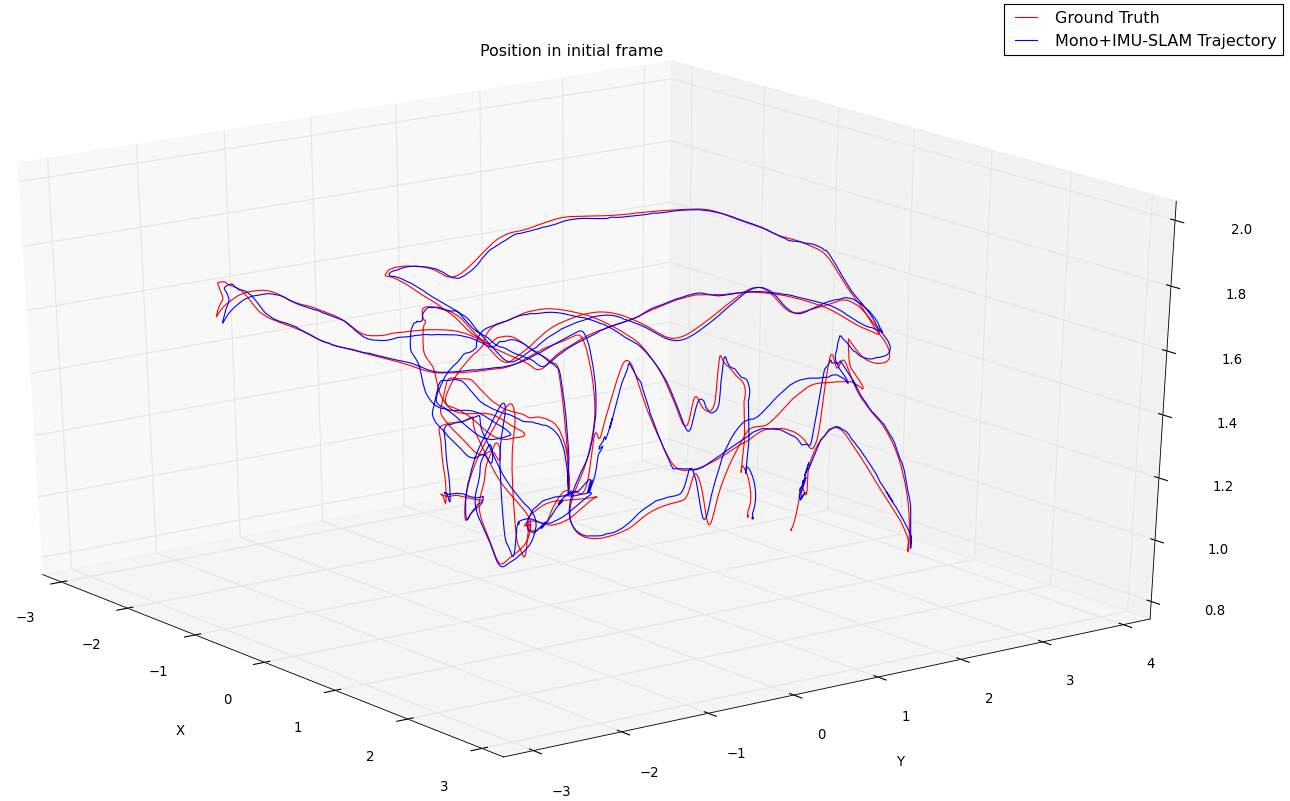
\includegraphics[scale=0.48]{figures/V1_01.png}  
	}
	\subfigure[V1\_ 02\_ medium]
    {	
		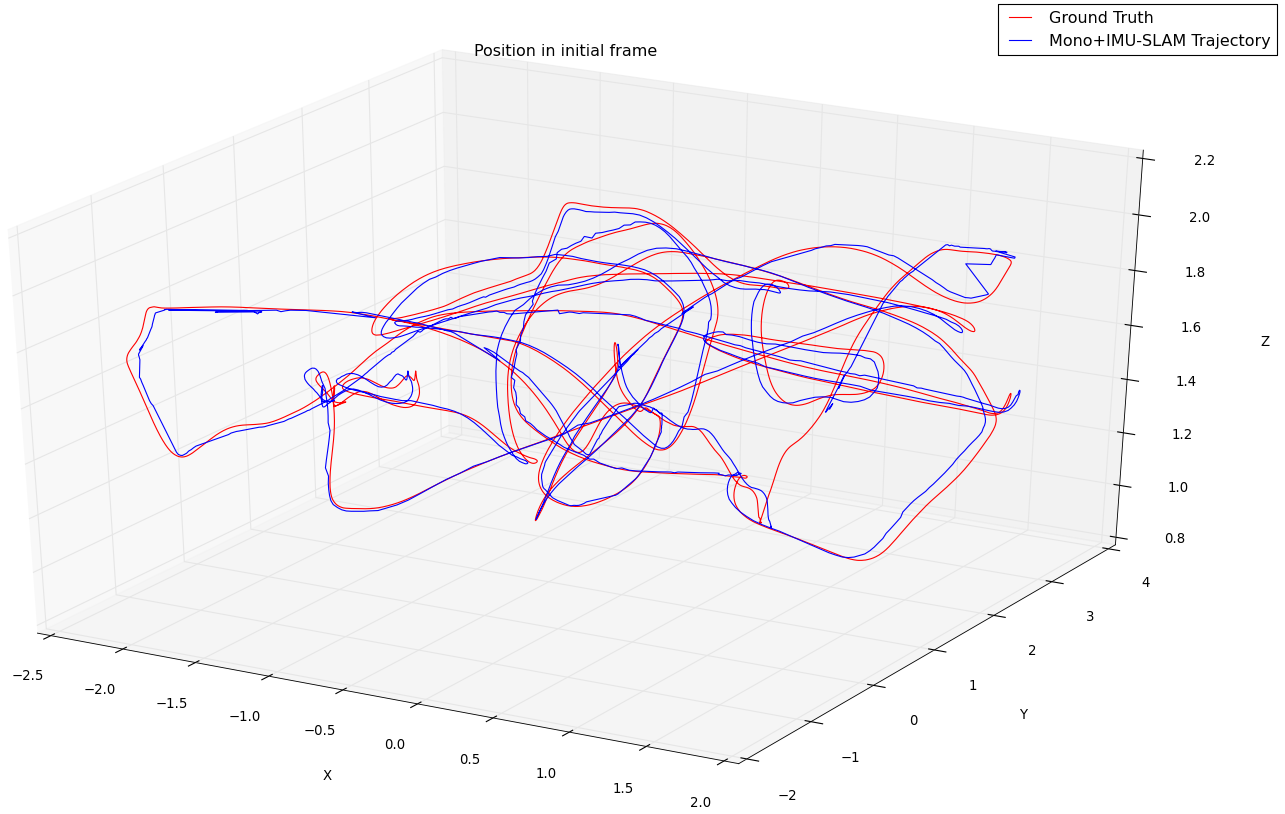
\includegraphics[scale=0.48]{figures/V1_02.png}
	}
\caption{V1飞行轨迹}
\end{figure}


\begin{figure}[h]
\centering
	\subfigure[MH\_ 02\_ easy]
    {
		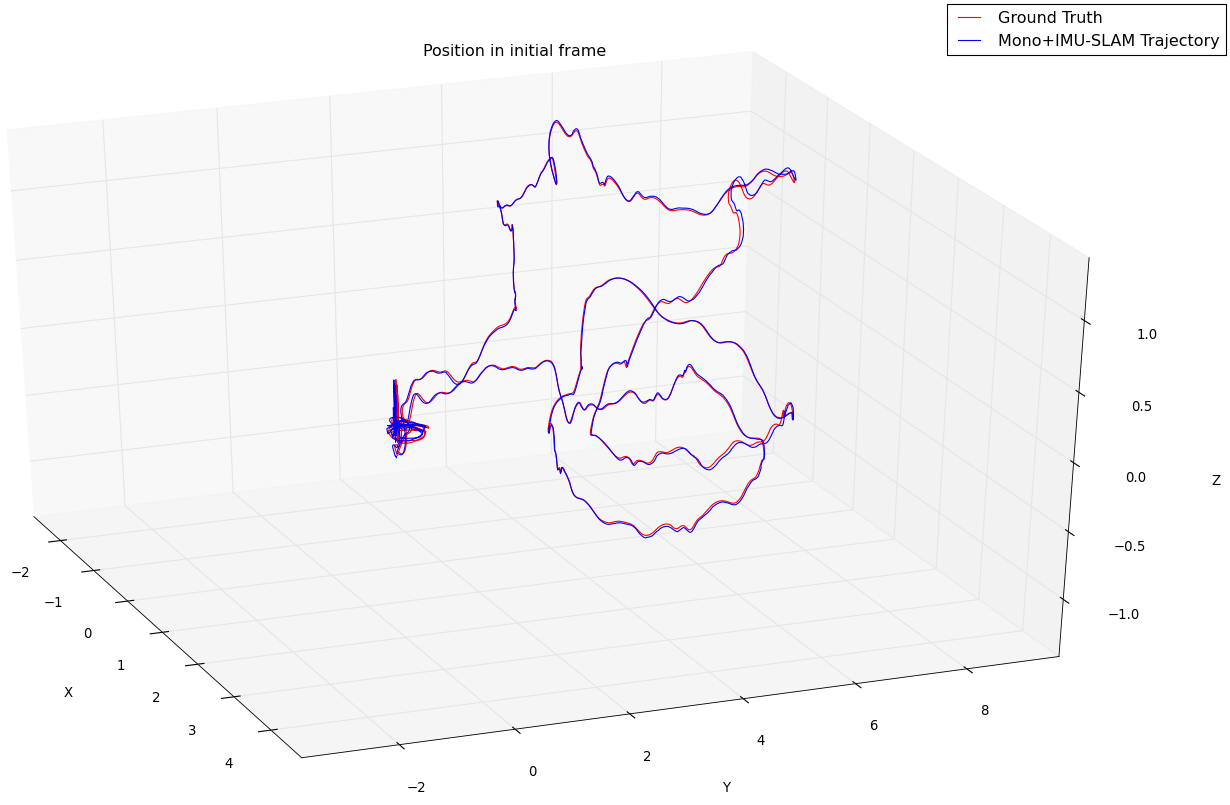
\includegraphics[scale=0.42]{figures/MH2.png}  
	}
	\subfigure[MH\_ 03\_ medium]
    {	
		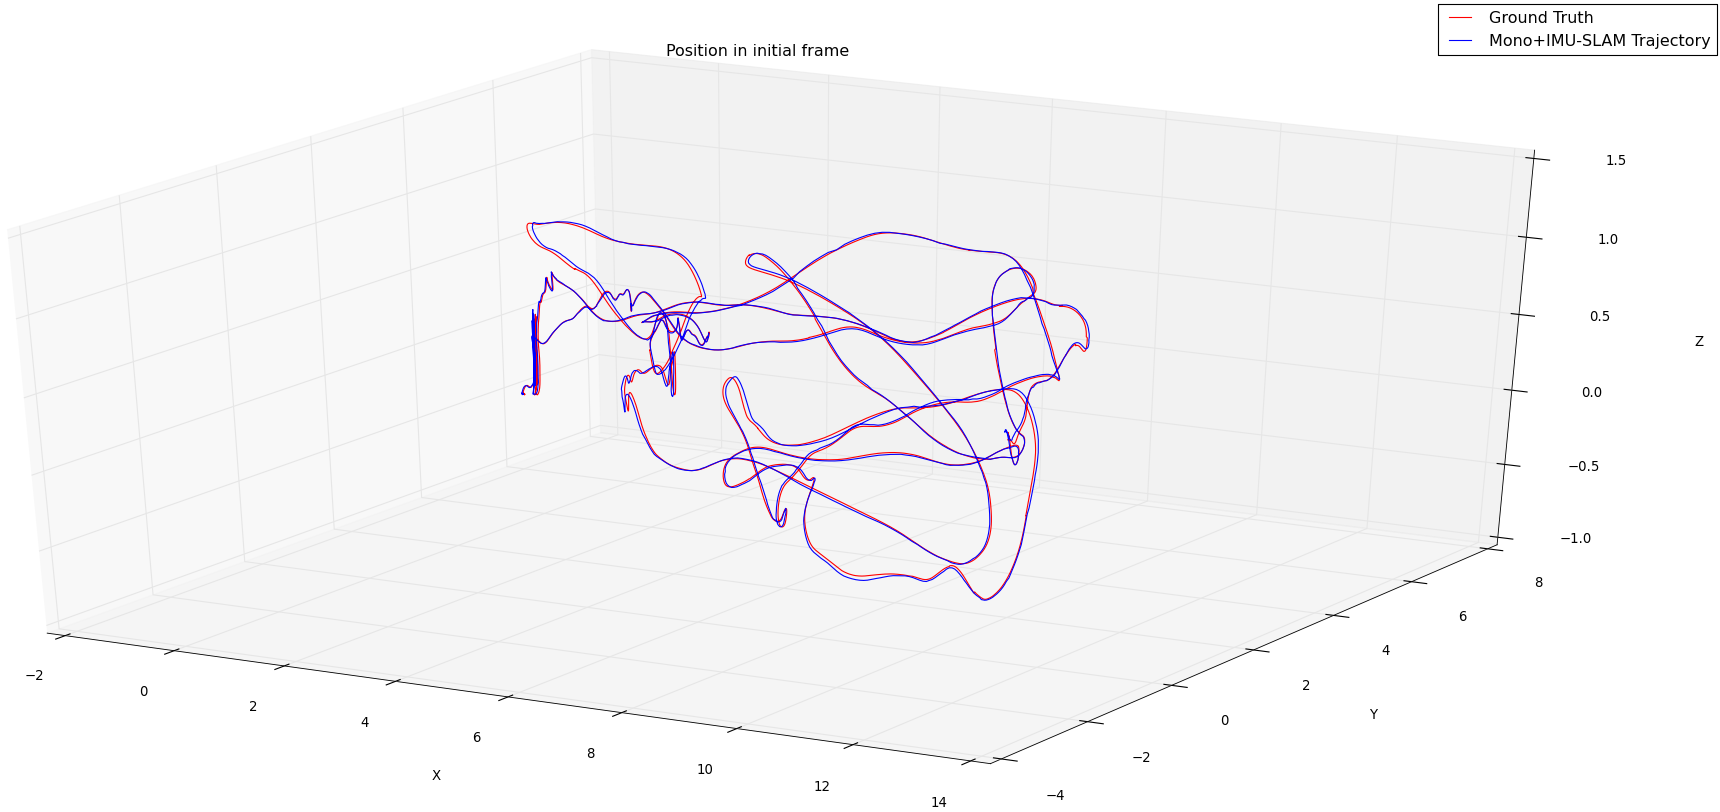
\includegraphics[scale=0.42]{figures/MH3.png}
	}
	\subfigure[MH\_ 04 \_ difficult]
    {	
		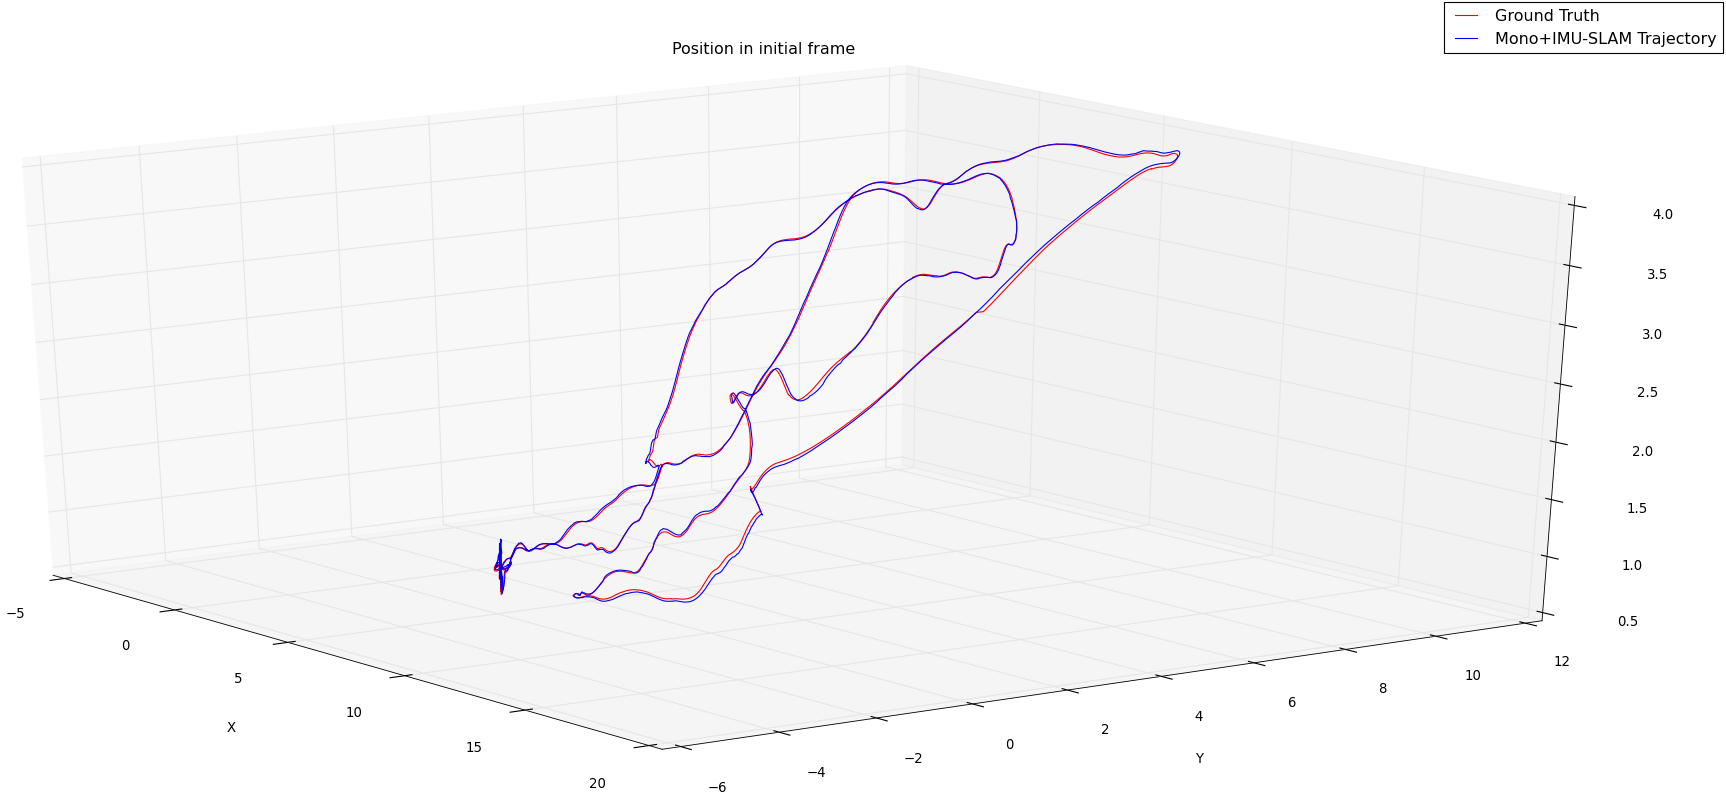
\includegraphics[scale=0.37]{figures/MH4.png}  
	}
\caption{MH飞行轨迹}
\end{figure}





 

%(其后部分无编号)
\backmatter

% 发表文章目录
%%==================================================
%% pub.tex for BIT Master Thesis
%% modified by yang yating
%% version: 0.1
%% last update: Dec 25th, 2016

%% modified by Meng Chao
%% version: 0.2
%% last update: May 29th, 2017
%%==================================================

\begin{publications}{99}

    \item\textsc{Chao Meng,Baiwei Guo,Xin Liu}. {Simultaneous localization and mapping using monocular direct method}[C]. Control, Automation, Robotics and Vision (ICARCV), 2016 14th International Conference on, IEEE, 2016: 1-5.(EI检索)
      
       \item\textsc{Xin Liu,Baiwei Guo,Chao Meng}. {A Method of Simultaneous Location and Mapping Based on RGBD Cameras}[C]. Control, Automation, Robotics and Vision (ICARCV), 2016 14th International Conference on, IEEE, 2016: 1-5.(EI检索)
    
\end{publications}
% 致谢
%%==================================================
%% thanks.tex for BIT Master Thesis
%% modified by yang yating
%% version: 0.1
%% last update: Dec 25th, 2016

%% modified by Meng Chao
%% version: 0.2
%% last update: May 29th, 2017
%%==================================================

\begin{thanks}

感谢我的导师郭百巍老师!本论文的工作是在导师郭百巍老师的指导下完成的。在北京理工大大学攻读硕士学位期间,无论在学习、科研方面还是生活上郭老师都给予了我很大的的指导和帮助,给了我很多十分有价值的想法和建议。郭老师科学严谨的治学态度、踏实勤奋的工作作风、渊博的知识,为我树立了学习的榜样,使我获益匪浅。在此,我向郭百巍老师表达由衷的感谢和敬意。

感谢实验室的师兄师姐师弟师妹们,正是实验室的浓厚的科研氛围熏陶了我,实验室的生活让我感受到集体大家庭的温暖。另外感谢宿舍的舍友在生活上的关心与照顾。在此,特别感谢徐勇老师、赵良玉老师、宋晓东老师、单家元老师、孟秀云老师、丁艳老师、王彦恺老师、张卫忠老师。在攻读硕士学位期间,课题组的老师们为我在科研工作上提供了思路,给予了我很大的帮助。

感谢我的父母家人以及女朋友,感谢你们无微不至的关怀与鼓励。正是你们在背后默默的支持和奉献才能使我顺利完成学业。

\end{thanks}

% 作者简介(博士论文需要)
%\include{chapters/resume}


\end{document}
